\documentclass[a4paper,12pt]{report}
\usepackage[hidelinks]{hyperref}
\usepackage{graphicx}
\usepackage{float}
\usepackage{caption}
\usepackage{array}
\usepackage{tabu}
\usepackage[tt]{titlepic}
\renewcommand\thesection{\arabic{section}}

%% ------------------------- Title Page ----------------------------
\titlepic{ \centering
\includegraphics[width=0.7\textwidth]{../images/dddd.png}  }

%\documentclass[12pt]{article}
\title{ \rule{\textwidth}{1pt}  \\ \Huge User Manual \\ 
	\Large Cafeteria Management System: Resolve Solution Partners (Pty) Limited \\
	\small Client: Gareth Botha and Jaco Pieterse}

\author{ 
         \underline{T-RISE}\\
          Rendani Dau (13381467) \\
	Elana Kuun (12029522) \\
	Semaka Malapane (13081129) \\
	Antonia Michael (13014171) \\
	Isabel Nel (13070305) \\ \\
	https://github.com/toniamichael94/MainProjectCOS301 \\ }
 

 
\date{\today \\ \rule{\textwidth}{1pt}}


\begin{document}
\maketitle
\break

%%------------------- Make table of contents-------------------
\tableofcontents
\break

%%-----------------------------Version table-------------------
\begin{figure}[H]
  \centering
   
\includegraphics[width=0.3\textwidth]{../images/cmslogo.jpg} 
\end{figure}
 \begin{tabu} to 0.8\textwidth { | X[l] | X[l] | }
 \hline
 \textbf{Document Title} & User Manual \\
 \hline
 \textbf{Document Identification}  & Document 0.0.8  \\
 \hline
 \textbf{Author}  & Rendani Dau, Isabel Nel, Elana Kuun, Semaka Malapane, Antonia Michael \\
 \hline
 \textbf{Version} & 0.0.8 \\
 \hline
 \textbf{Document Status} & Eighth Version - edited entire document with changes and added new pages for reporting and graphs\\
 \hline
 \end{tabu}

\begin{table}[h!]
\centering
 \begin{tabular}{||c c c c||} 
 \hline
 \textbf{Version} & \textbf{Date} & \textbf{Summary} & \textbf{Authors} \\ [0.5ex] 
 \hline\hline
 0.0.1 & 9 July 2015 &  First draft contains how to run system  & Rendani Dau, \\ & & & Elana Kuun, \\ & & & Semaka Malapane, \\ & & & Antonia Michael \\ & & & Isabel Nel, \\ & & & \\
 \hline 
 & & & \\
 0.0.2 & 20 July 2015 &  Second draft adding page  & Rendani Dau, \\ & & assistance and explanation & Elana Kuun, \\ & & of how to use & Semaka Malapane, \\ & & functionality on page &  Antonia Michael \\ & & & Isabel Nel \\   [1ex]  
 \hline 
 & & & \\
 0.0.3& 23 July 2015 &  Third draft containing  & Rendani Dau, \\ & & screenshots of the & Elana Kuun, \\ & & of different page & Semaka Malapane, \\ & & and their functionality &  Antonia Michael \\ & & & Isabel Nel \\   [1ex]  
 \hline
 & & & \\
 0.0.4& 3 August 2015 &  Fourth draft Added  & Rendani Dau, \\ & & Troubleshooting & Elana Kuun, \\ & & Section & Semaka Malapane, \\ & &  &  Antonia Michael \\ & & & Isabel Nel \\   [1ex]  
  \hline 
 & & & \\
 0.0.5& 28 August 2015 &  Fifth draft containing  & Rendani Dau, \\ & & screenshots of the & Elana Kuun, \\ & & of different page & Semaka Malapane, \\ & & and their functionality &  Antonia Michael \\ & & & Isabel Nel \\   [1ex]  
  \hline 
 & & & \\
 0.0.6& 22 September &  Sixth draft containing  & Rendani Dau, \\ & & edited according to & Elana Kuun, \\ & & feedback given & Semaka Malapane, \\ & & and add new content &  Antonia Michael \\ & & & Isabel Nel \\   [1ex]  
 \hline 
 & & & \\
 0.0.7& 9 October &  Seventh draft containing  & Rendani Dau, \\ & & added audit, notifications, & Elana Kuun, \\ & & statistics, & Semaka Malapane, \\ & &  and themes &  Antonia Michael \\ & & & Isabel Nel \\   [1ex]  
 \hline 
 & & & \\
 0.0.8& 16 October &  Eighth draft containing  & Rendani Dau, \\ & & edits and additions to & Elana Kuun, \\ & & the document, & Semaka Malapane, \\ & &  document &  Antonia Michael \\ & & & Isabel Nel \\   [1ex]  
\hline
 \end{tabular}
\end{table}

\pagebreak
\pagebreak
%%now begin document
%%---------------------------------  INTRODUCTION -------------------------------------------

\section{Introduction} 
This document contains the user manual for the Resolve Cafeteria Management System that will be created for Software Engineering (COS 301) at the University of Pretoria 2015, by the group T-RISE.

%% ------------------------------ VISION ------------------------------------------------------
\section{Vision}
The vision of this project is to implement a fully functional software application that will be maintainable, with detailed supporting documentation and an instruction manual for the Cafeteria Management System. This system will, amongst others, assist in executing orders from the cafeteria, managing the cafeteria's inventory, generating bills, and perform various reporting tasks. 

%%---------------------------------- INTRO -----------------------------------------
\section{Background}
\subsection{The current situation/ problems the client currently experience}
As specified in the project proposal document from Resolve, the cafeteria is currently cash only and does not accept bank cards or electronic payments. This is inconvenient for employees as they have to carry around cash if they want to purchase anything from the cafeteria. Employees may choose to go to an external food outlet where they can pay with their preferred method of payment, which uses time and fuel. Thus, this means the cafeteria does not achieve the maximum amount of income which hinders its growth and improvement.\\ A problem with the cafeteria itself is that certain meal items are hardly in stock due to either lack of ingredients to make the meal or under estimating the quantity of the meal item required.

\subsection{How the aforementioned problems will be alleviated by the CMS}
The Cafeteria Management System will provide a means to accept payments from employees, at the canteen, using their employee access cards or access card numbers, with an amount being deducted from their salary at the end of the month.  The option of cash payments ,however, will not be discarded. At the end of each month, the bill for the month will be sent to either payroll, to the employee, or to both. This option is thus configurable from the user's profile. The employee can also set a spending limit for each month. There will also be a system wide limit that users cannot exceed.
\\
The system will predict which inventory items needs to be bought for the next week in order to avoid the "out of stock" situation described above. The system will also enforce that when the cafeteria manager adds meal items to the menu, he adds inventory items for each menu item. This is done so that each time a menu item requires an inventory item, the quantity of the inventory item will decrement until it reaches zero and is marked as "Out of Stock" on the menu. This is done so that when the user is ordering food, he/she can clearly see which items are not in stock and hence does not need to find this out at the canteen.
\\
%%---------------------------------- SYSTEM OVERVIEW -----------------------------------------
\section{System Overview}
The Cafeteria Management System is a system designed to assist users to order food efficiently from their office's canteen and to be notified when their order is ready for collection. The system will also assist cafeteria staff with keeping track of the orders in real time as well as managing inventory. The system will also provide for configuring the branding settings of the cafeteria. The system is intended to be used in a corporate environment whereby users have the option to allow their cafeteria expenses to be deducted from their salary or immediately pay for orders. In addition, the system will allow management to view the bill reports of the different users. All users will also be able to access their spending history, set favourites and other similar functionality which will all be explained in this user manual. \\

%%--------------------------------------SYSTEM CONFIGURATION ----------------------------------------
\section{System Configuration}
The system requires a Windows/Unix based host to run the server. This host must have the associated technologies installed (the installation of these technologies will be discussed below). The host must be connected to the internet in order to allow any required dependencies to be installed and set up for the operating system environment. The configuration of the server requires an active email account to facilitate communication between the system and end users. 
End users will only require a PC equipped with a web browser such as Mozilla, Chrome or Internet Explorer, as well as an active internet connection.  
The types of data that will communicated and stored will be data of the NoSQL database MongoDB. The menu items that the cafeteria manager will add to the menu will be stored in the database, to be communicated/displayed on the menu page. The inventory items that these menu items entail will be stored too. The categories that can be added to the menu by the cafeteria manager will also be stored in the database in order to populate the navigation bar, the actual dynamic pages and various other places in which these are displayed. The cafeteria manager is the only user who is able to retrieve the menu and inventory data, in order to edit or delete it. The other users will just be able to view the menu data on the menu page. 
\\
The user's sign up information will also be stored and will be communicated on the profile page of the user. Each user will only have access to their own information. The superuser, however, will be able to search for users and update their IDs or delete them from the system.
\\

 The branding information such as the cover carousel images, the theme, the contact information and the canteen name will also be stored to be communicated on various pages. The superuser is the only user who be able to edit and add this information. Other settings that the superuser can configure, are the system limit and the roles of the users will be stored and used for determining the privileges associated with the various roles and the checks done on the users' personal spending limits. The superuser will also have access to the audit trail of all actions performed on the system. The finance manager will have access to the order history of each user in order to view their bills and invoices. The cashier will also have access to the orders placed in order to process them i.e. mark an order as ready and as completed. All the crucial information such as the order history and other changes made will be stored in an auditing table. Each user will have access to their personal spending history as well as a notifications page, populated with "Order pending" and "Order ready" notifications.
\begin{figure}[H]
  \centering
    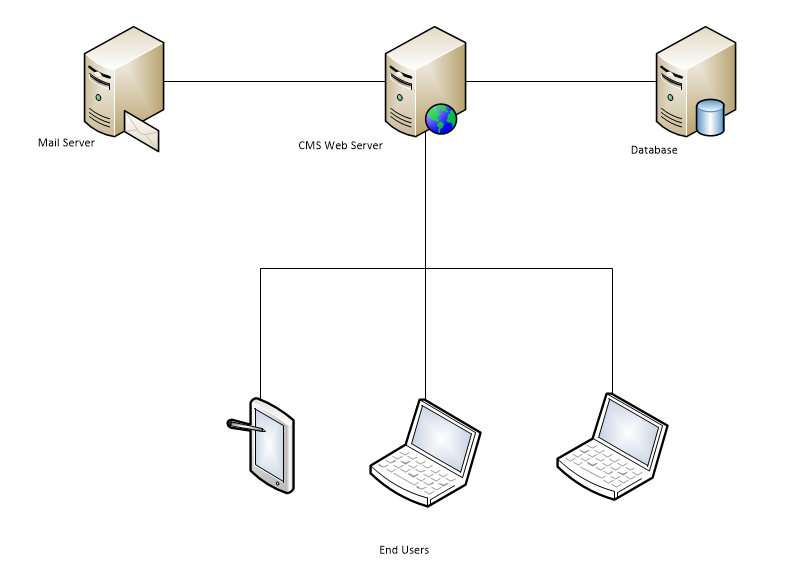
\includegraphics[width=1.0\textwidth]{screenshots/ServerClients.png}
    \caption{Overview of System - Servers and Clients} 
\end{figure}

%%--------------------------------------INSTALLATION  ----------------------------------------
\section{Installation}

%%------------------------PREREQUISITES ----------------------------
\subsection{Prerequisites}
For the programmer, who will maintain the code: \\ 
\\The  Cafeteria Management System must have the associated technologies, NodeJS, MongoDB, AngularJs, Express, Bower and grunt installed on the host (the installation of these technologies will be discussed below). These are free and open source software and can be obtained from the following sites:\\
\url{https://nodejs.org/download/} \\
\url{https://www.mongodb.org/downloads} \\
The applications are available for both Windows and Unix environments and include setup guides on their respective web pages.\\

Once installed, NodeJS includes a package manager called NPM. This package manager will be available from the terminal and will be used to install all dependencies. The following dependencies have to be installed first (Run these commands one by one in the command prompt or terminal):
\begin{verbatim}
$npm install -g bower
$npm install -g grunt-cli
\end{verbatim}

After these commands have successfully installed the respective applications you can download the Cafeteria Management Software from the GitHub repository :
 \url{https://github.com/toniamichael94/MainProjectCOS301}
\\ \\
This can be done by cloning the repository onto a remote location on your PC, if you do not know how to clone a GitHub repository, please visit:\\
  \url{https://git-scm.com/book/en/v2/Git-Basics-Getting-a-Git-Repository}  under the section "How to clone an existing repository" you will find the GitHub documentation on how to do this.
\\
Once you have cloned the GitHub repository and installed the above mentioned technologies, please move on to the next section , which will take you step by step in configuring the Cafeteria Management System (CMS).
\\ \\
{\em Please note that 'CMS' will be referred to in the rest of this document as an abbreviation for the Cafeteria Management System}


%%------------------------SETTING UP CMS ----------------------------
\subsection{Setting up CMS}
For the programmer, who will maintain the system: \\
Before starting the system, an email account has to be set up to facilitate communication between the system and end users. The details of this account can be configured in the following config file:
\begin{verbatim}
	~/Cafeteria_Management_System/config/env/production.js
\end{verbatim} 
{\em (The document can be opened in any text editor or IDE  such as NetBeans, WebStorm or atom - just to name a few )}
\\ \\
Under the section 'Mailer', the following fields should be specified:\\
\begin{itemize}
\item MAILER\textunderscore FROM: A name indicating the sender of mail.
\item MAILER\textunderscore SERVICE\textunderscore PROVIDER: The service provider of the email account
\item MAILER\textunderscore EMAIL\textunderscore ID: The email ID of the account set up for CMS
\item MAILER\textunderscore PASSWORD: The password of the account set up for CMS
\end{itemize}


In a terminal/command prompt, navigate to the CMS directory and execute the 'npm install' command. This will install all the packages required to run the system: 


\begin{verbatim}
~/  Cafeteria_Management_System/ $npm install
\end{verbatim}

If all dependencies were installed successfully, then MongoDB can be started with the following command in a completely new terminal or command prompt:
\begin{verbatim}
~/$mongod --dbpath "directory"
\end{verbatim}

Where "directory"  is a path to the folder which Mongo will use as a working directory.\\ \\
{\em Remember that this command has to be executed in a separate terminal.}\\ \\
Below is an example of what the output should look like :

\begin{figure}[H]
  \centering
    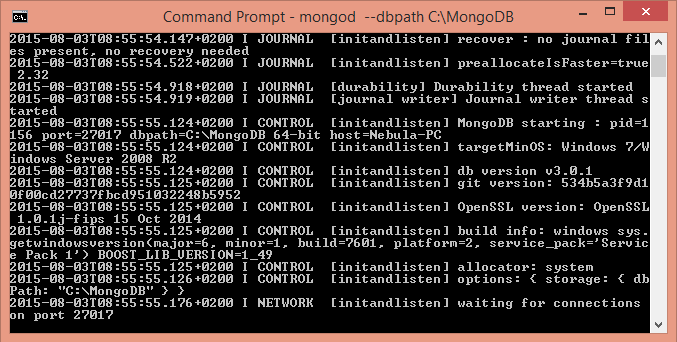
\includegraphics[width=1.0\textwidth]{screenshots/MongoDB.png}
    \caption{MongoDB Terminal - Expected output when running MongoDB} 
\end{figure}

Once mongo has been started, the CMS server can be started with the following command:\\ \\

\begin{verbatim}
~/Cafeteria_Management_System/$ grunt
\end{verbatim}

\begin{figure}[H]
  \centering
    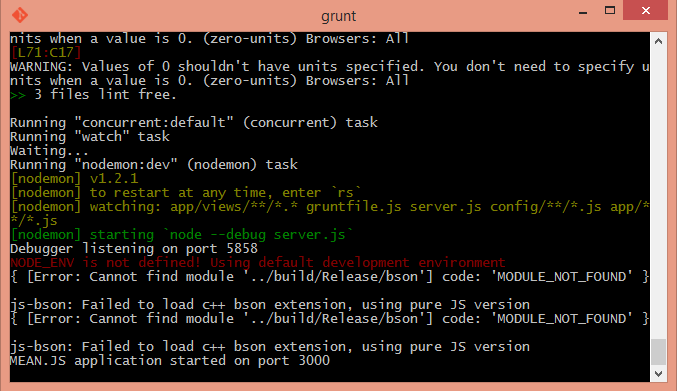
\includegraphics[width=1.0\textwidth]{screenshots/gruntOutput.png}
    \caption{Grunt - When grunt is running, output should be similar to this.} 
\end{figure}

Now the Server and the Database are running and we can get started with the rest of the setup process. \\
Note: Inside the browser one will run localhost:3000 to view system. \\ 

To terminate the server, the user can enter the Ctrl+C command in the "grunt" terminal. The user can also terminate the MongoDB service by executing the same command (Ctrl+C) in the MongoDB terminal.

%%-------------------------------------GETTING STARTED ----------------------------------------
\section{Getting Started}
Access to the Cafeteria Management System is through a standard web browser. Different types of users have access to different facets of the system. The system has a default super user account and an admin user account, where both of these users can assign different roles (cafeteria manager, cashier, etc.) to the users. They also have global access to the whole system. These users can then sign in to access the facet of the system they are authorised to.\\

%%--------------------------------ADMINISTRATIVE USERS -------------------------
\subsection{Administrative Users}
When the CMS is started initially with an empty database there will be no users in the database and this includes no administrative users.  \\
Thus, to generate the administrative users, on the first startup of the system, one should navigate to the sign in page and sign in with empty credentials. If the system is started for the first time with an empty database, on sign in with empty credentials (proceeding to submit the signin form without filling in username or password) administrative users will be created. \\

\textbf{The system will have a Super User:} \\
Employee ID: SuperUser \\
Password: SuperUser \\

\textbf{And the system will also have an Admin User:} \\
Employee ID: AdminUser \\
Password: AdminUser \\

\textbf{WARNING :} \\
Administrative users will have global access to the whole system, thus it is of utmost importance that the administrative users should be set up with the first start up of the system and their credentials should immediately be changed for security. \\ 

{\em* Note at all times there can only be 1 super user and 1 admin user - this is done for security purposes  } \\
 

%%-------------------------------- CREATING AN ACCOUNT -------------------------
\subsection{Creating an Account} 
Once the user has clicked the "Sign Up" option on the navigation pane, the user will be directed to the signup form, where the user should fill in their details. 

\begin{figure}[H]
  \centering
    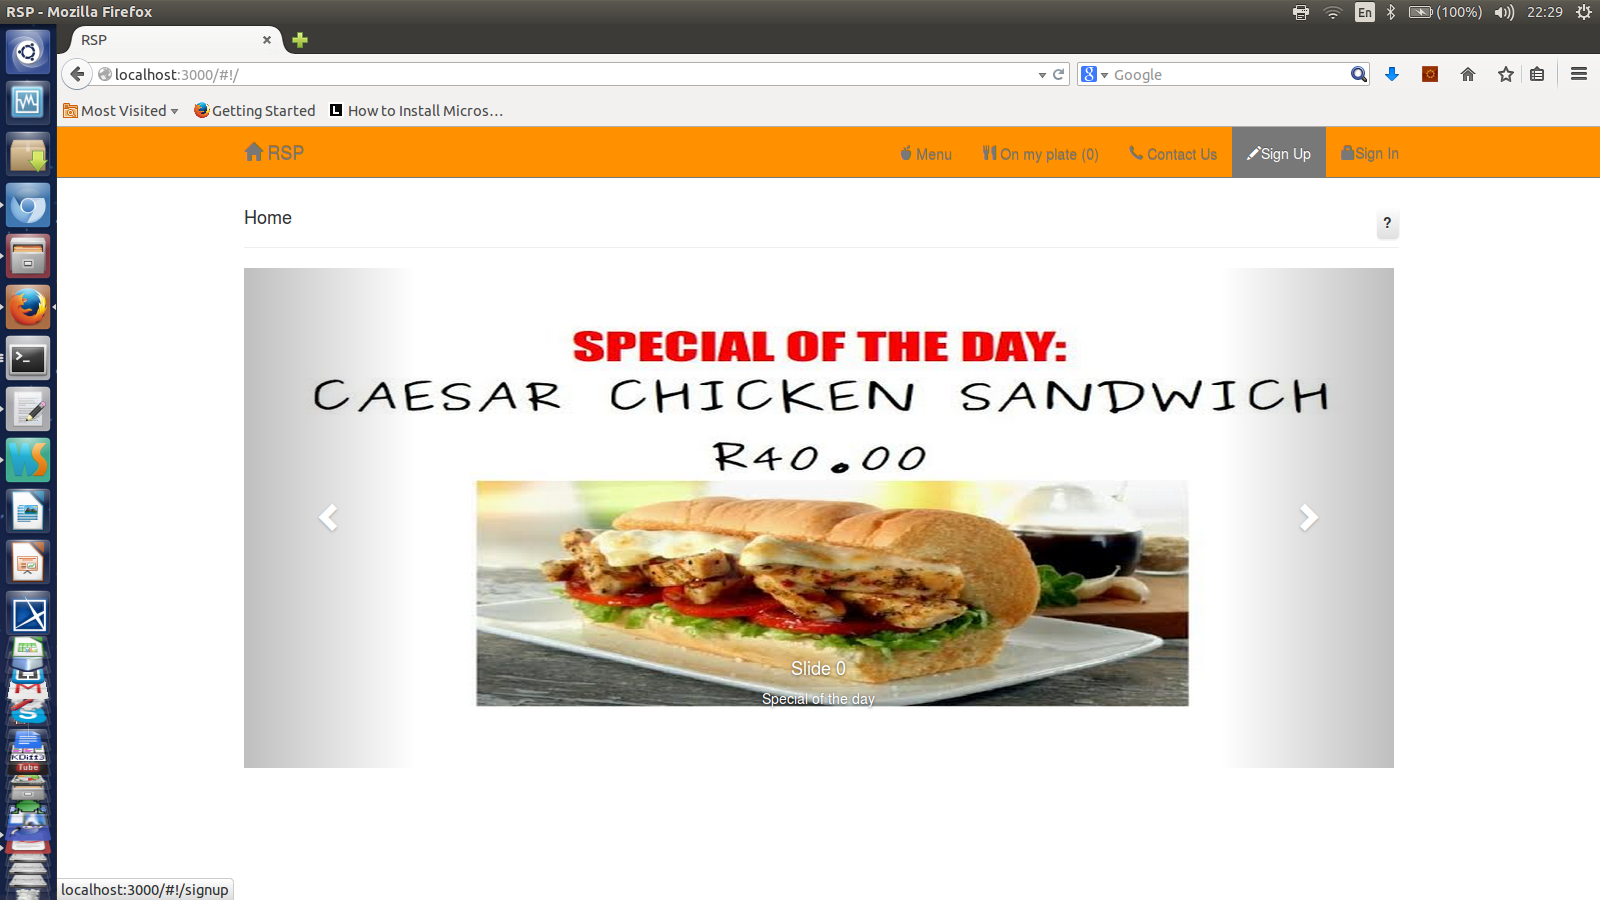
\includegraphics[width=1.0\textwidth]{screenshots/signUp.png}
    \caption{Sign Up - as indicated by the grey box on the page} 
\end{figure}

When the button is clicked, the CMS will direct the user to the signup page where the user can fill out all the details. Once the user have completed the form, the user will click submit and if the form is correctly filled in , the user will be notified upon success and will be signed up for the system. They will hence be redirected to the home page. The user will then use the password created and employee ID to log in to the system. If the information entered is not valid, a thorough error message will be displayed indicating what the problem is so that the user can rectify it.

\begin{figure}[H]
  \centering
    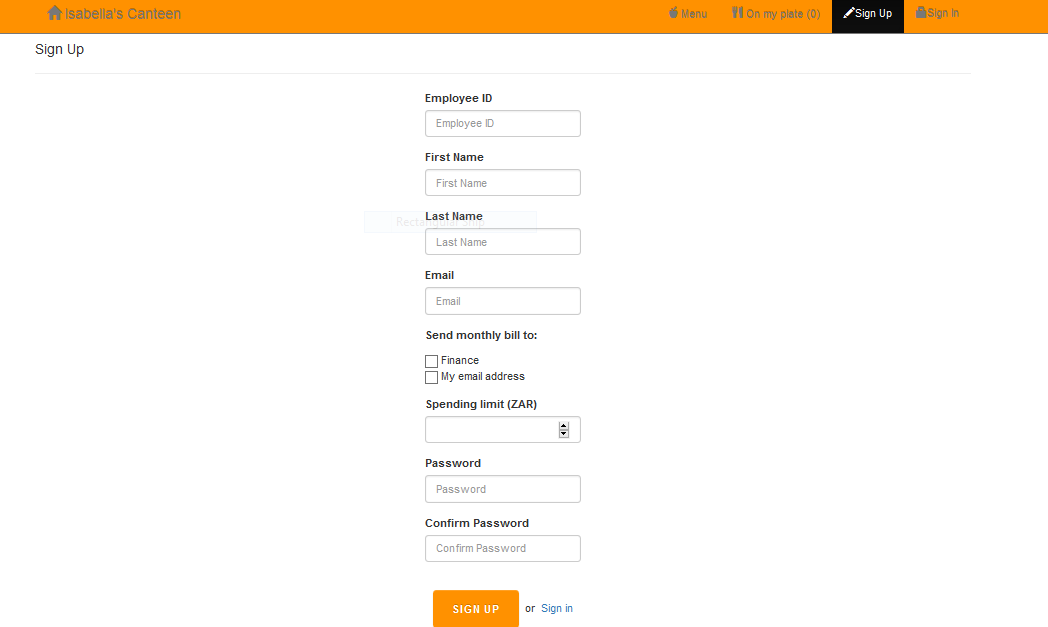
\includegraphics[width=1.0\textwidth]{screenshots/signUpPage.PNG}
    \caption{Sign Up Page - details to be filled in - all fields are required} 
\end{figure}

{\em Employee ID } will be assigned to users by their company - no Employee ID can be reused.\\
The {\em e-mail address} to receive notifications of when their orders are ready and to receive monthly financial bills. \\
The {\em spending} Limit is the maximum amount you may spend each month.\\

{\em Note that all the fields may be edited when logged in} \\

After signing up and creating a new account the user will automatically be logged in. 

%%-------------------------------- LOGGING IN  -------------------------
\subsection{Logging In}
To sign in, the user must click on the 'Sign In' tab on the navigation bar.

\begin{figure}[H]
  \centering
    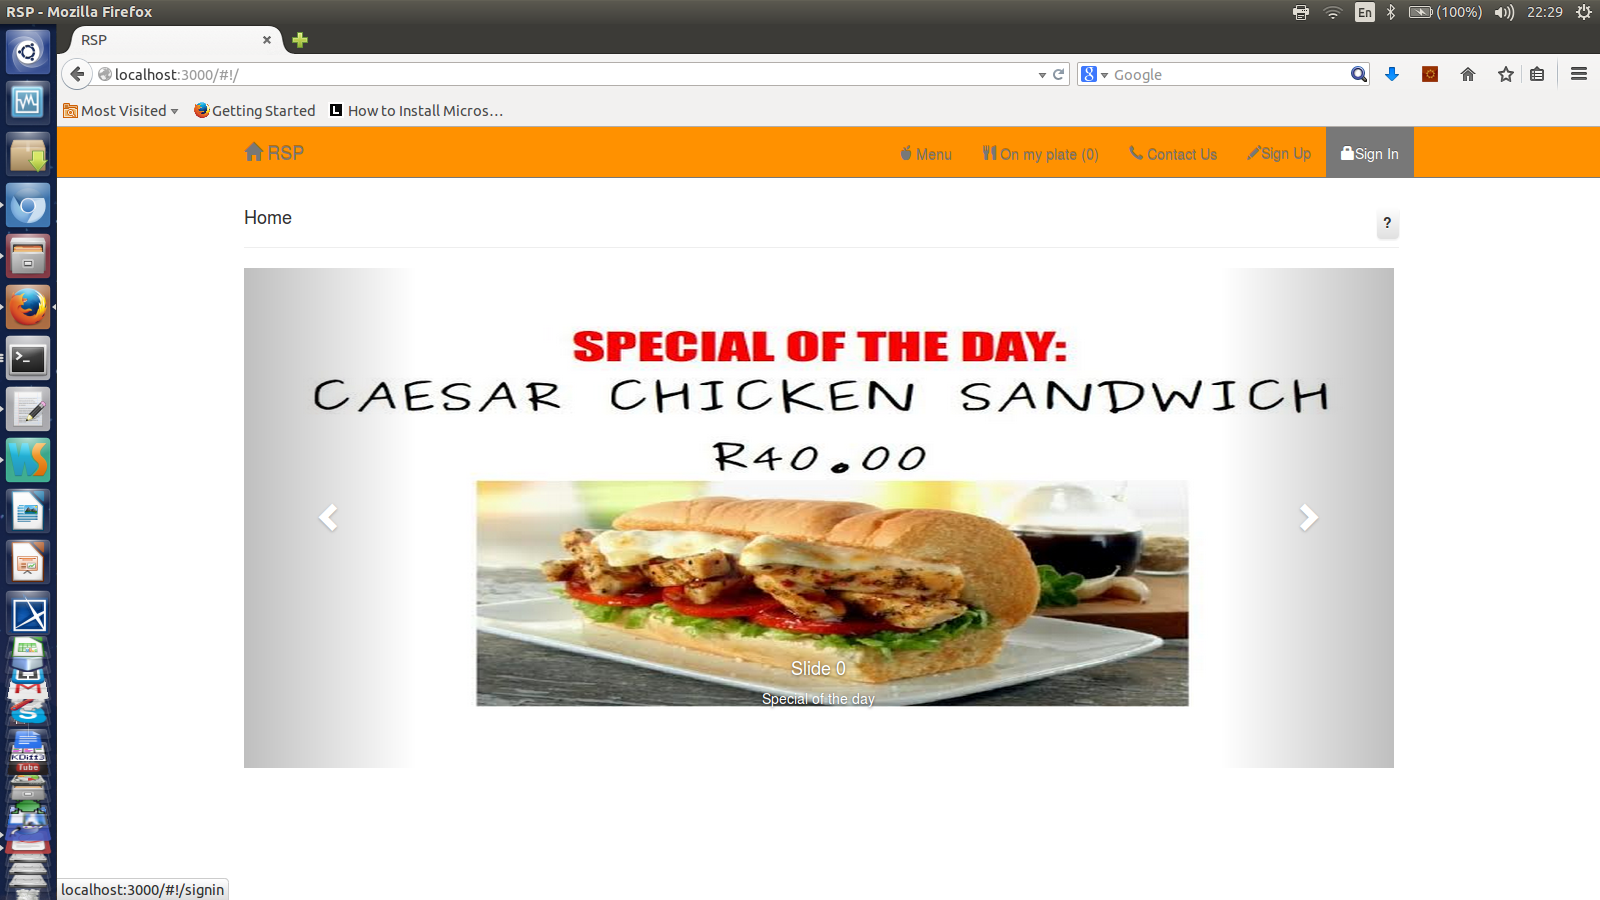
\includegraphics[width=1.0\textwidth]{screenshots/signIn.png}
    \caption{Sign In - as indicated by the grey box on the page} 
\end{figure}

Once the user clicks on the sign in tab, the CMS should direct to the sign in page :

\begin{figure}[H]
  \centering
    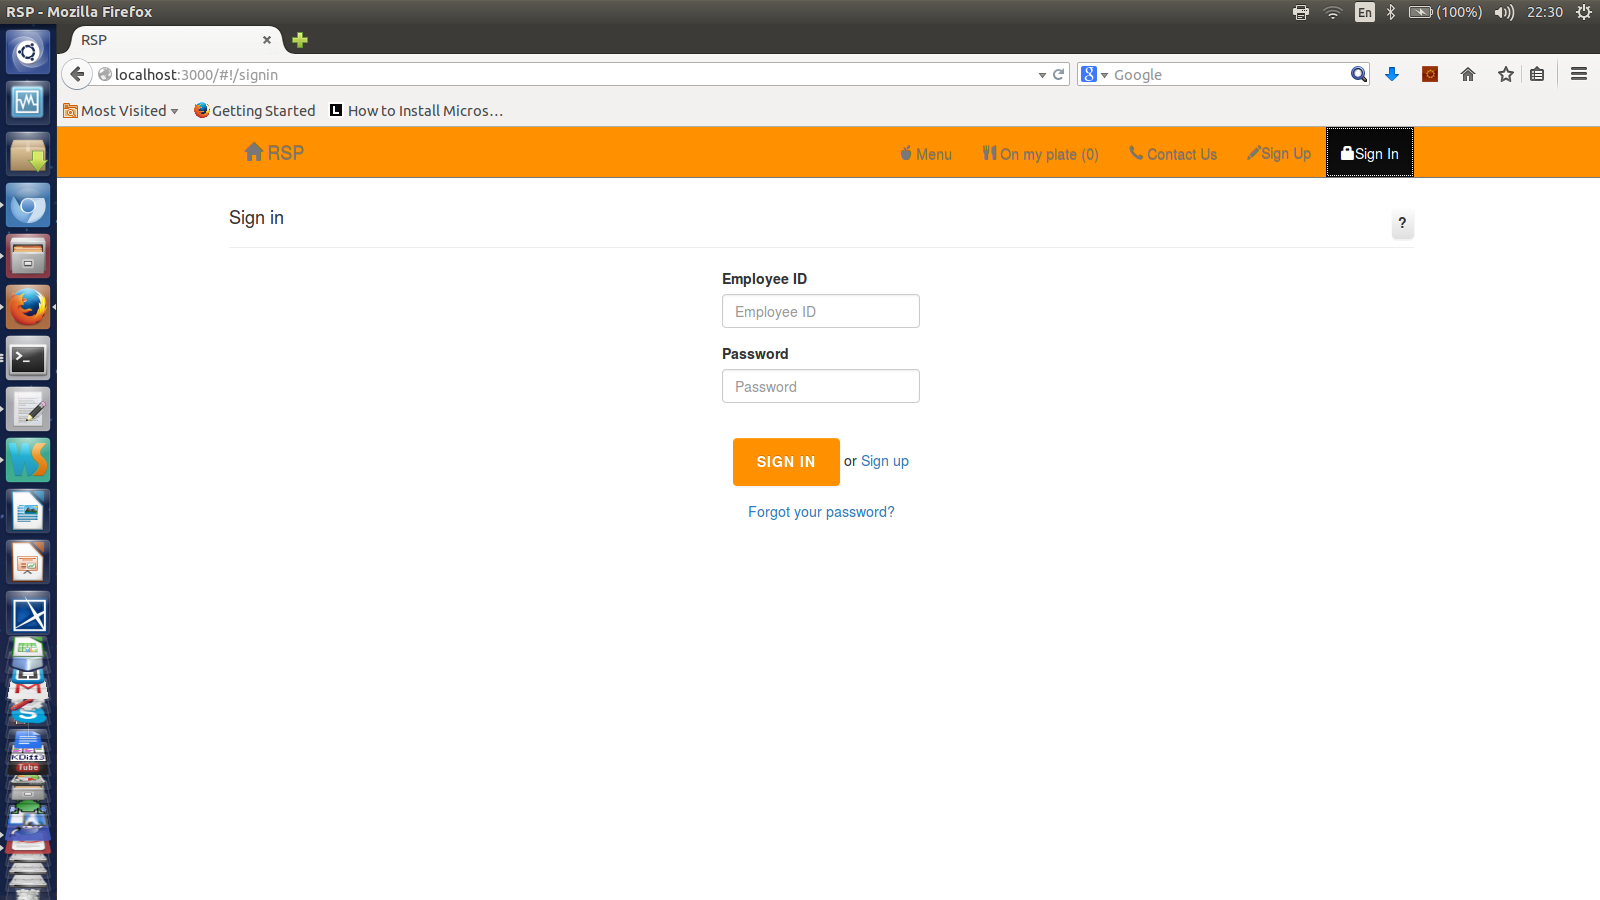
\includegraphics[width=1.0\textwidth]{screenshots/signInPage.png}
    \caption{Sign In page - Type the appropriate information in the textboxes and click submit to sign in} 
\end{figure}
  
The user will fill in their password and Employee ID in the provided slots and click submit to proceed. If the information entered is valid, the user will be notified upon success and redirected to the home page, logged in on their personal account. If the information entered is not valid, a thorough error message will be displayed indicating what the problem is so that the user can rectify it.
If the user can not login due to forgetting his/her password they can click on the forget password link which will redirect to the forget password page:
 
\begin{figure}[H]
  \centering
    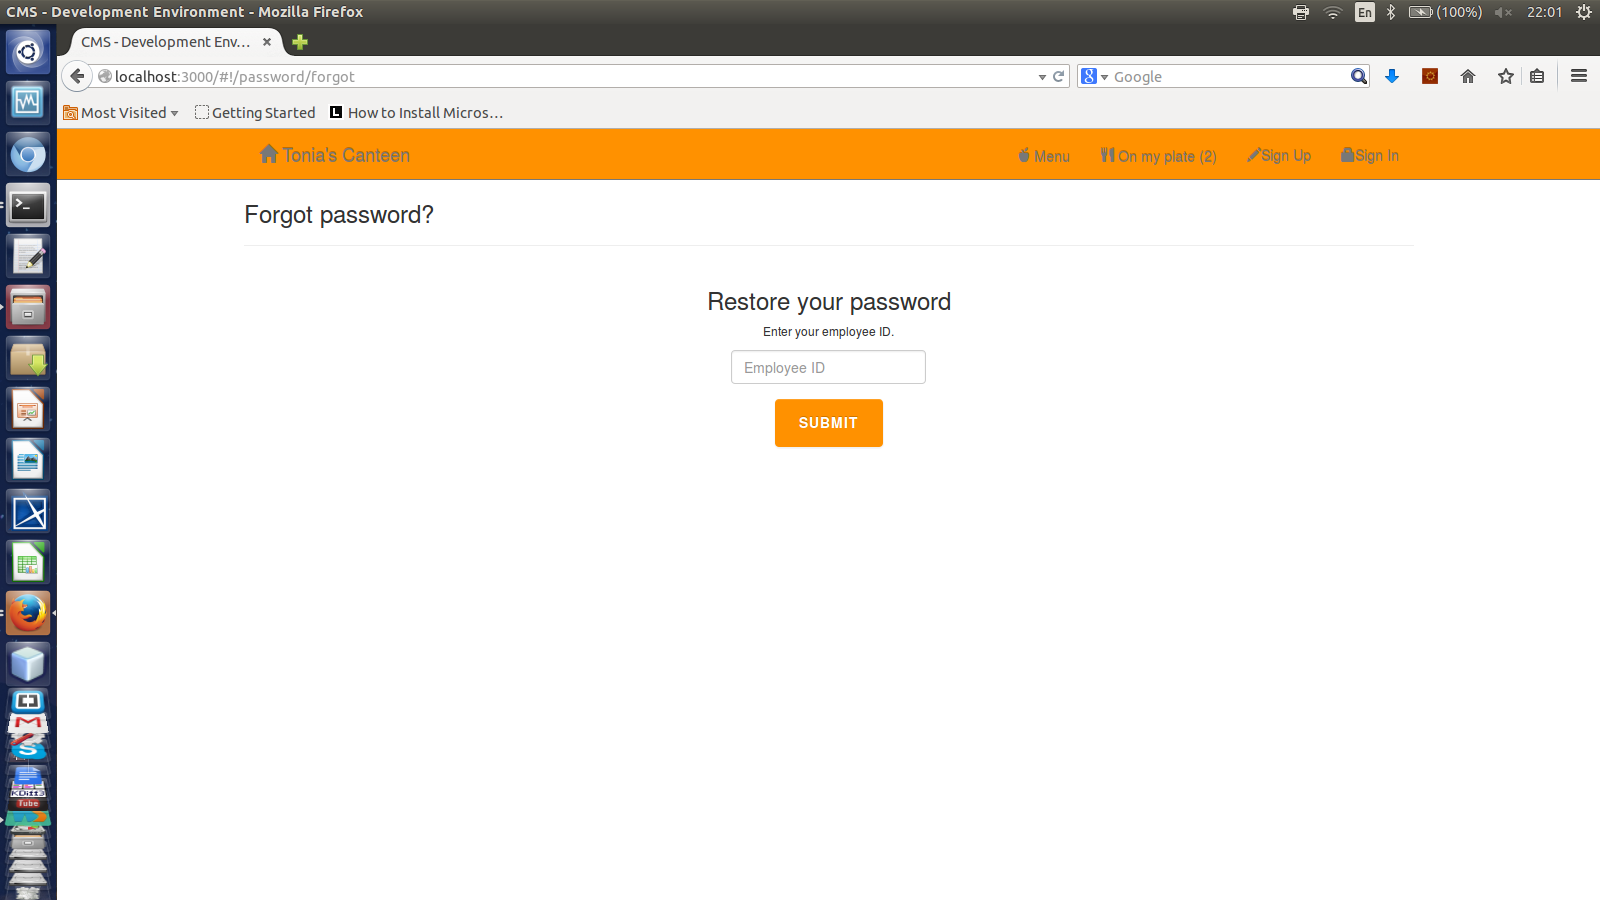
\includegraphics[width=1.0\textwidth]{screenshots/ForgotPass.png}
    \caption{Forgot password page} 
\end{figure}

The "Forgot your password?"option, which once clicks leads the user to a page where the user must enter their Employee ID. The user will then be notified that an email has been sent to their personal email account with further instructions on how to rectify the situation. The user will be sent a link to a page, in order to set a new password.    \\

The rest of the functionality will be described in the section below in detail  under the respective headings of how to navigate between pages to administrative settings to ordering an item and so forth. 
 
\begin{figure}[H]
  \centering
    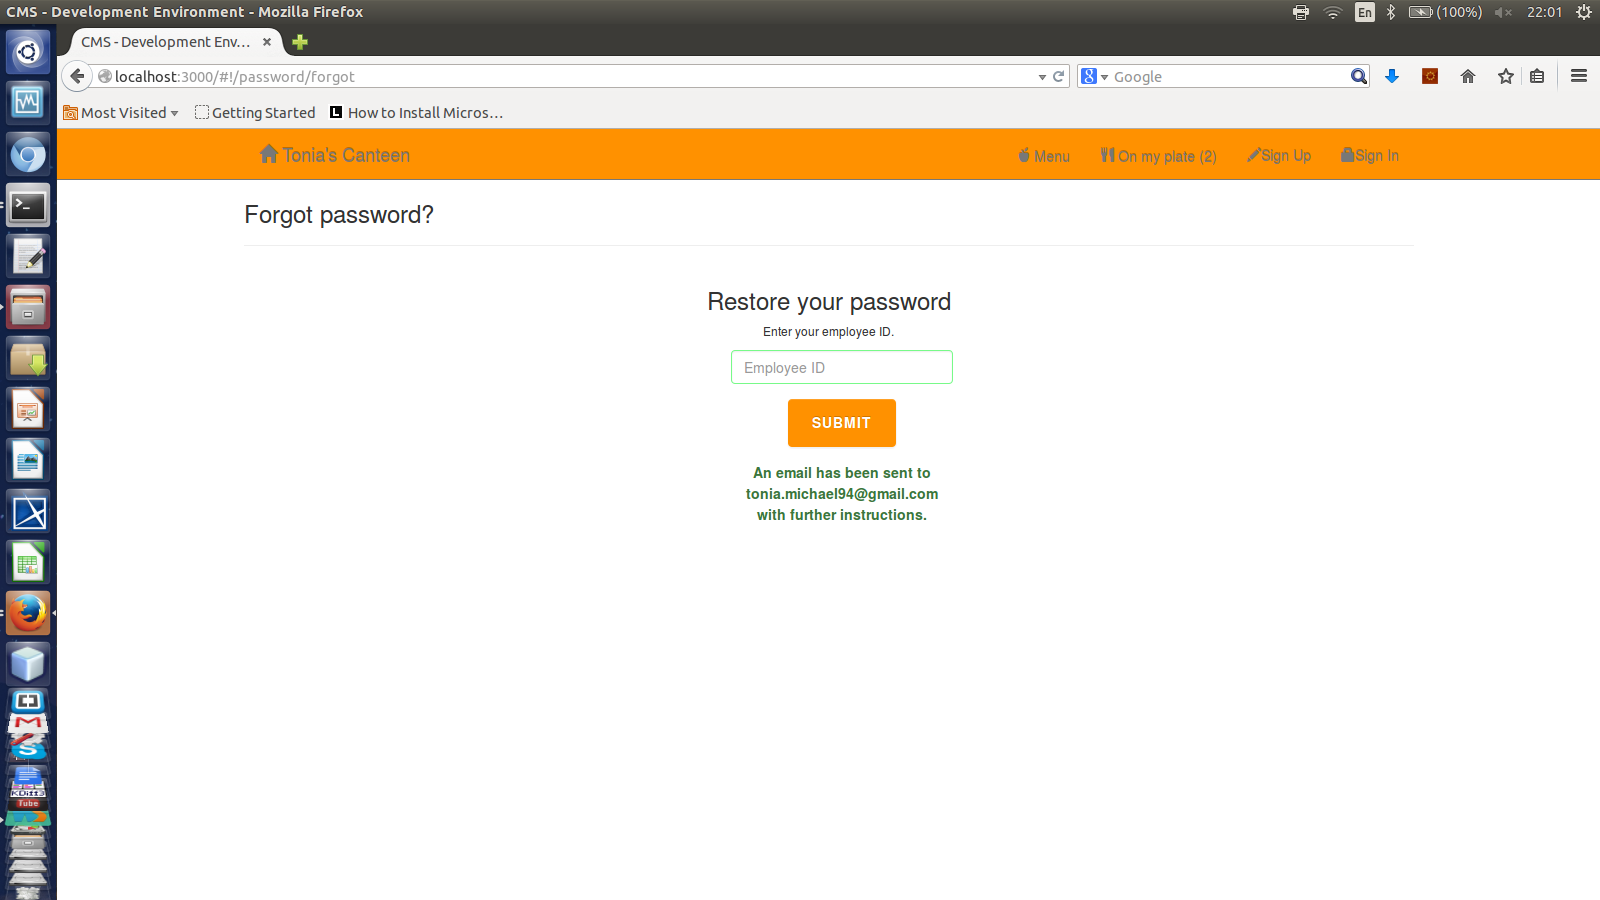
\includegraphics[width=1.0\textwidth]{screenshots/emailSentForPass.png}
    \caption{After submitting the form - notified about email sent} 
\end{figure}

\begin{figure}[H]
  \centering
    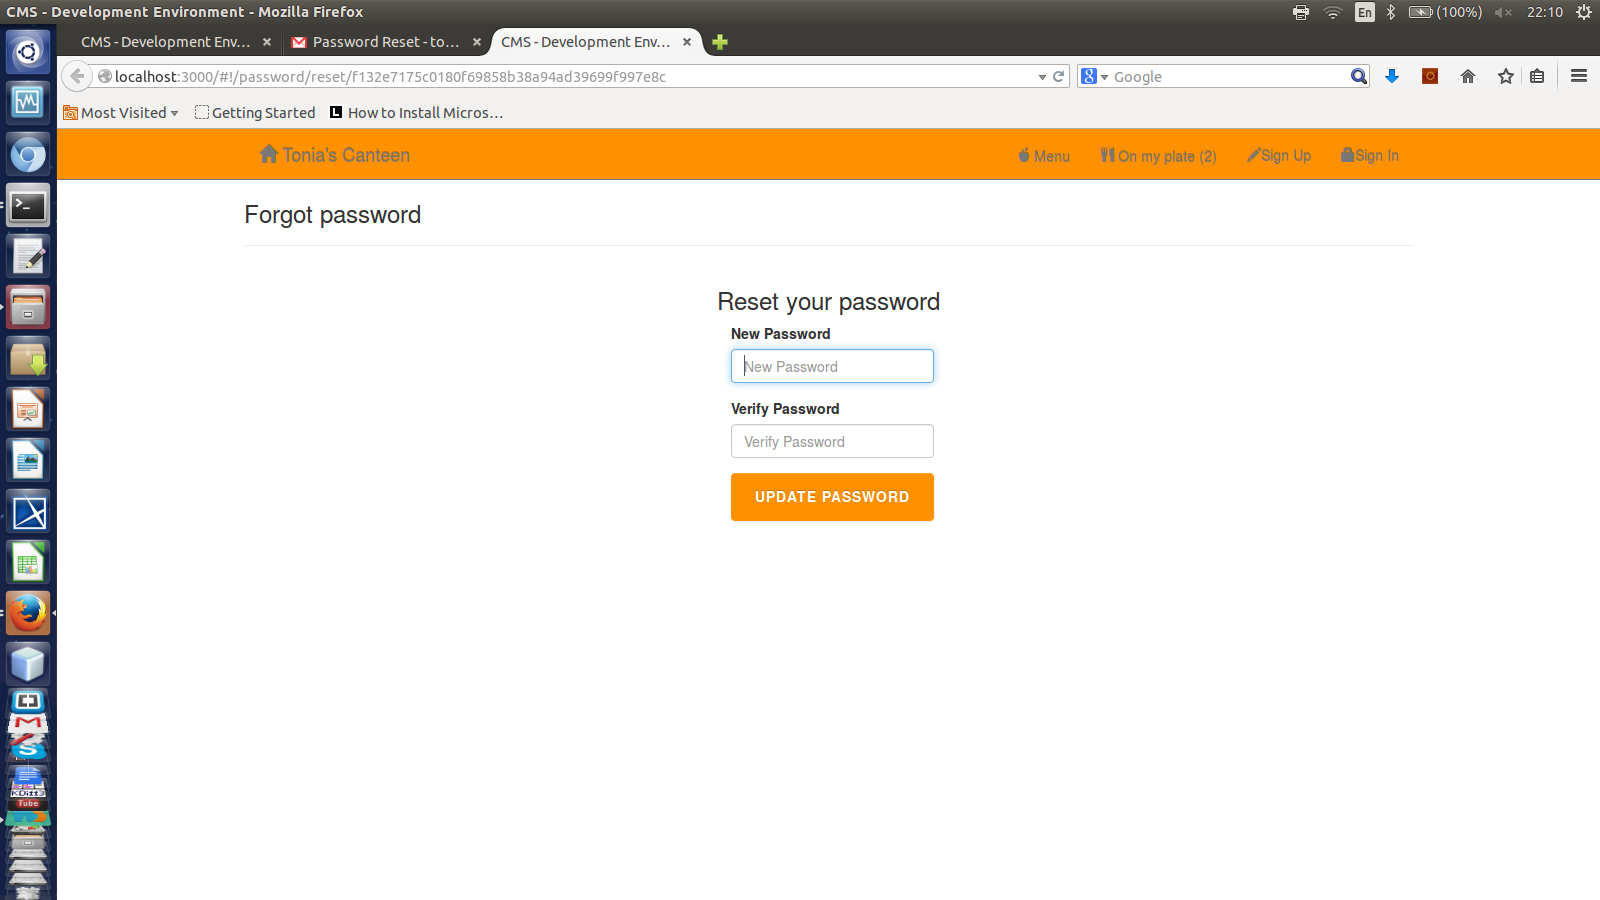
\includegraphics[width=1.0\textwidth]{screenshots/newPassForPass.png}
    \caption{The url sent via email leads to this page - fill in the textboxes and new password is set} 
\end{figure}


%%-------------------------------------USING THE SYSTEM----------------------------------------
\section{Using The System} 

%%------------------------NAVIGATION PANE ----------------------
\subsection{The Navigation pane} 

%%------------------------NAVIGATION PANE USER  NOT LOGGED ON ----------------------
\subsubsection{The Navigation pane - once the user is not  logged on}
On the home page, the name of the canteen is displayed. There is a navigation pane located at the top of the screen. The options available on the pane are "Sign in", "Sign up", "Menu" and "On your plate" and "Contact Us". 
The Navigation pane will be displayed as follows if the user has not logged in:

\begin{figure}[H]
  \centering
    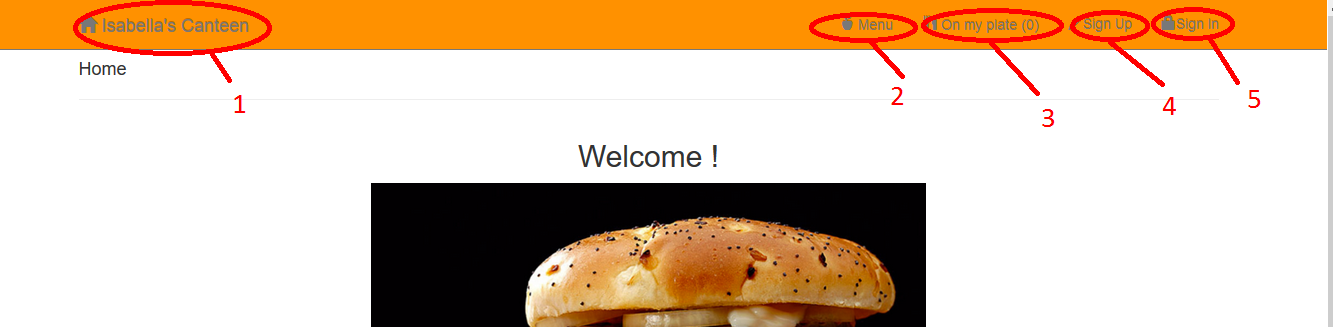
\includegraphics[width=1.0\textwidth]{screenshots/HomePage.png}
    \caption{Home Page - user has not logged in } 
\end{figure}

%%The numbers in the images are described below: -- CAN NUMBERS BE ADDED TO THE NEW SCREENSHOT?
The options on the navigation pane are described below:
\begin{enumerate}
\item Home -  when clicked, one will be redirected to the home page
\item Menu - when clicked, this will direct user to the menu page
\item On my plate -  when clicked, the user will be to an orders page showing items you have currently ordered and the bill total
\item Contact Us - when clicked, it directs the user to a page that contains the contact details of the canteen 
\item Sign Up - this button will direct to the signup page where a new account can be created
\item Sign In - this button will direct to a page where the user can signin and log into his/her account
\end{enumerate}

The user cannot proceed to order food if the user has not signed up and logged in. Hence, the first step a new user should take is signing up/ registering with the system. 
\\ \\
If a user has not signed in, the user will still be allowed, however, to view the menu, without ordering anything. However, the user will be able to add items to their plate and view them on the "On My Plate" page, but the order will not be sent to the system until the user signs in.


%%------------------------NAVIGATION PANE USER LOGGED ON  ----------------------
\subsubsection{The Navigation pane - once the user has logged on}
Once the user has logged on, the options that will be available on the navigation pane are  "Menu", "On your plate", "Contact Us" and a dropdown menu labelled with the users name and surname. Various options are displayed on this dropdown menu depending on the type of the user. If the user is a normal user the following items will be displayed on the dropdown, "Notifications", "View Profile","Edit Profile", "My History","Change Password", "Sign out". These pages will be discussed below.

\begin{figure}[H]
  \centering
    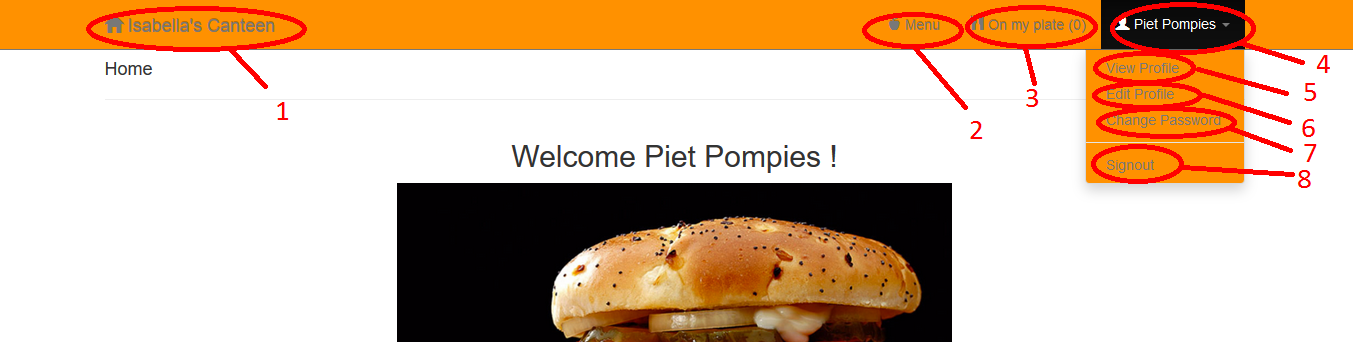
\includegraphics[width=1.0\textwidth]{screenshots/HomePage2.png}
    \caption{Home Page - user has logged in } 
\end{figure}


When a user is logged in as a normal user he/she will view of the navigation pane as indicated in the figure above.\\ below we describe the purpose of each of those options: \\

\begin{enumerate}
\item Home -  when clicked, one will be redirected to the home page
\item Menu - when clicked, this will direct user to the menu page
\item On my plate -  when clicked, the user will be to an orders page showing items you have currently ordered and the bill total
\item Contact Us - when clicked, it directs the user to a page that contains the contact details of the canteen 
\item The dropdown menu - when clicked, this will launch a dropdown menu with different options depending on the type of user - the example used is just a standard user with the basic options. These are described below:
\item Notifications -  when clicked, this will redirect the user to a page that displays various system notifications. A number next to the "Notifications" label on the dropdown menu will indicate the number of new unread notifications that have been sent to the user.
\item View Profile - when clicked, this will redirect to the profile page of the respective user.
\item Edit Profile - when clicked, this will redirect to the edit profile page where a user can change his/her current details and save it onto the CMS
\item My History - when clicked the user will be directed to page where the user can view a tabular and graphical version of their spending history for the month.
\item Change Password - when clicked, this will redirect to the change password page where a user can change his/her current password
\item Sign Out  - this will sign a user out of the CMS and redirect the user to the home page
\end{enumerate}

\textbf{Normal User}\\
A normal user will only have the options in the dropdown menu as displayed in the image above. If the user obtains another role, there will be extra settings displaying in the dropdown menu. \\

\textbf{Superuser or Admin User}\\
If the user is a superuser or an admin user the options "Admin Settings", "Audits" and "Branding Settings" will also be displayed in the dropdown menu. The superuser and the admin user will be in charge of assigning roles, changing employee ID's, removing employees, setting the system wide spending limit, changing the canteen name, theme and the carousel images of the canteen.  \\

\begin{figure}[H]
  \centering
    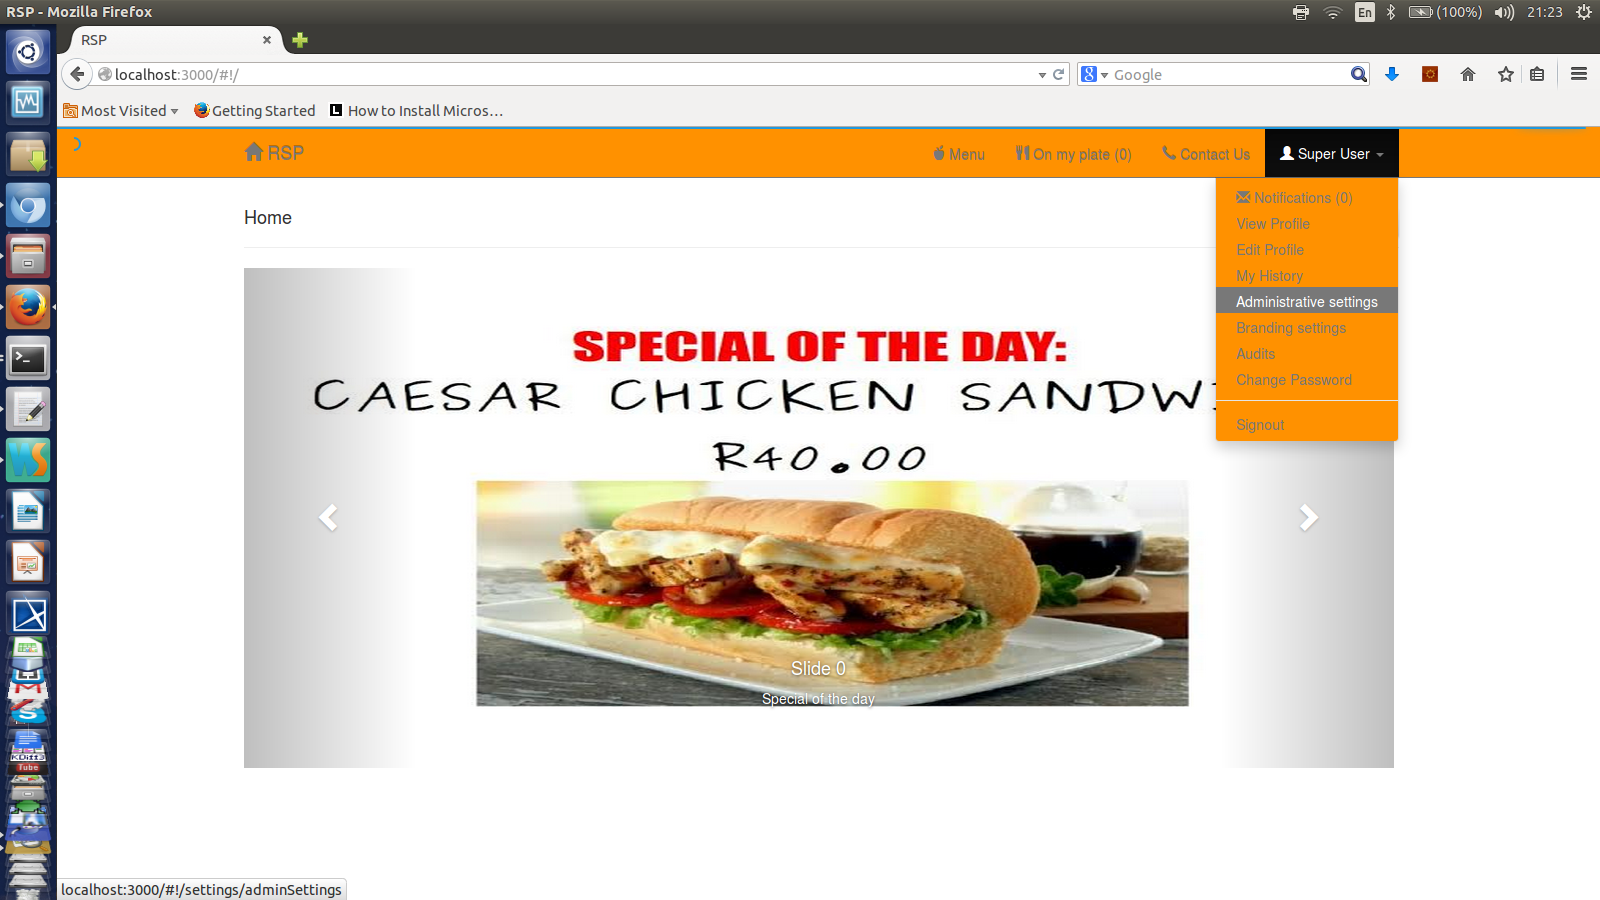
\includegraphics[width=1.0\textwidth]{screenshots/superUserMenu.png}
    \caption{The dropdown menu as per the superuser page} 
\end{figure}


\textbf{Cafeteria Manager}\\
If the user is a cafeteria manager, the options "Manage Menu", "Manage Inventory", "Menu items statistics", "Inventory statistics" will be displayed. Manage Inventory is where the stock additions and removals are kept track of. Manage Menu Items  is where the different menu meal items will be logged. The statistics pages will display graphical representations of the most popular items and of the items sold\\

\begin{figure}[H]
  \centering
    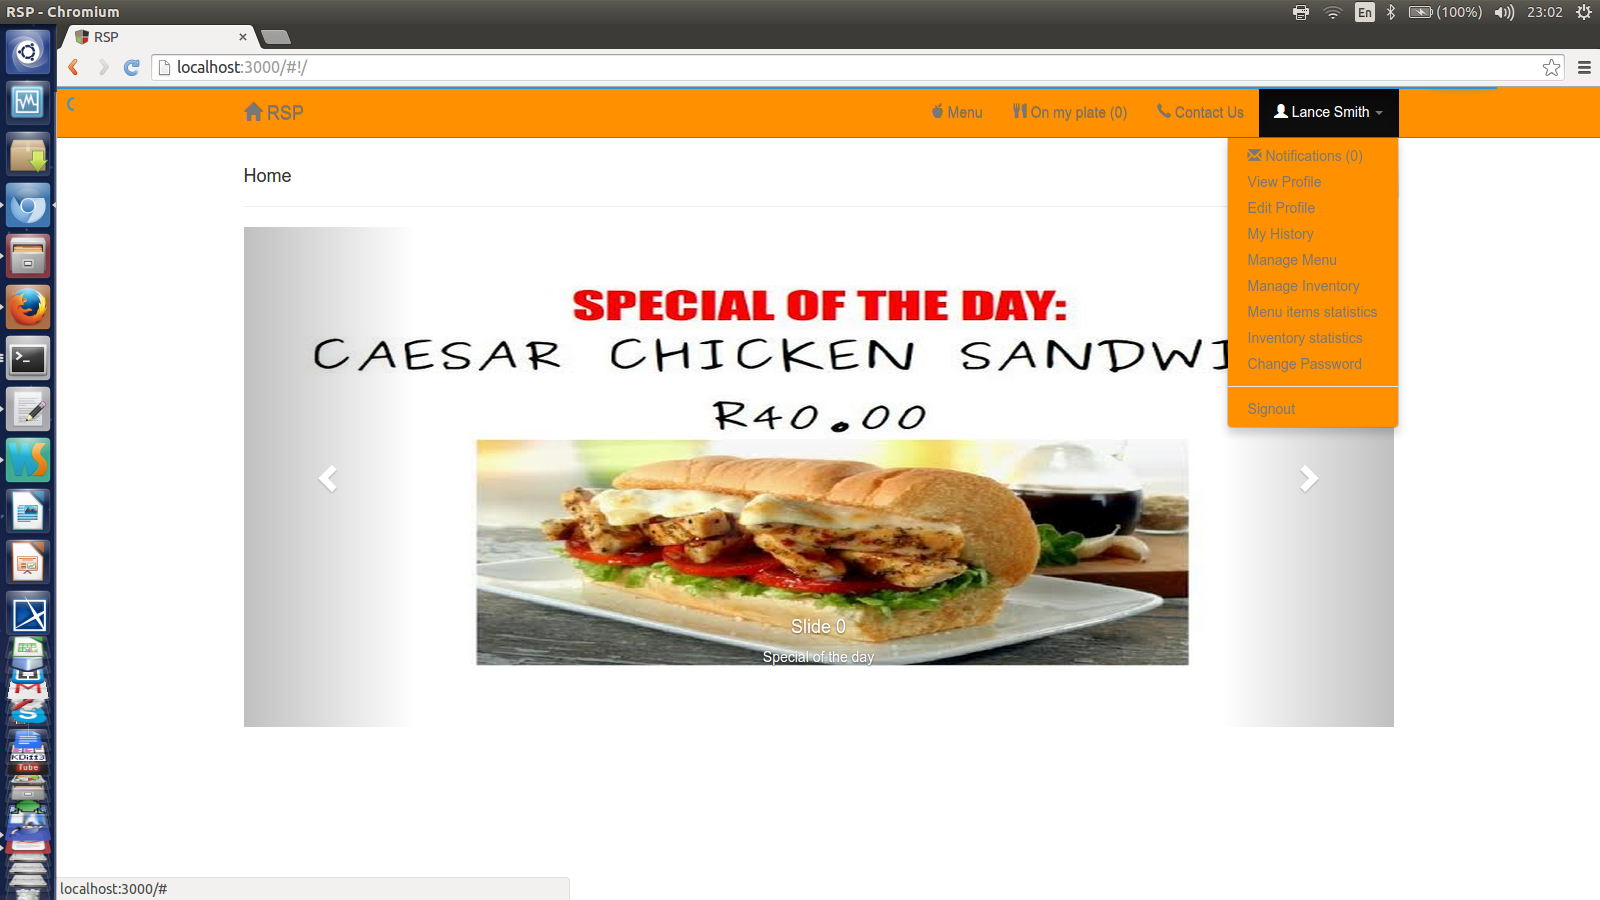
\includegraphics[width=1.0\textwidth]{screenshots/cafeteriaMenu.png}
    \caption{The dropdown menu as per the cafeteria page} 
\end{figure}

\textbf{Finance}\\
If user is a financial manager, the option "View Employee Bills" will be displayed. The financial manager will be able to search for employees and view their bills for a configurable period of time.\\

\begin{figure}[H]
  \centering
    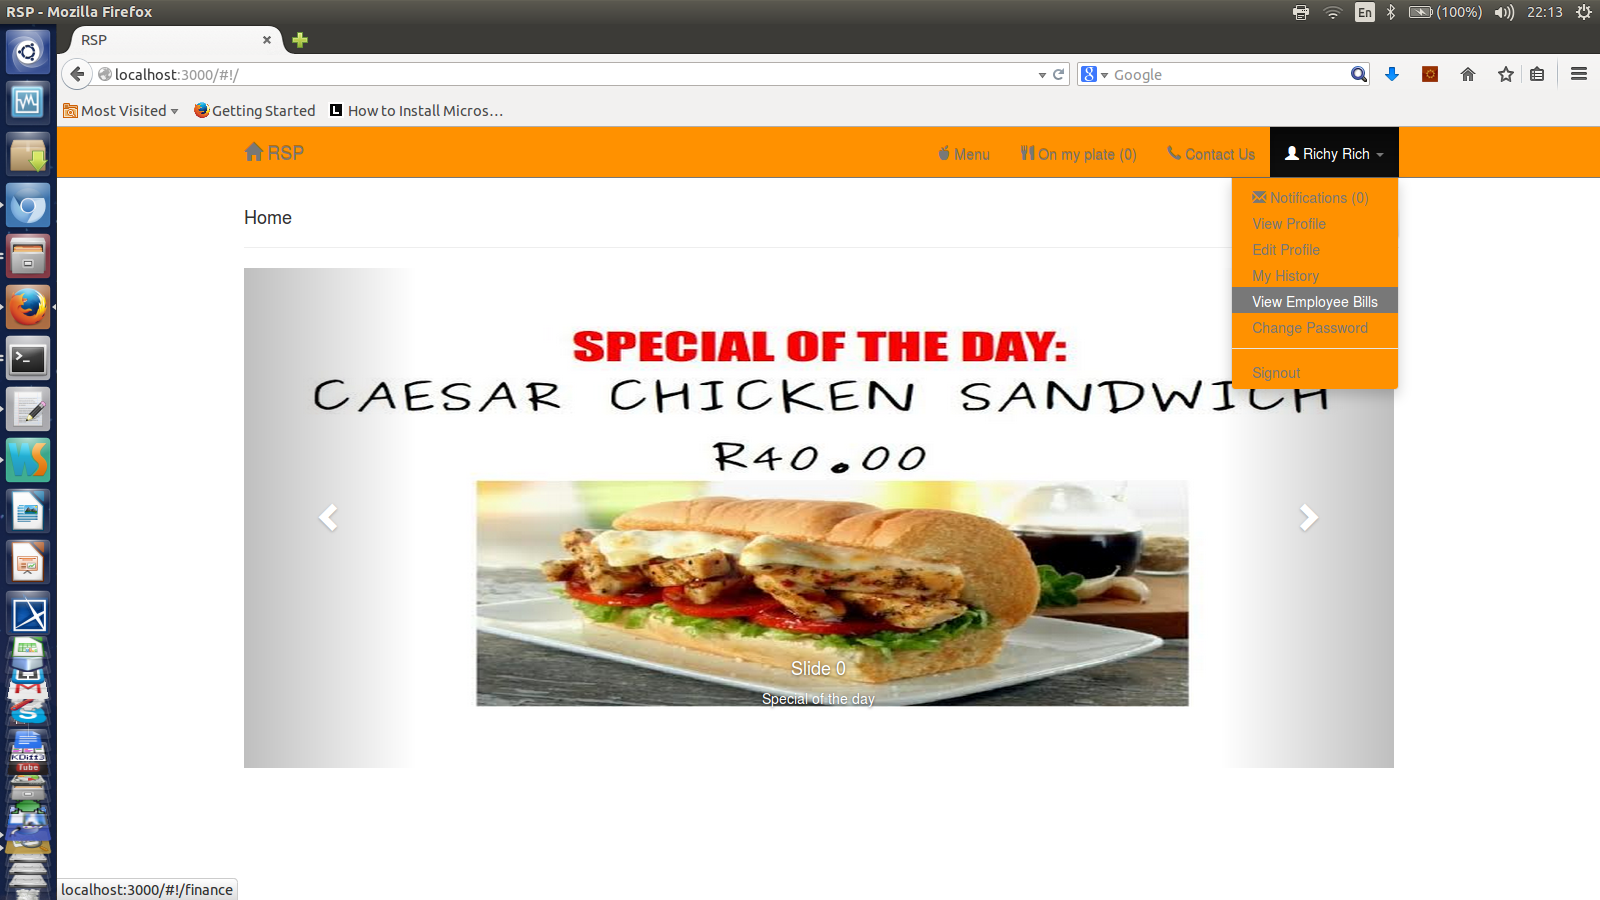
\includegraphics[width=1.0\textwidth]{screenshots/financeMenu.png}
    \caption{The dropdown menu as per the cafeteria page} 
\end{figure}

\textbf{Cashier}\\
If the user is a cashier, the options "Process Orders" will be displayed and it is here where the transactions will occur, such as marking whether orders are ready, and paid for. When the "Order ready" is clicked, notifications are sent to the user via email and via the notifications page, alerting the user that his/her order is ready for collection. 
\begin{figure}[H]
  \centering
    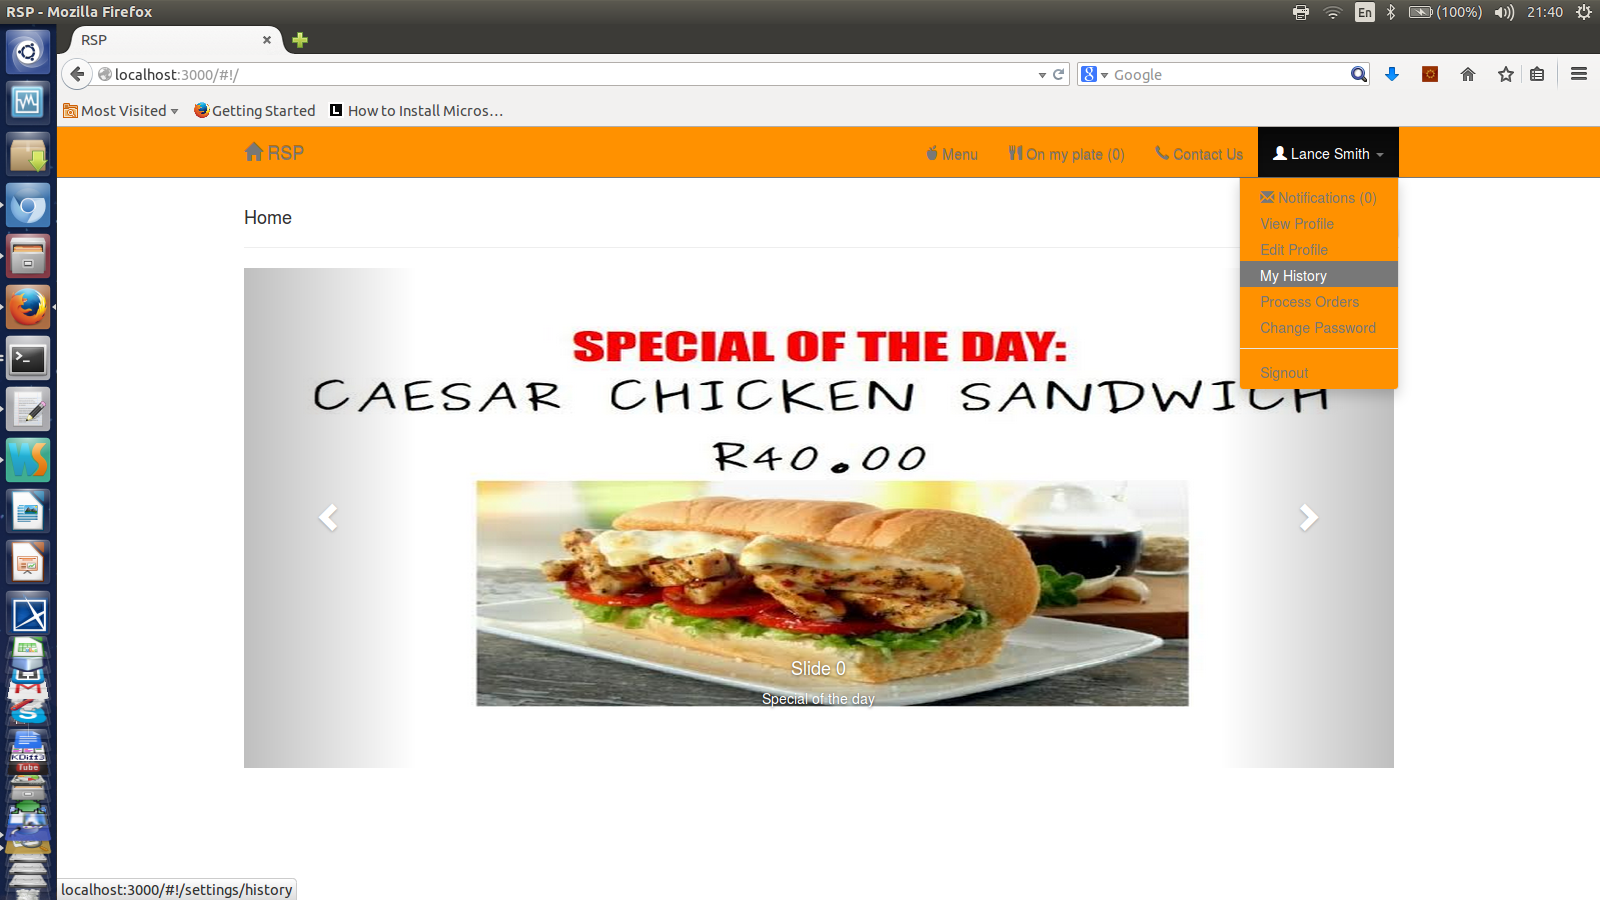
\includegraphics[width=1.0\textwidth]{screenshots/cashierMenu.png}
    \caption{The dropdown menu as per the cafeteria page} 
\end{figure}

%%------------------------MENU PAGE----------------------
\subsection{The "Menu" Page} 
This is where the user will be able to view the menu items and their prices. An item can be added to the user's plate by simply clicking the 'Add to Plate' button alongside each item. These can then be viewed on the 'On my Plate' page.
If a menu item is not in stock it will be written in red on the menu item that it is "out of stock " and there will be no  option to click the add to plate button since that item will not be available. 
\\
The image button displayed in each menu item field can be clicked to view images of the different menu items, as uploaded by the superuser.
\begin{figure}[H]
  \centering
    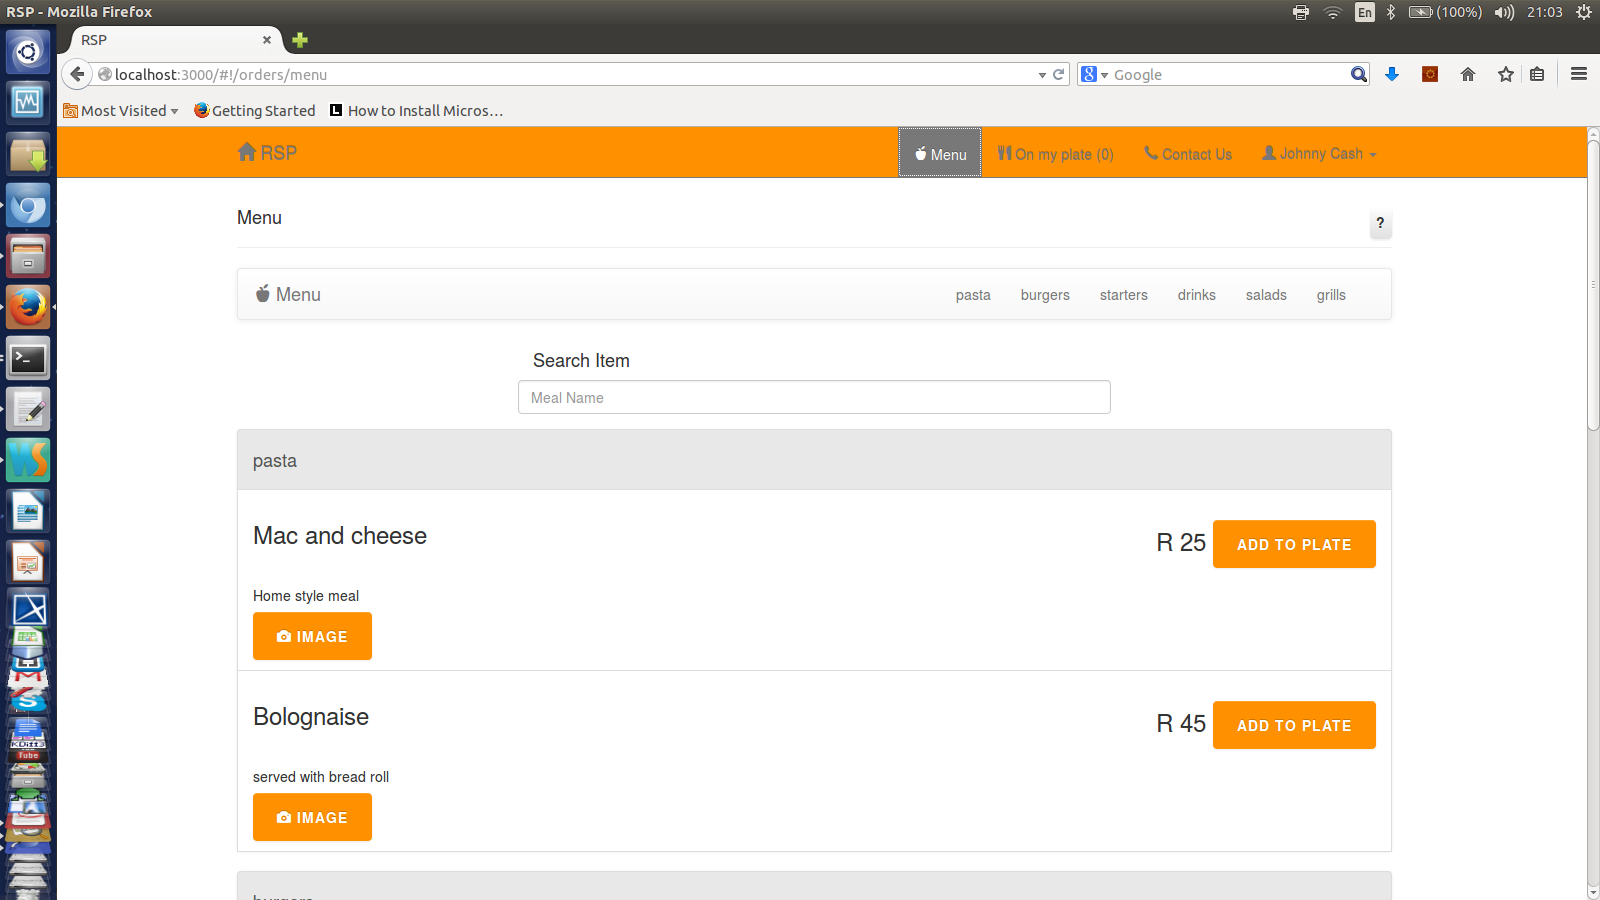
\includegraphics[width=1.0\textwidth]{screenshots/beforePasta.png}
    \caption{The menu page from which a user can order food} 
\end{figure}
On the menu page there is also a breadcrumb which indicates the different meal categories to make the search more efficient. There is also a search bar on all these pages. 

\begin{figure}[H]
  \centering
    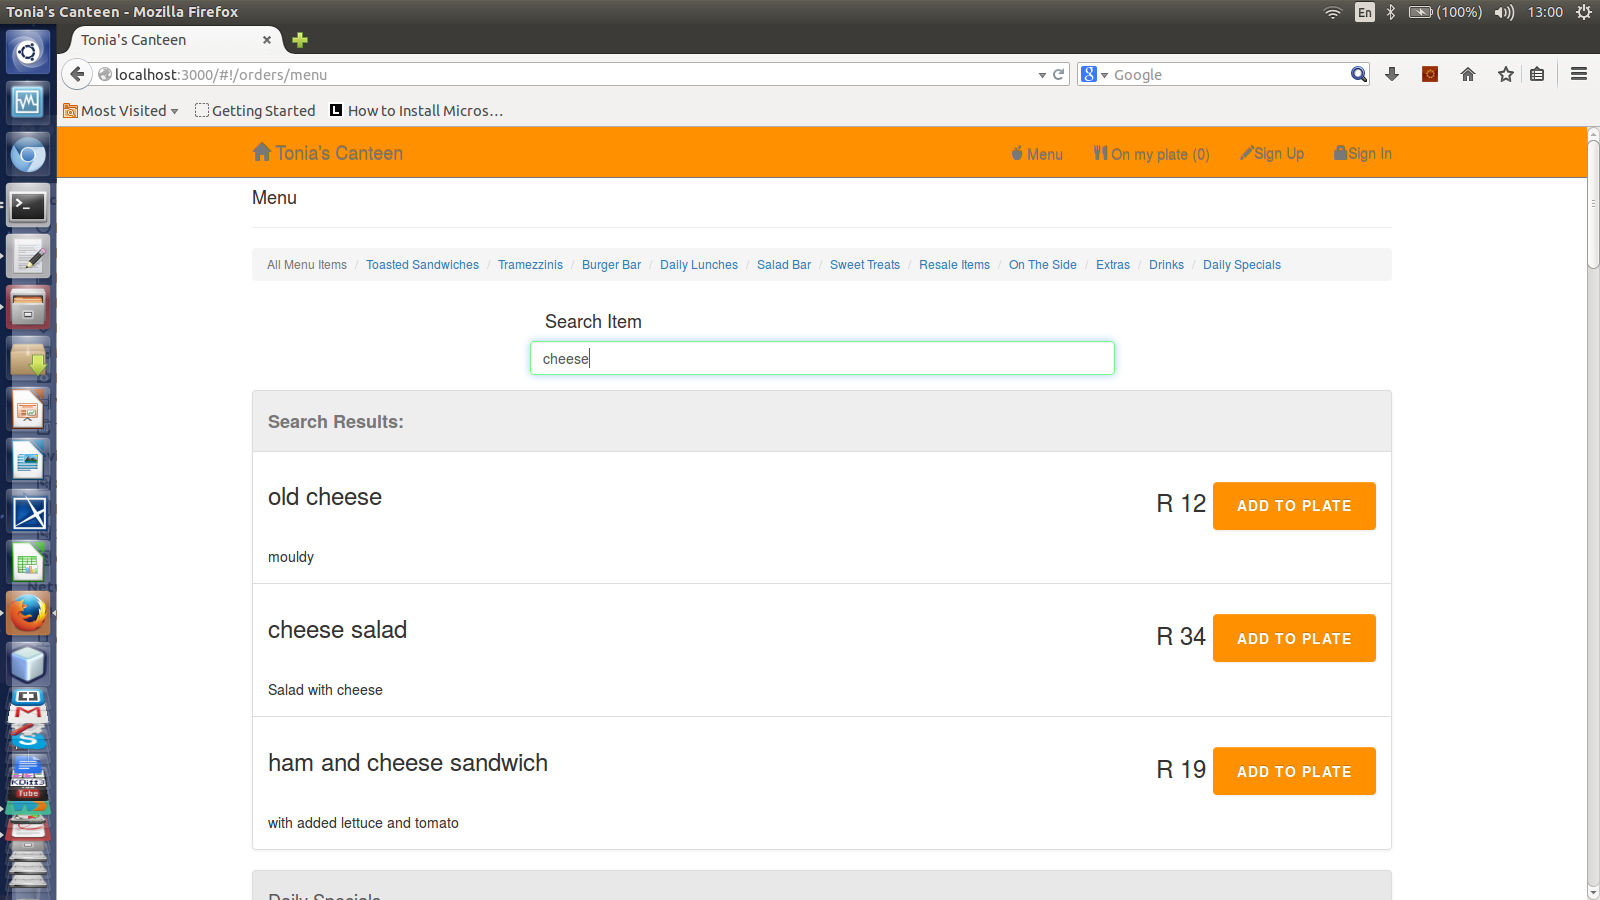
\includegraphics[width=1.0\textwidth]{screenshots/searchCheese.png}
    \caption{The menu page - Can be navigated via the search bar as illustrated} 
\end{figure}

\begin{figure}[H]
  \centering
    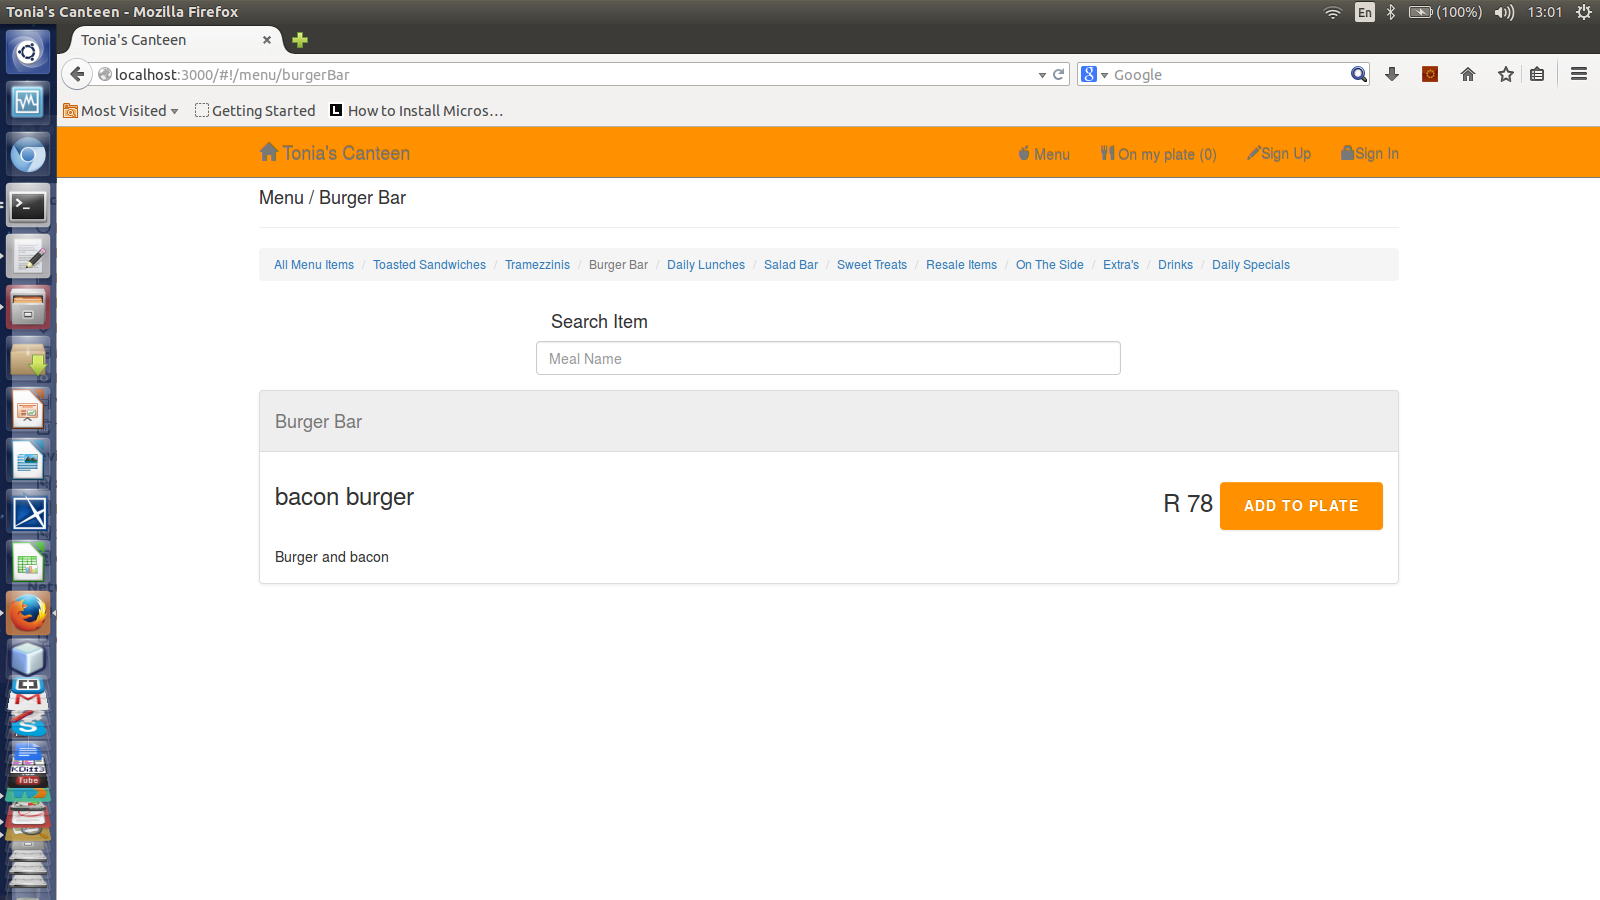
\includegraphics[width=1.0\textwidth]{screenshots/catMenu.png}
    \caption{The menu page - Can be navigated via the category breadcrumb as indicated to view sub menus} 
\end{figure}

\begin{figure}[H]
  \centering
    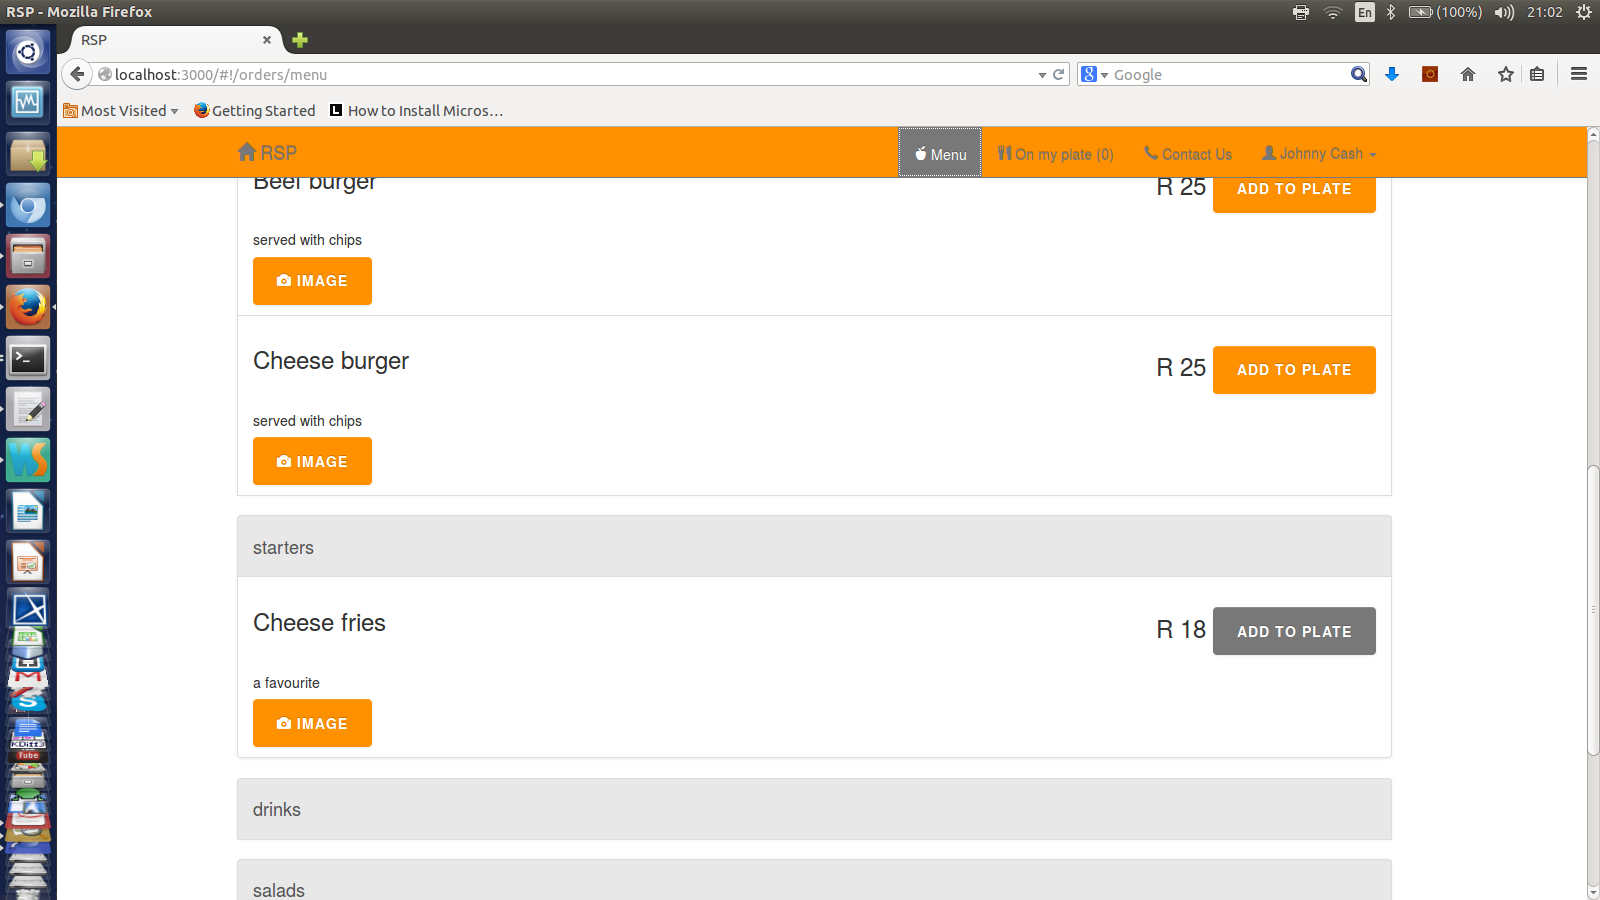
\includegraphics[width=1.0\textwidth]{screenshots/addToPlate.png}
    \caption{The menu page - order menu items by clicking the addToPlate button } 
\end{figure}

%%------------------------ON MY PLATE PAGE----------------------
\subsection{The "On my plate" Page} 
This page serves to indicate the current meal items that the user has on their plate. The user can also specify any preferences, if any, for each item on their plate, as well as the quantities of each item they wish to order. The total will dynamically increase/decrease accordingly when they add/remove items or change the quantities.

\begin{figure}[H]
  \centering
    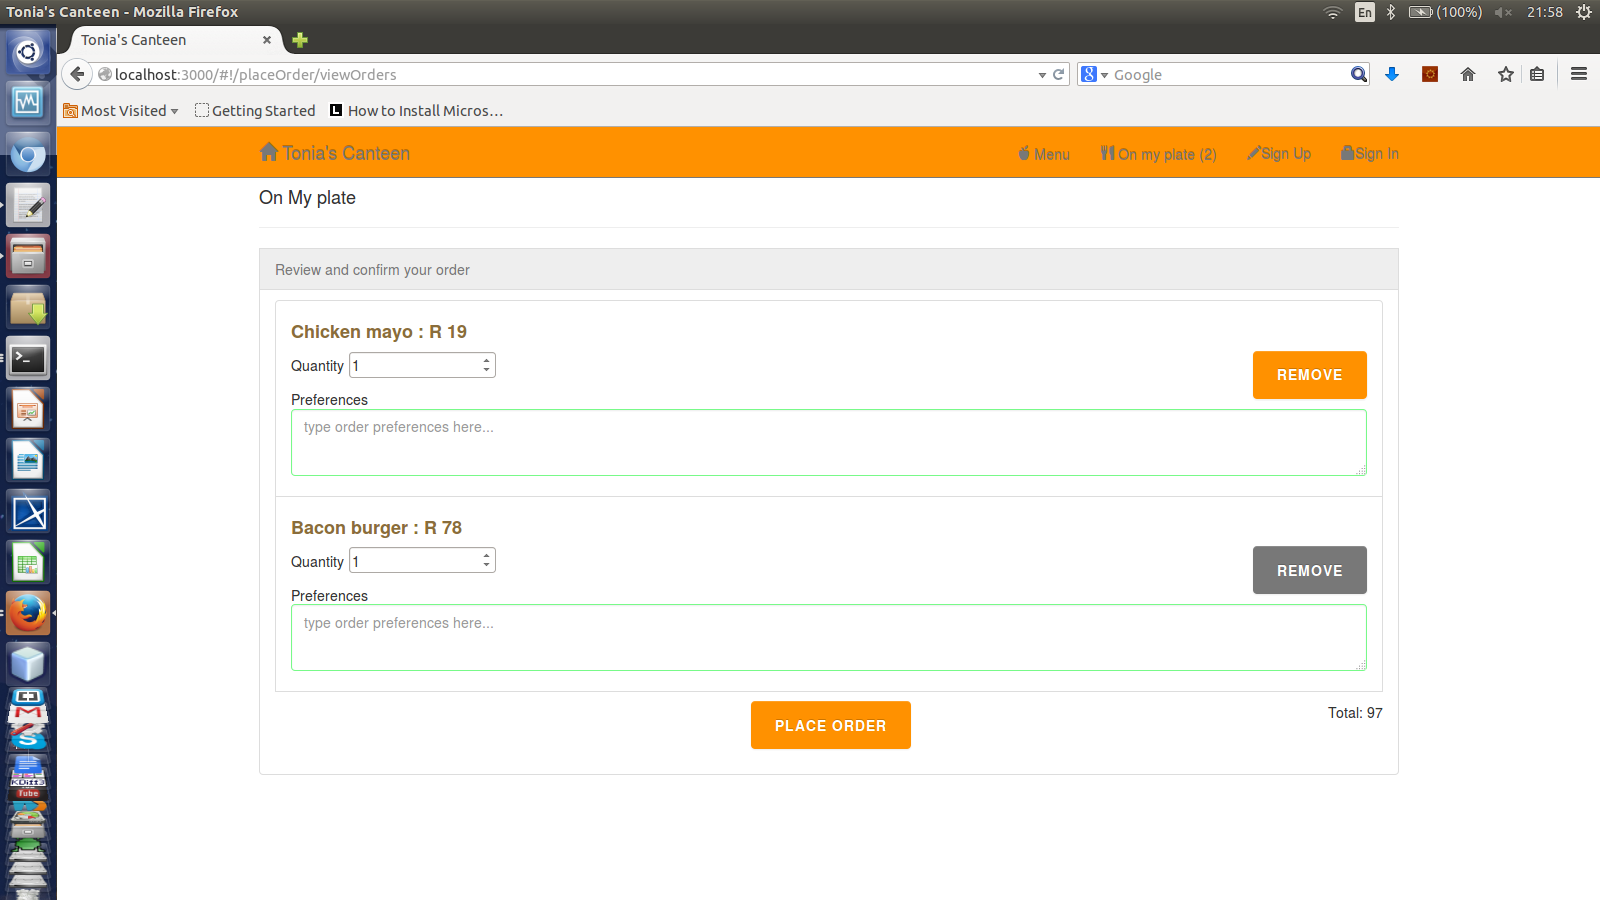
\includegraphics[width=1.0\textwidth]{screenshots/viewOrder1.png}
    \caption{On my plate page - The meal you selected on the menu page is displayed here (Navigate here via the navigation bar)} 
\end{figure}
\begin{figure}[H]
  \centering
    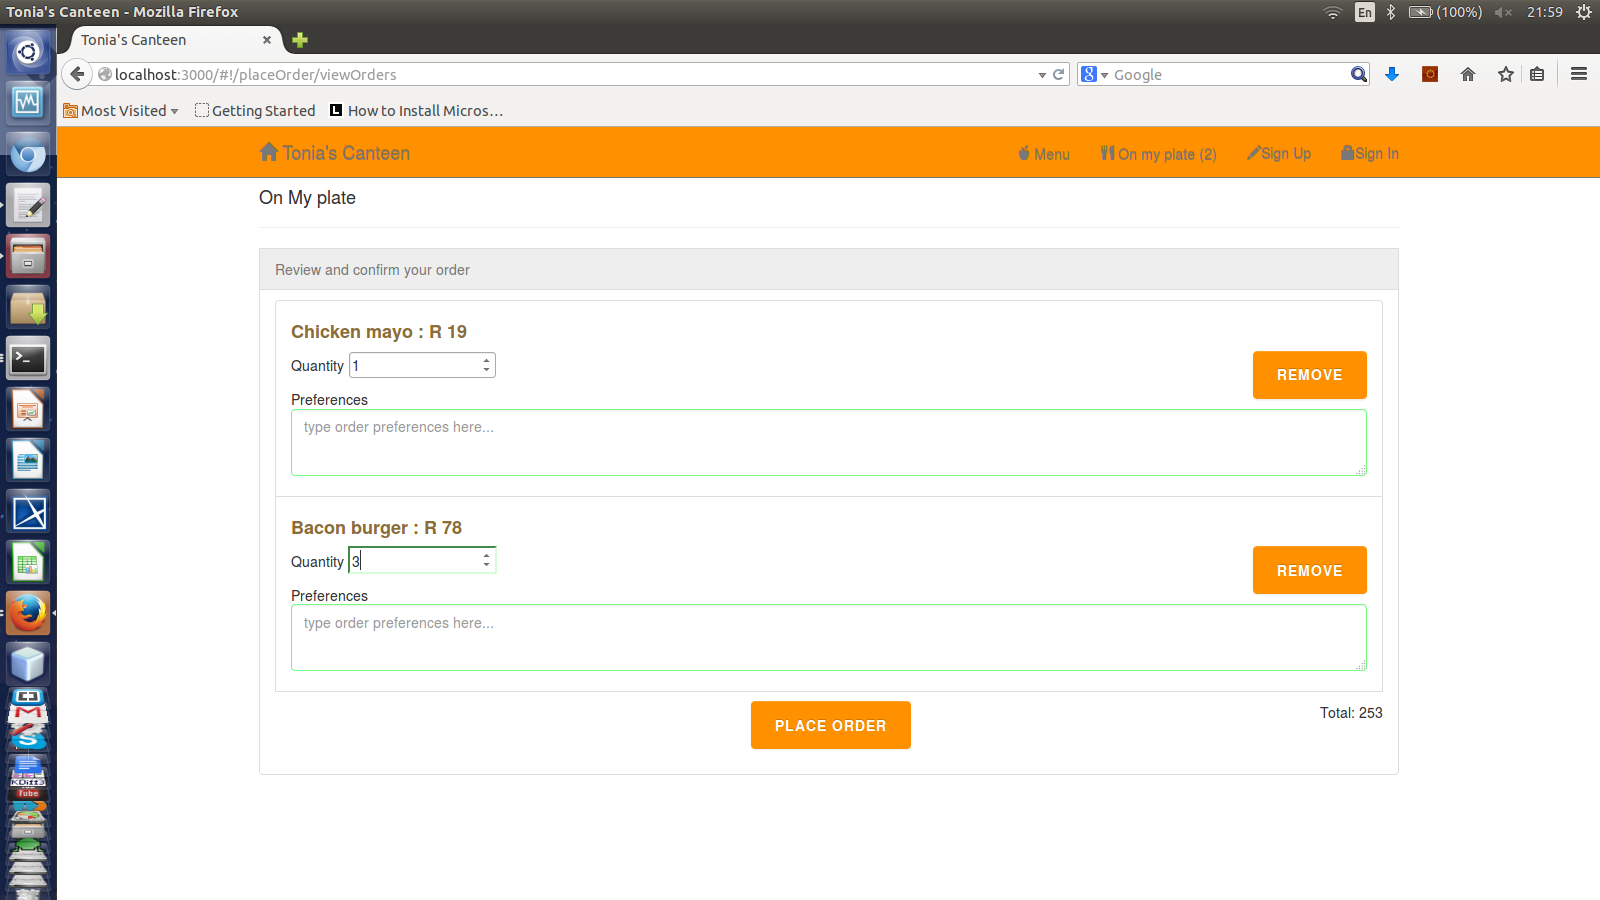
\includegraphics[width=1.0\textwidth]{screenshots/viewOrder2.png}
    \caption{One can increase the quantity of items ordered by editing the quantity field indicated} 
\end{figure}
\begin{figure}[H]
  \centering
    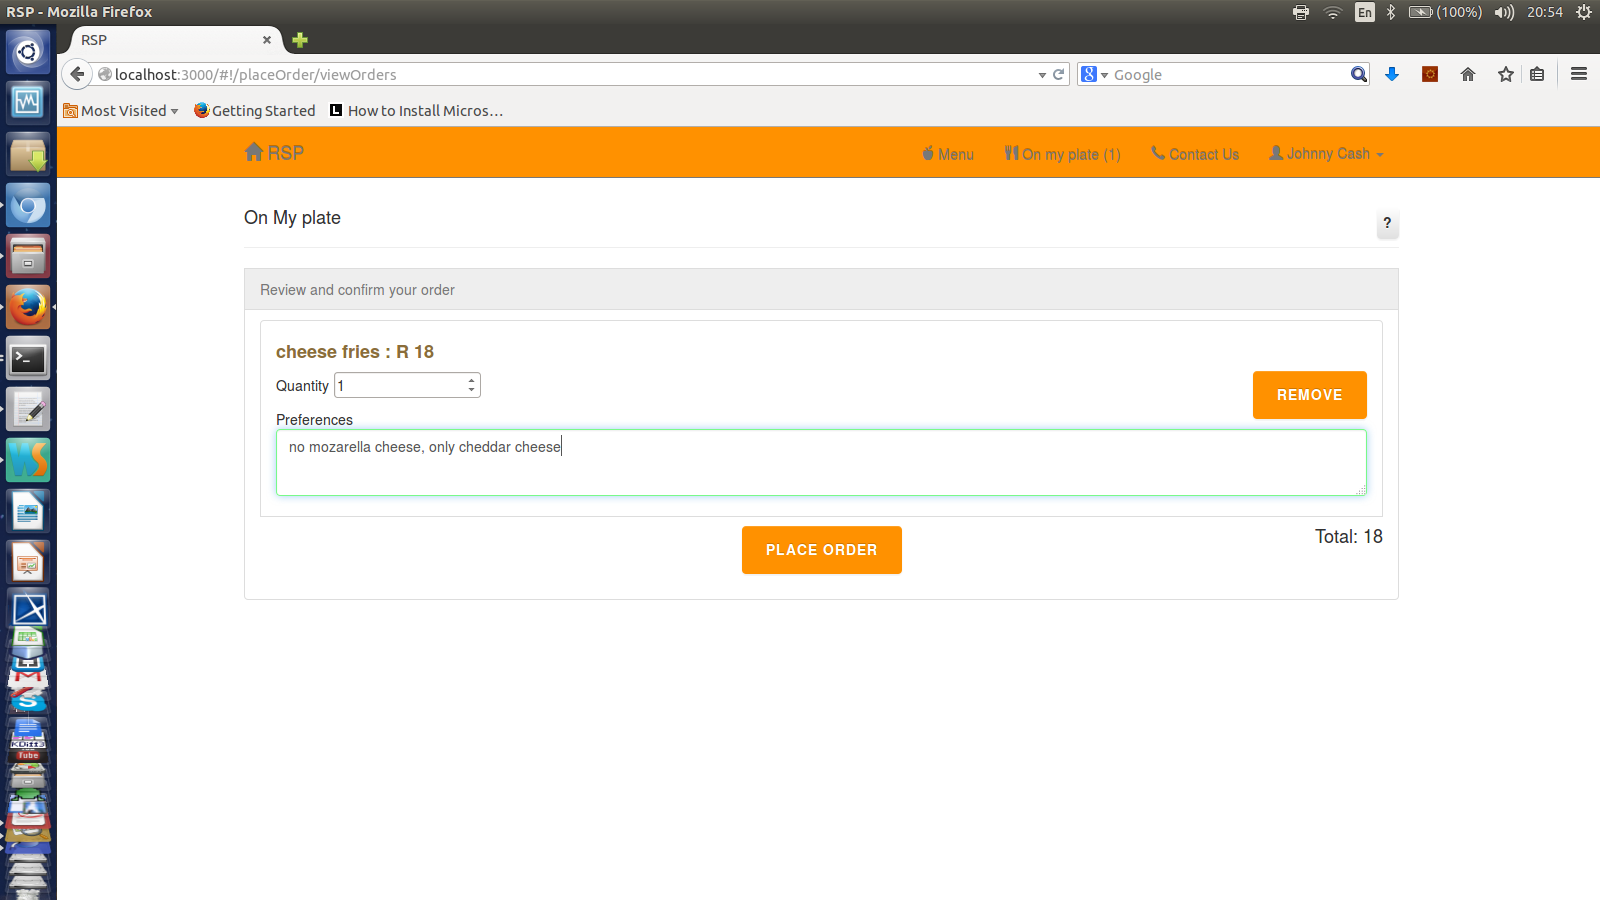
\includegraphics[width=1.0\textwidth]{screenshots/viewOrder3.png}
    \caption{One can remove orders as well as specify preferences by clicking in the indicated areas} 
\end{figure}

\subsection{The "Notifications" Page} 
When the user places an order, the user will recieve a notification informing the user that their order has indeed been placed. In addition, when a user places an order, the order is sent through to the cashier's page at the cafeteria. When the cashier is notified at the canteen that an order is ready for collection, the cashier will mark this order as ready and this will send a notification to the notification page.

\begin{figure}[H]
  \centering
    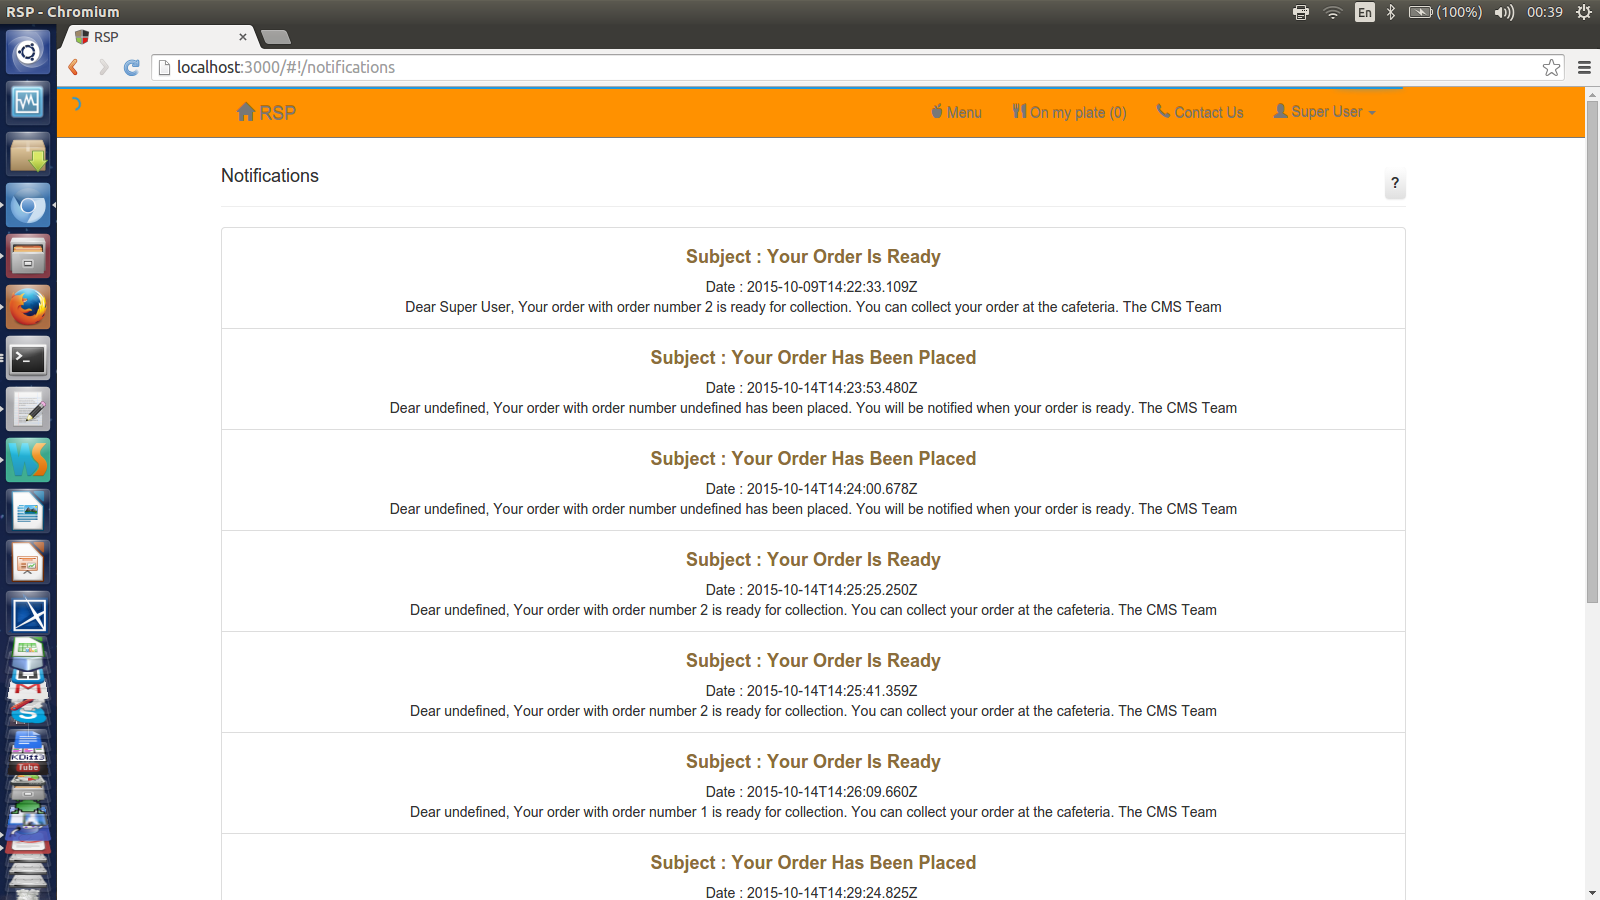
\includegraphics[width=1.0\textwidth]{screenshots/notifications.png}
    \caption{The notifications page -  consists of order pending and order ready notifications} 
\end{figure}


%%----------------------EDIT PROFILE PAGE ----------------------
\subsection{The "Edit Profile" Page} 
The user will be presented with a similar form to that which they signed up with, however, the details that the user entered in the signup form will be present in these textboxes. The user can proceed to edit these here. Clicking the submit button will indicate whether changes have been saved or if errors have been made and how the user can correct these.

\begin{figure}[H]
  \centering
    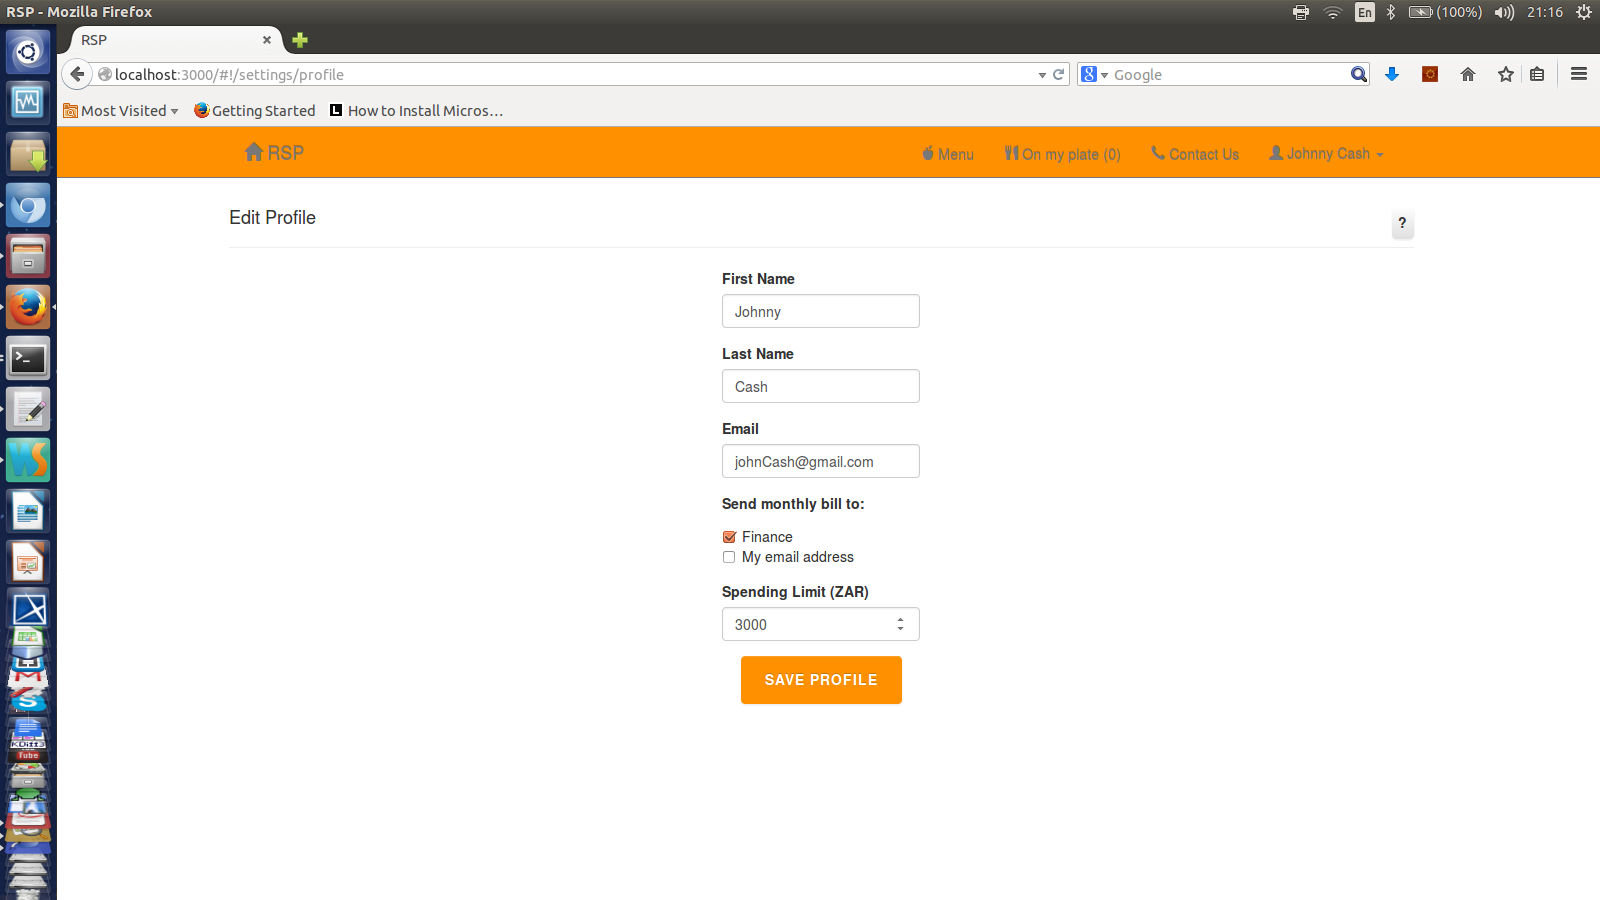
\includegraphics[width=1.0\textwidth]{screenshots/editProfile.png}
    \caption{Edit profile page - Edit profile by typing into the text boxes and submitting for validation message and to save new information } 
\end{figure}

\begin{figure}[H]
  \centering
    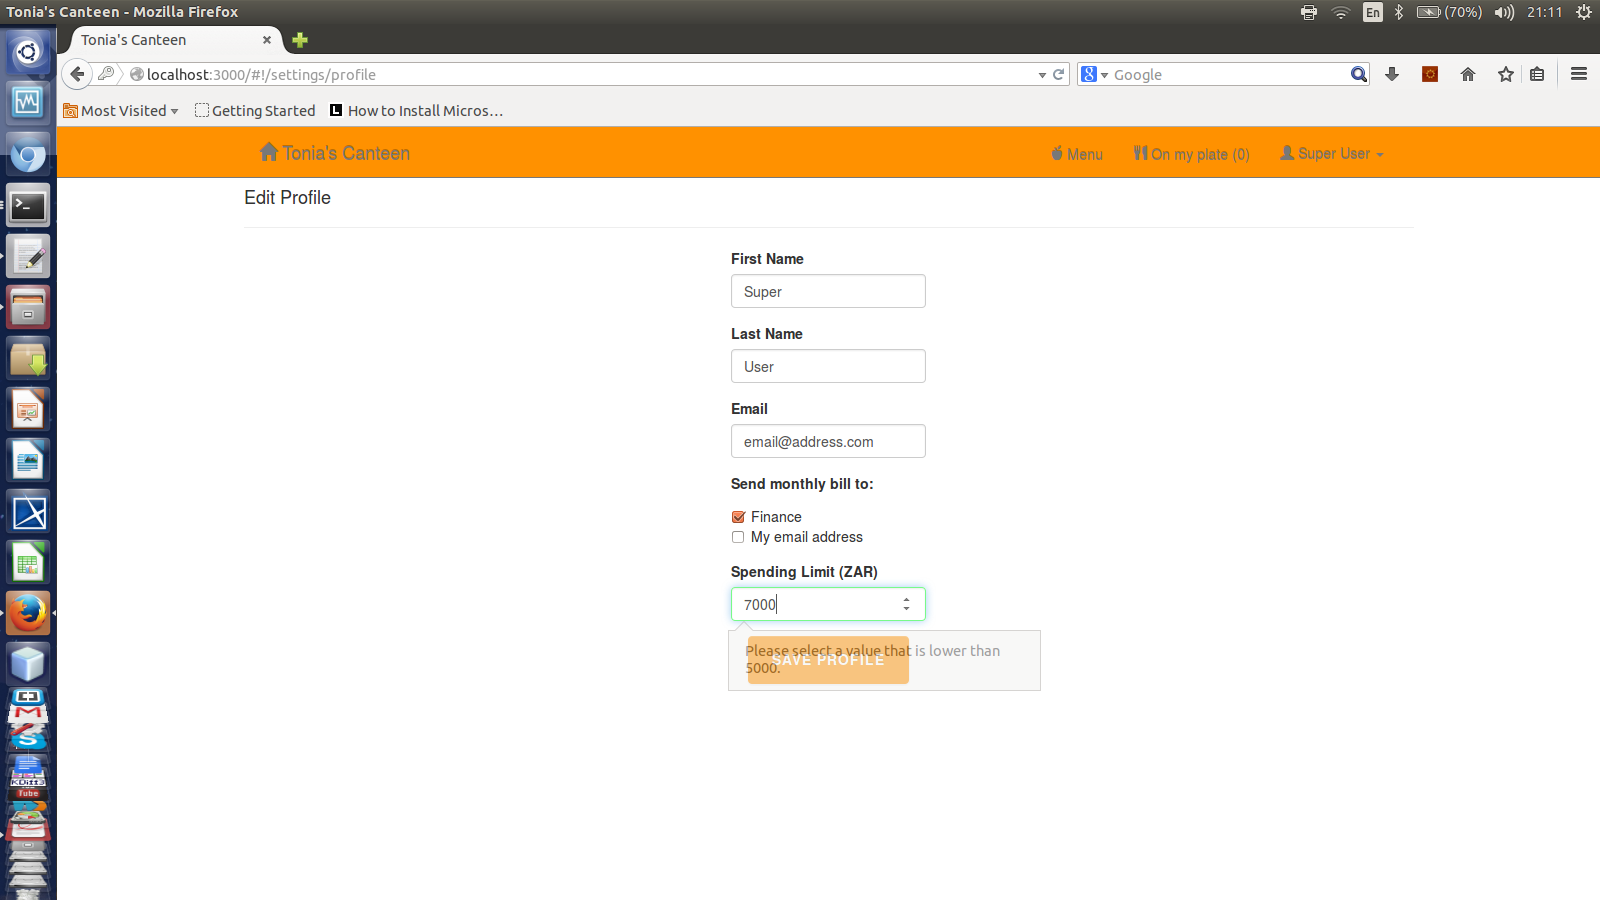
\includegraphics[width=1.0\textwidth]{screenshots/limitExeeds.png}
    \caption{You must ensure your monthly spending limit is within the bounds of the maximum spending limit of the system, set by the super user} 
\end{figure}

%%------------------------PROFILE PAGE----------------------
\subsection{The "Profile" Page} 
This is where the user will be able to view their profile i.e. the details they entered when they signed up/ edited their profile. 

\begin{figure}[H]
  \centering
    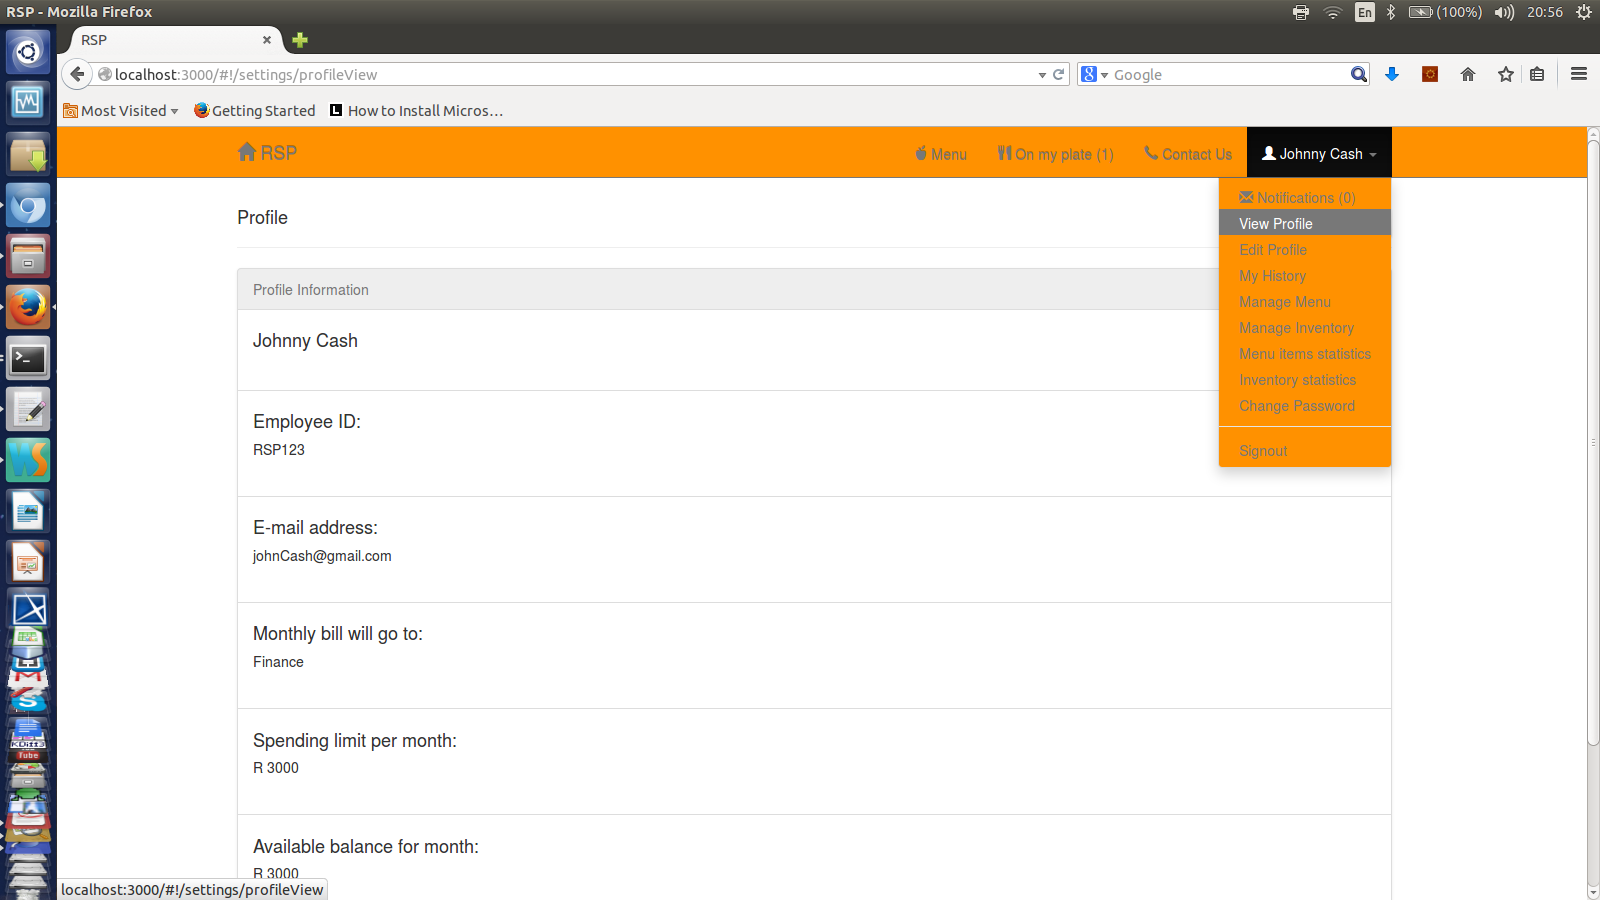
\includegraphics[width=1.0\textwidth]{screenshots/viewProfile.png}
    \caption{The profile page - where you view your profile (via the orange navigation tab menu indicated)} 
\end{figure}

%%-----------------------CHANGE PASSWORD PAGE----------------------
\subsection{The "Change Password" Page} 
The user is presented with a form where the user will be asked to enter their old and new passwords to change their password. 

\begin{figure}[H]
  \centering
    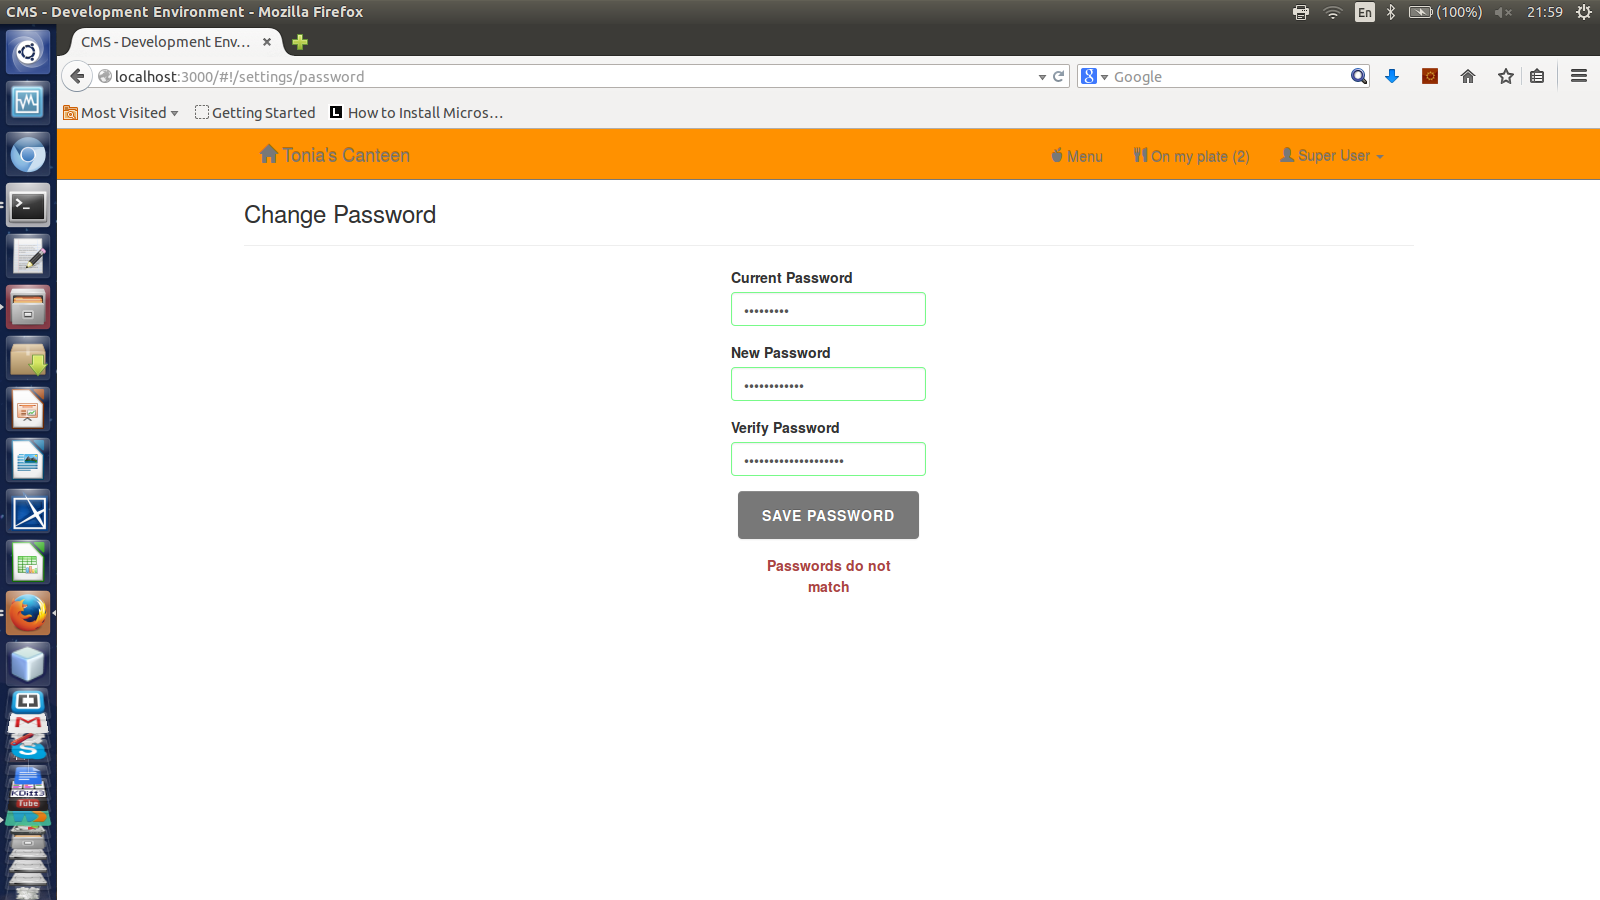
\includegraphics[width=1.0\textwidth]{screenshots/changePassDontMatch.png}
    \caption{Can change password on this page - validation message will be displayed indicating if change was successful or not} 
\end{figure}
%%-----------------------superuser admin ----------------------
\subsection{Superuser: The "Administrative Settings" Page} 
At the top of the page there is a section labelled assign roles, where different admin roles will be assigned to different users. The super user simply has to type in an employee ID and select a role from the dropdown menu below. There is a section underneath that where the superuser can change the user ID of an employee. Self explanatory text boxes are provided for the superuser to fill in and the submit button will save the changes, unless an error occurs.  This page also consists of a section labelled "Change system limit" and it is here where the superuser can alter the limit of the system, i.e. the maximum value that a user can set their daily spending limits to. Hence a textbox is provided for the super user to type the new limit and save it.  The superuser can also remove an employee from the system.
 
\begin{figure}[H]
  \centering
    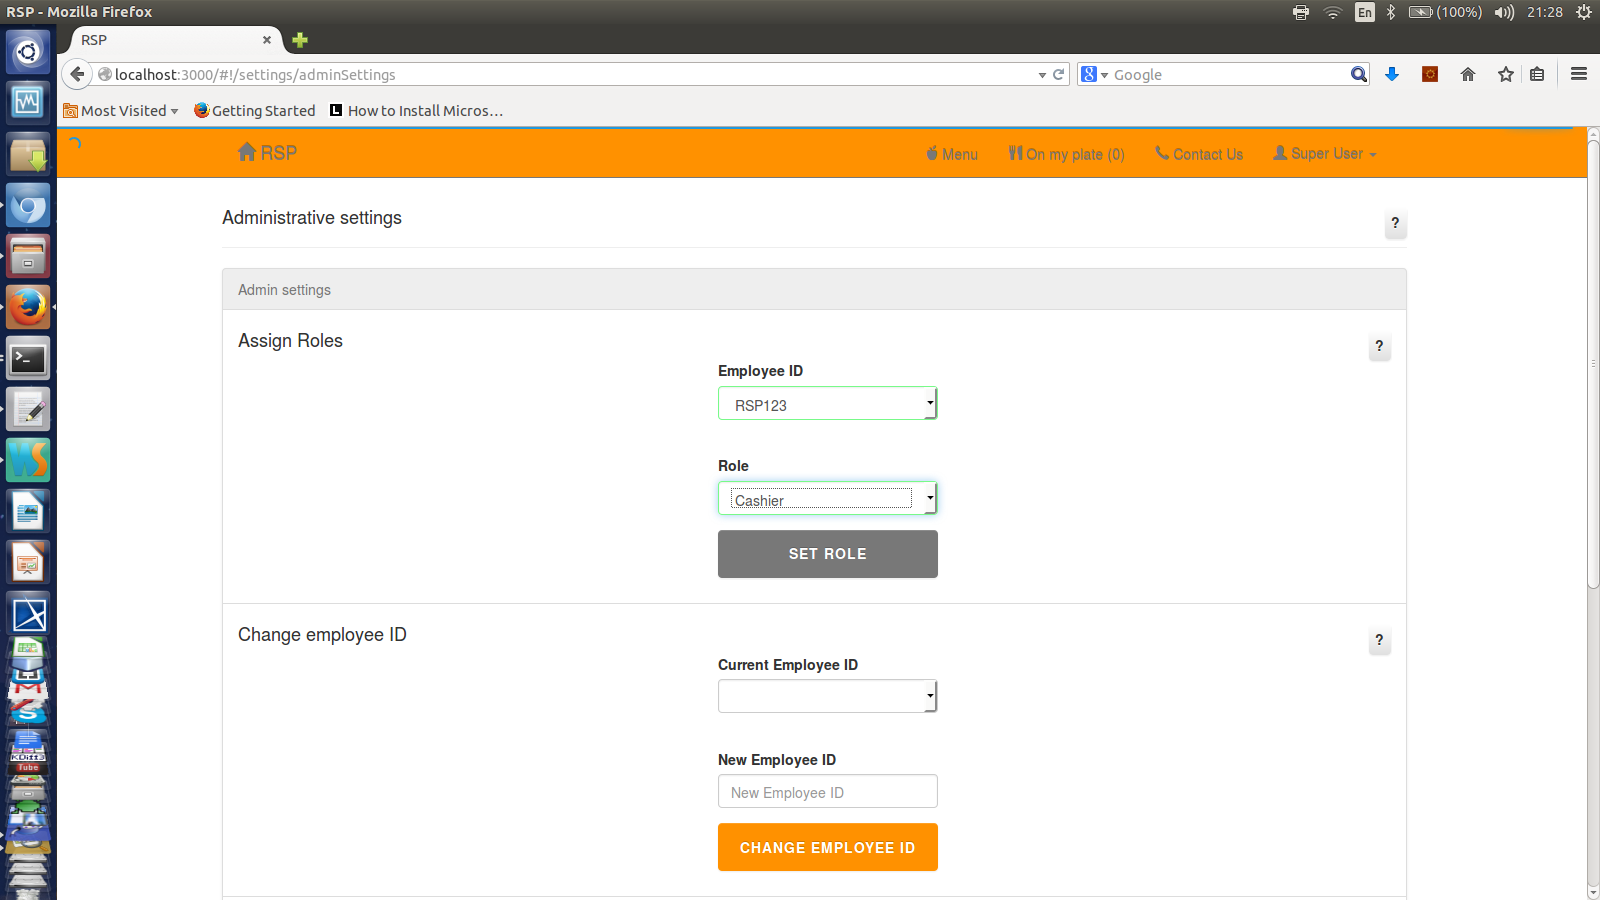
\includegraphics[width=1.0\textwidth]{screenshots/assignRole.png}
    \caption{The admin page - superuser can assign roles such as cashier to users} 
\end{figure}

\begin{figure}[H]
  \centering
    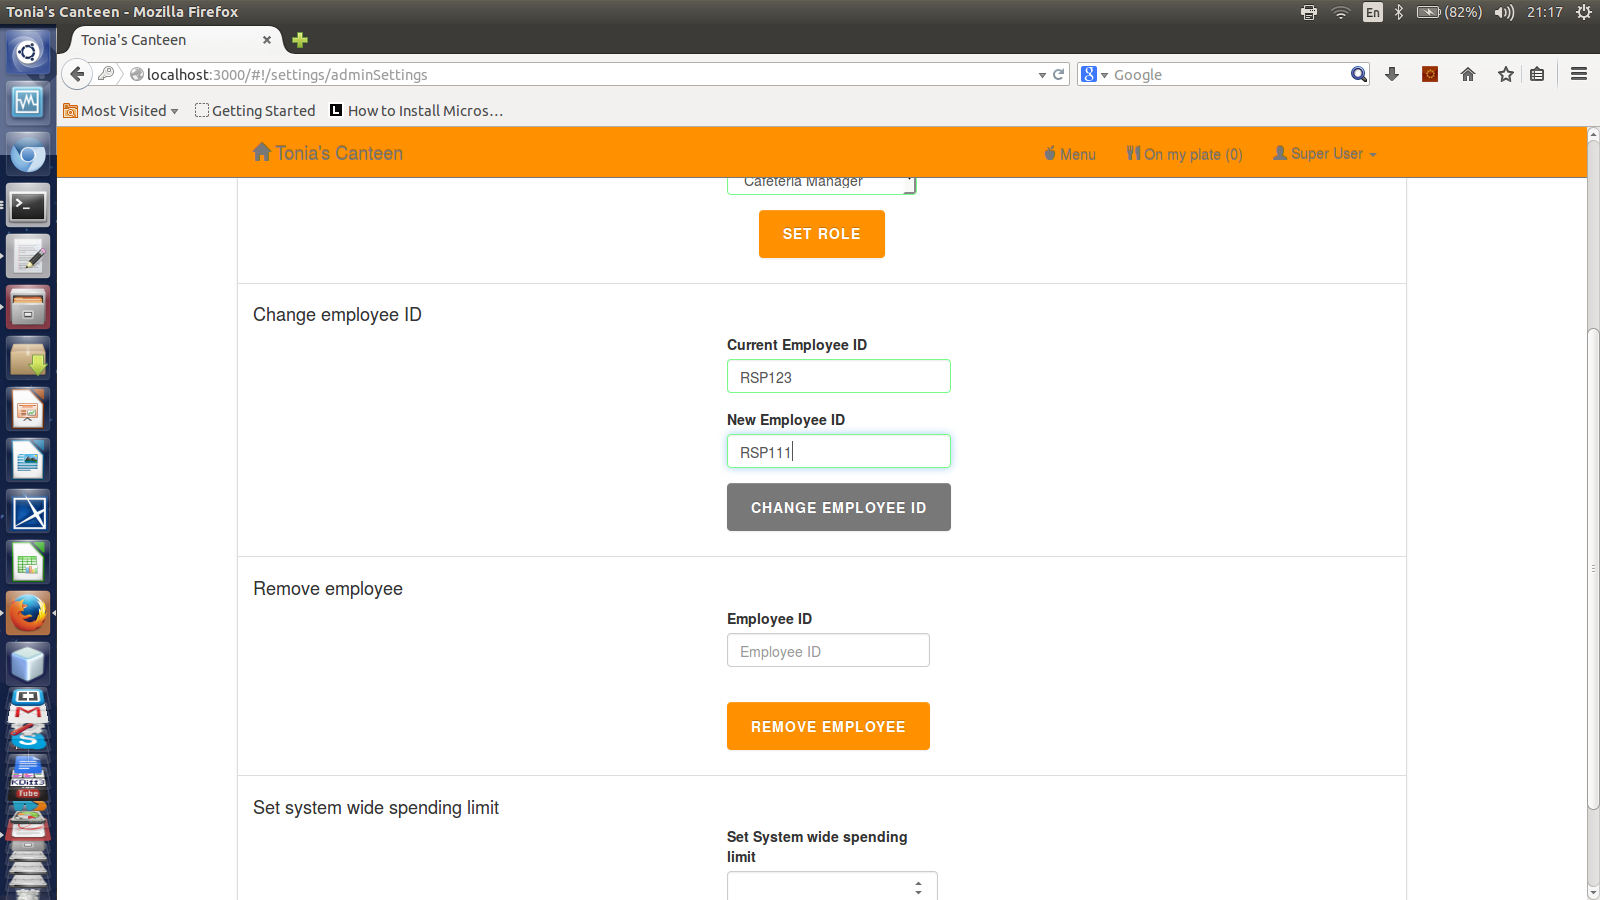
\includegraphics[width=1.0\textwidth]{screenshots/changeEmplid.png}
    \caption{The admin page - superuser can change the users' employee IDs} 
\end{figure}

\begin{figure}[H]
  \centering
    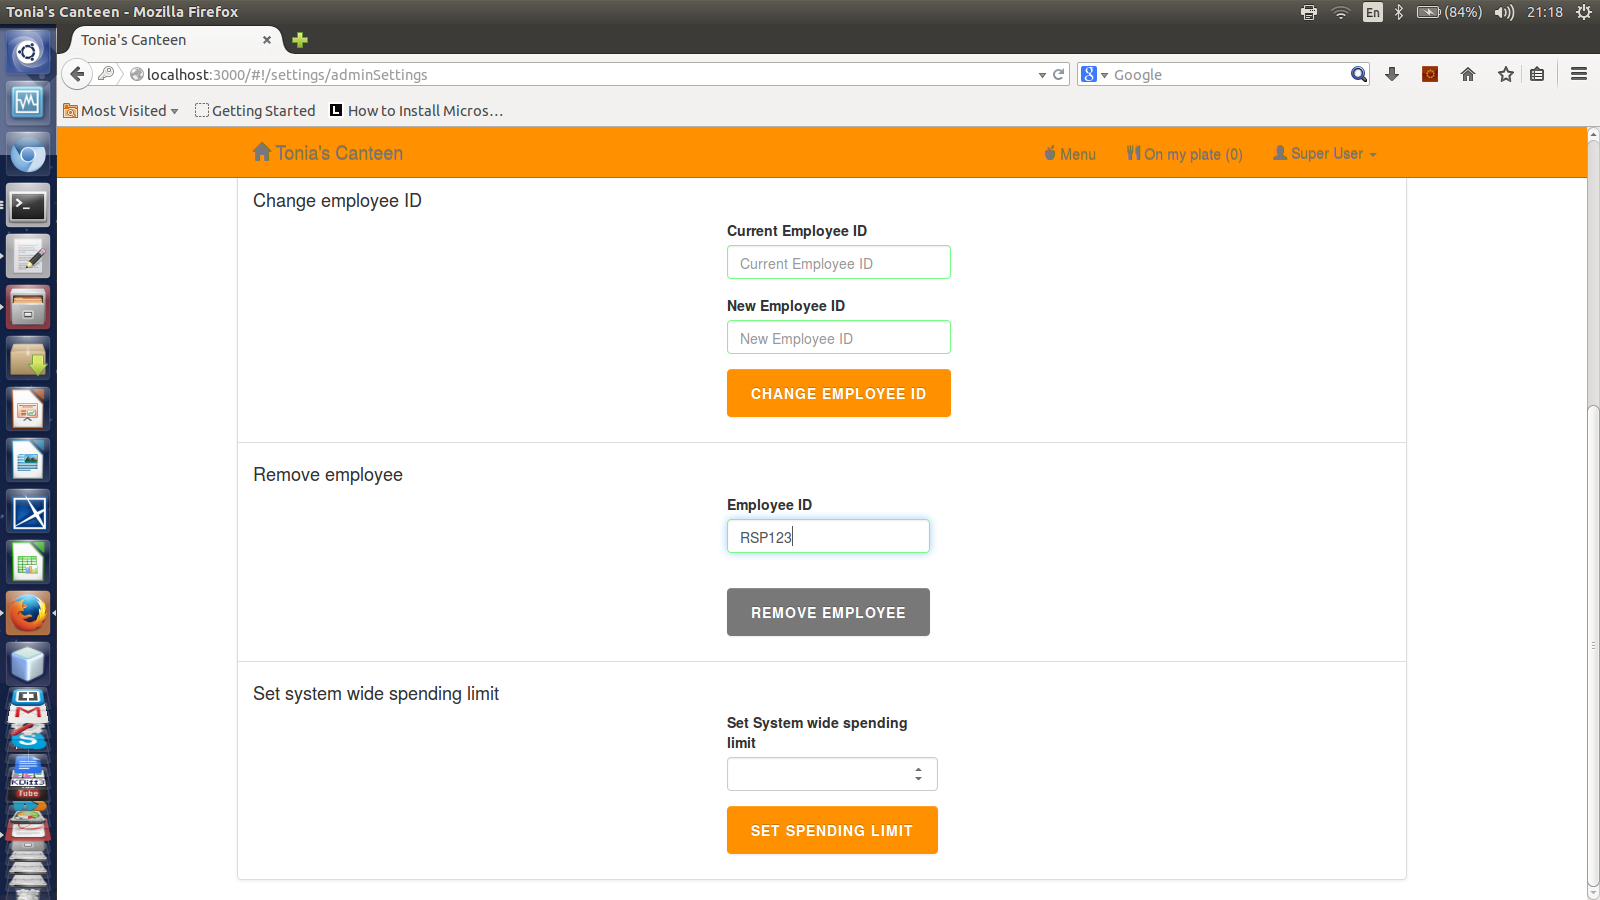
\includegraphics[width=1.0\textwidth]{screenshots/removeUser.png}
    \caption{The admin page - superuser can remove users from the system} 
\end{figure}

\begin{figure}[H]
  \centering
    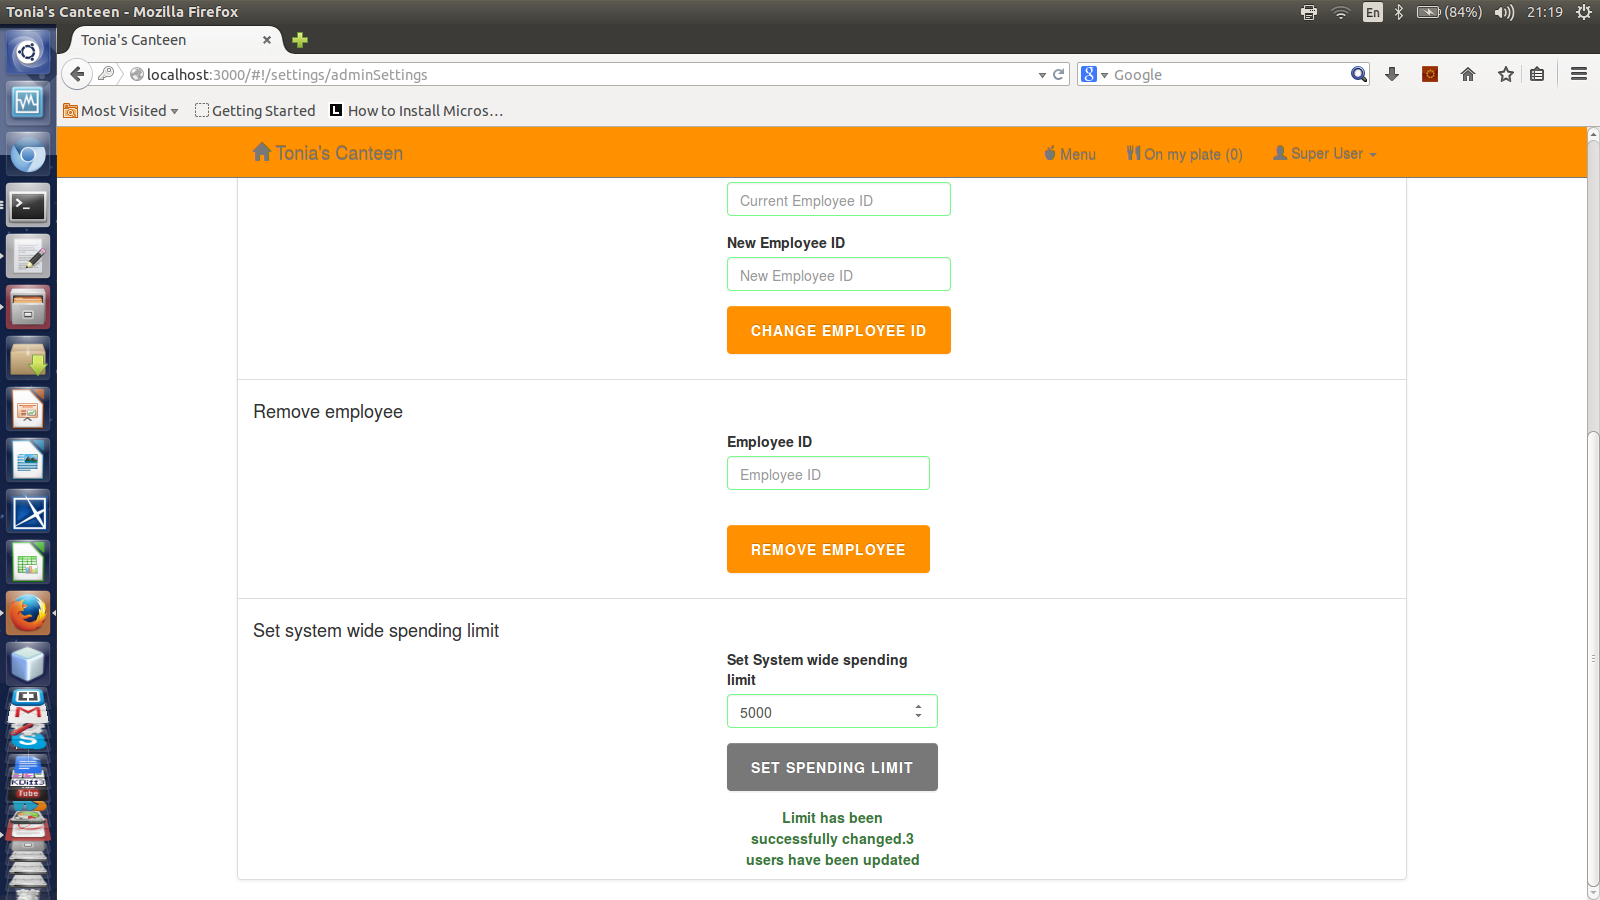
\includegraphics[width=1.0\textwidth]{screenshots/setLimit.png}
    \caption{The admin page - superuser can set the monthly spending limit for the users} 
\end{figure}
%%-----------------------superuser audits----------------------
\subsection{Superuser: The "Audits" Page} 
On this page, the superuser will be able to generate a thorough audit trail to trace all actions performed in the system for a specified period. There is a dropdown menu where the superuser can customize the search results to only view an audit for a particular type of action performed in the system.
\begin{figure}[H]
  \centering
    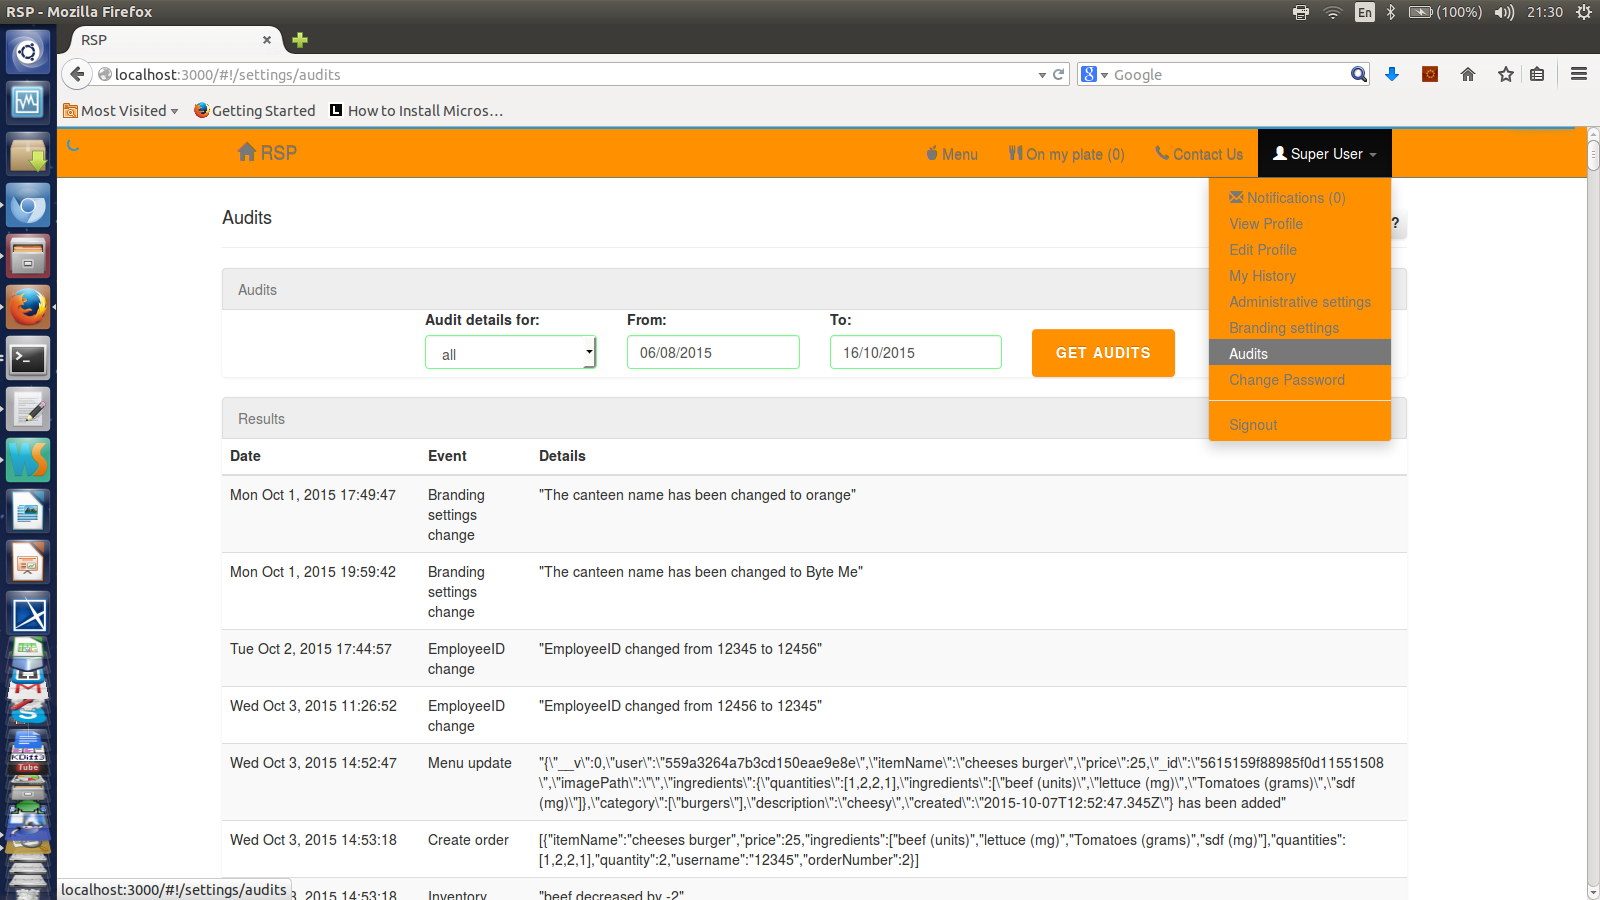
\includegraphics[width=1.0\textwidth]{screenshots/auditsAll.png}
    \caption{The audit page - superuser can view the audit trail for all actions performed in the system for a specified period. } 
\end{figure}

\begin{figure}[H]
  \centering
    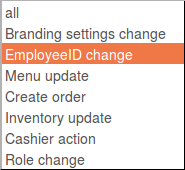
\includegraphics[width=1.0\textwidth]{screenshots/Menu_001.png}
    \caption{The audit page - the dropdown menu for the field to select audit details contains the following actions, more specifically all the main actions a user can perform in the system} 
\end{figure}

\begin{figure}[H]
  \centering
    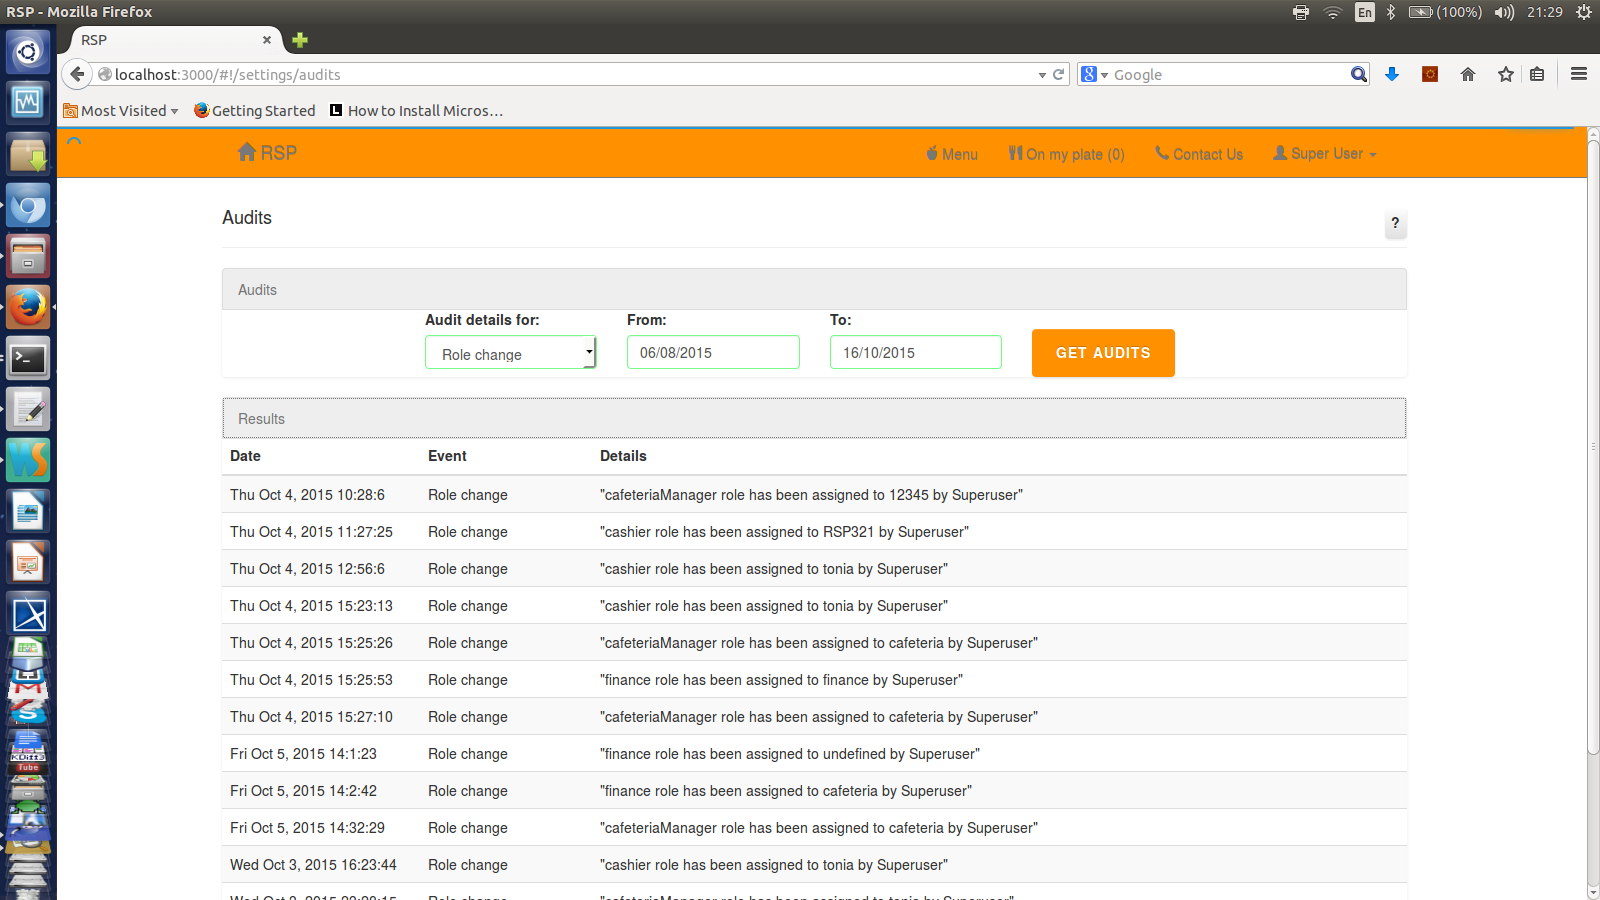
\includegraphics[width=1.0\textwidth]{screenshots/auditRole.png}
    \caption{The audit page - if the superuser selects one of the options, the audit trail is limited to that option} 
\end{figure}
%%-----------------------branding settings superuser----------------------
\subsection{Superuser: The "Branding Settings" Page} 
There are two sections on this page. One where the user can change the canteen name, by merely typing in a new name over the old name in the allocated textbox, and another where the superuser can add and remove carousel images for the cover image slides on the home page. The superuser can also configure the colour scheme for the system. The superuser can also add the contact details for the canteen that will be displayed on the contacts page
\begin{figure}[H]
  \centering
    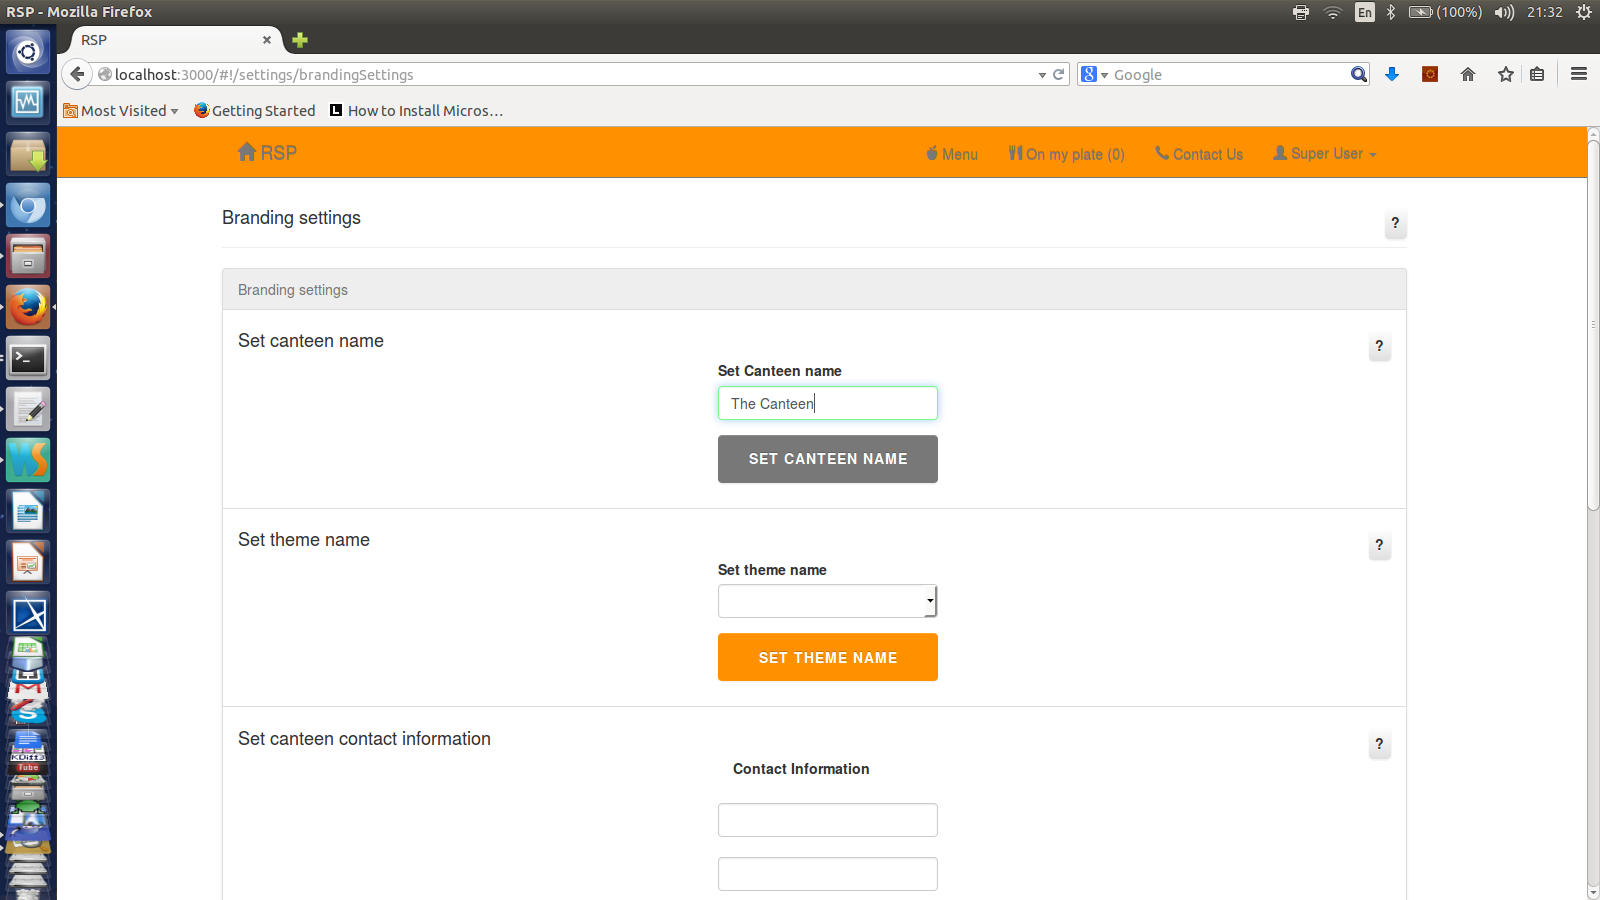
\includegraphics[width=1.0\textwidth]{screenshots/canteenName.png}
    \caption{The branding settings page - superuser can change the canteen name}
\end{figure}

\begin{figure}[H]
  \centering
    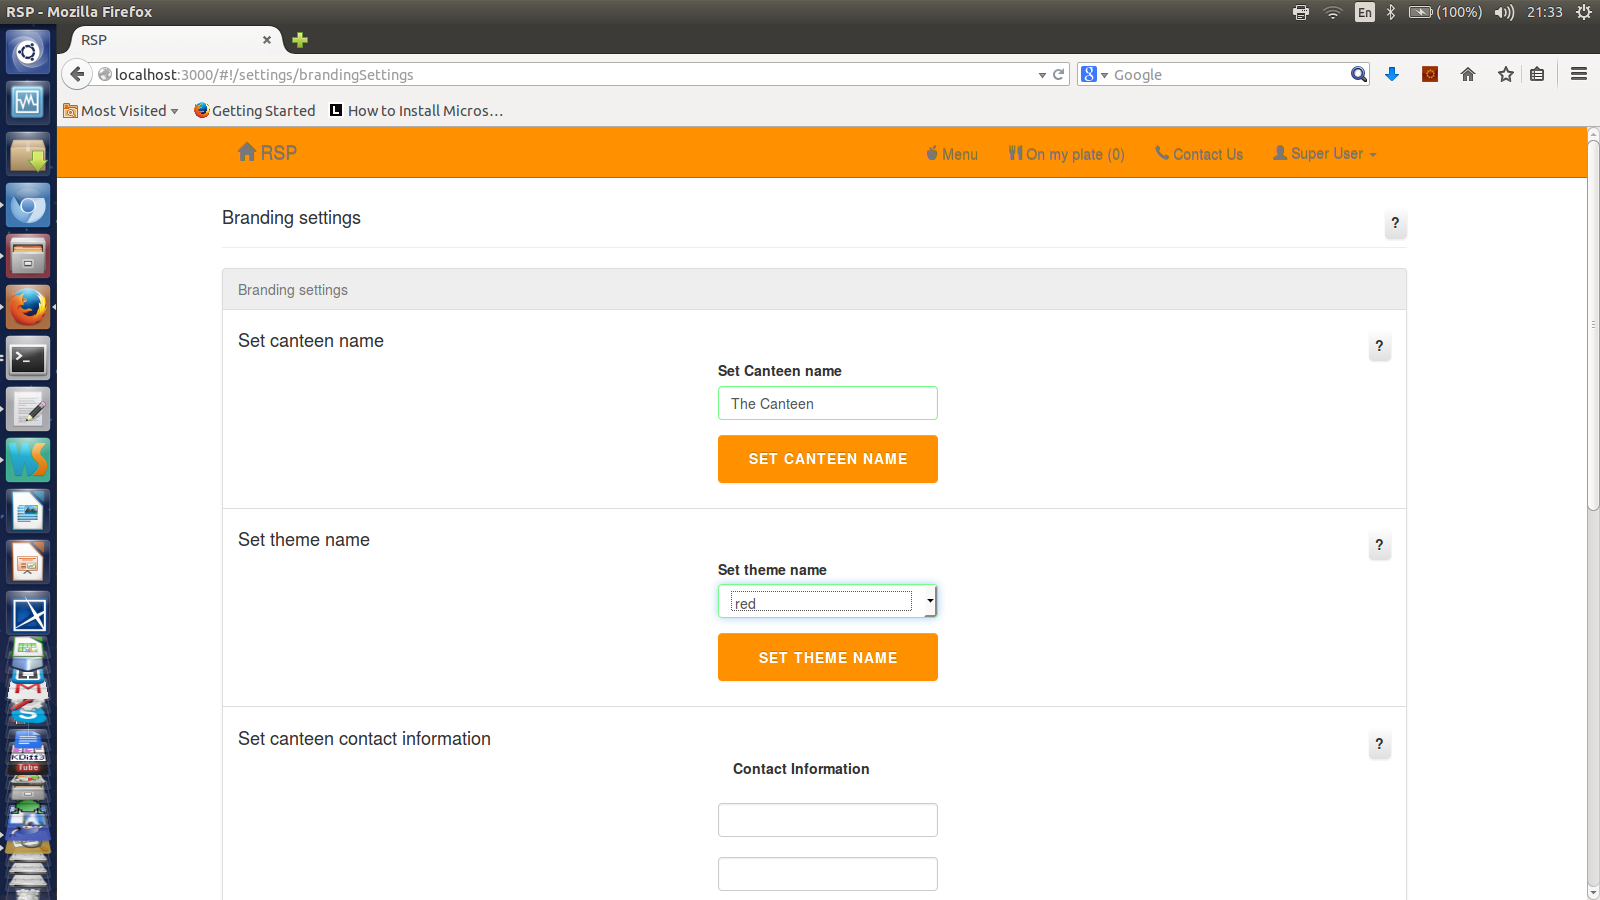
\includegraphics[width=1.0\textwidth]{screenshots/setTheme1.png}
    \caption{The branding settings page - superuser can change the canteen name}
\end{figure}

\begin{figure}[H]
  \centering
    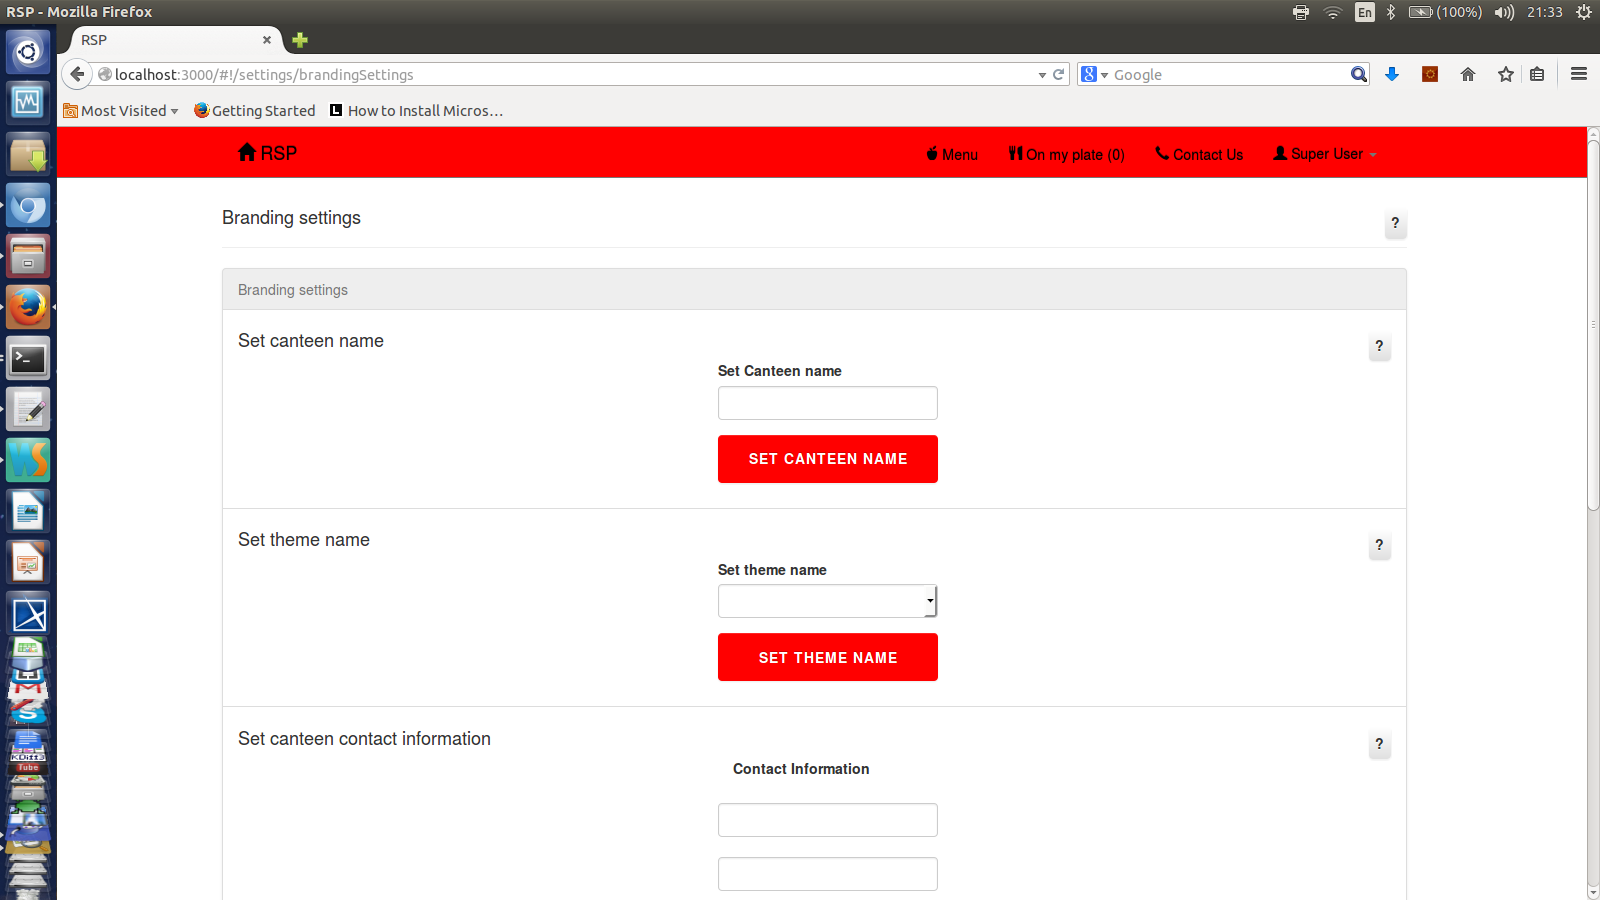
\includegraphics[width=1.0\textwidth]{screenshots/setTheme2.png}
    \caption{The branding settings page - the colour scheme of the system has now changed}
\end{figure}

\begin{figure}[H]
  \centering
    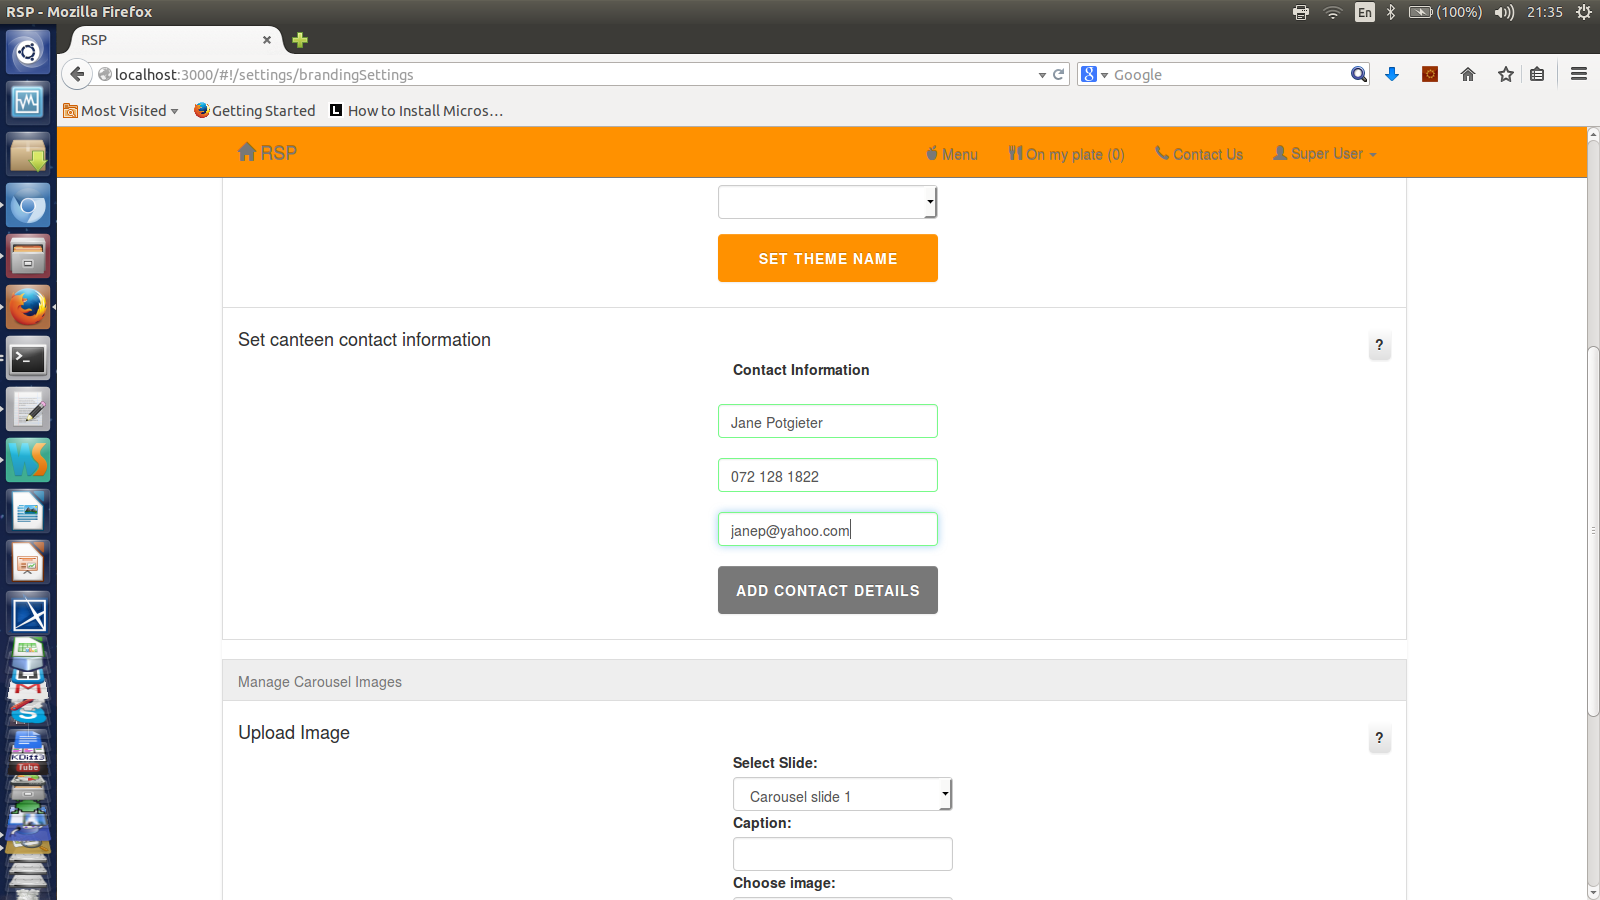
\includegraphics[width=1.0\textwidth]{screenshots/addContactInfo.png}
    \caption{The branding settings page - the contact information can be added in the appropriate boxes}
\end{figure}

\begin{figure}[H]
  \centering
    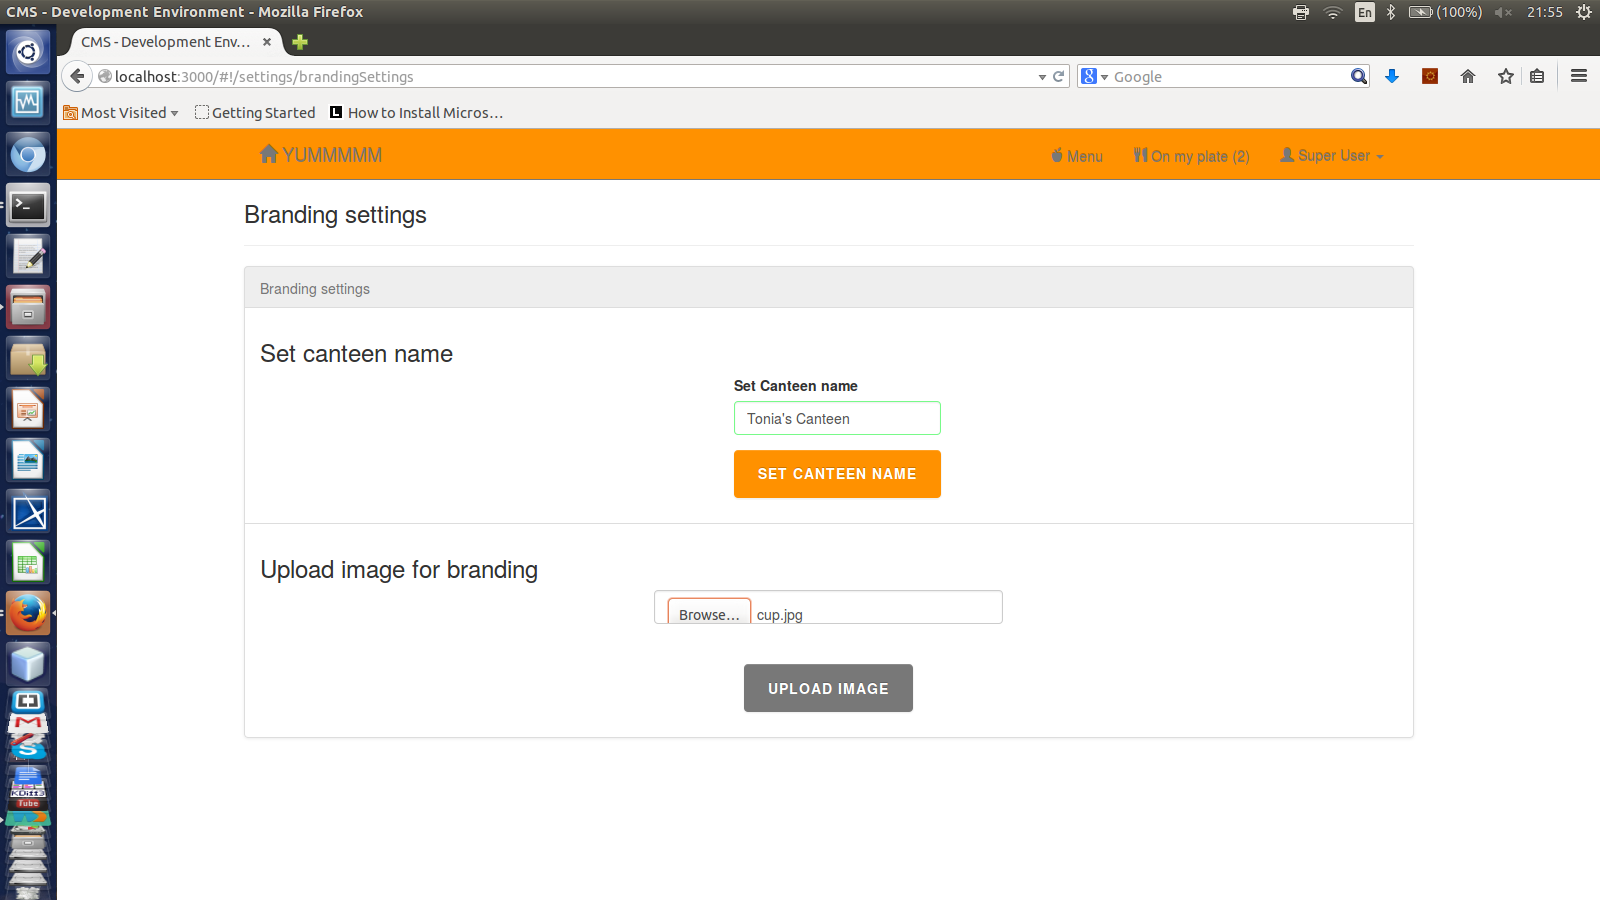
\includegraphics[width=1.0\textwidth]{screenshots/coverImage.png}
    \caption{The branding settings page - superuser can add/remove the images in the carousel} 
\end{figure}

\begin{figure}[H]
  \centering
    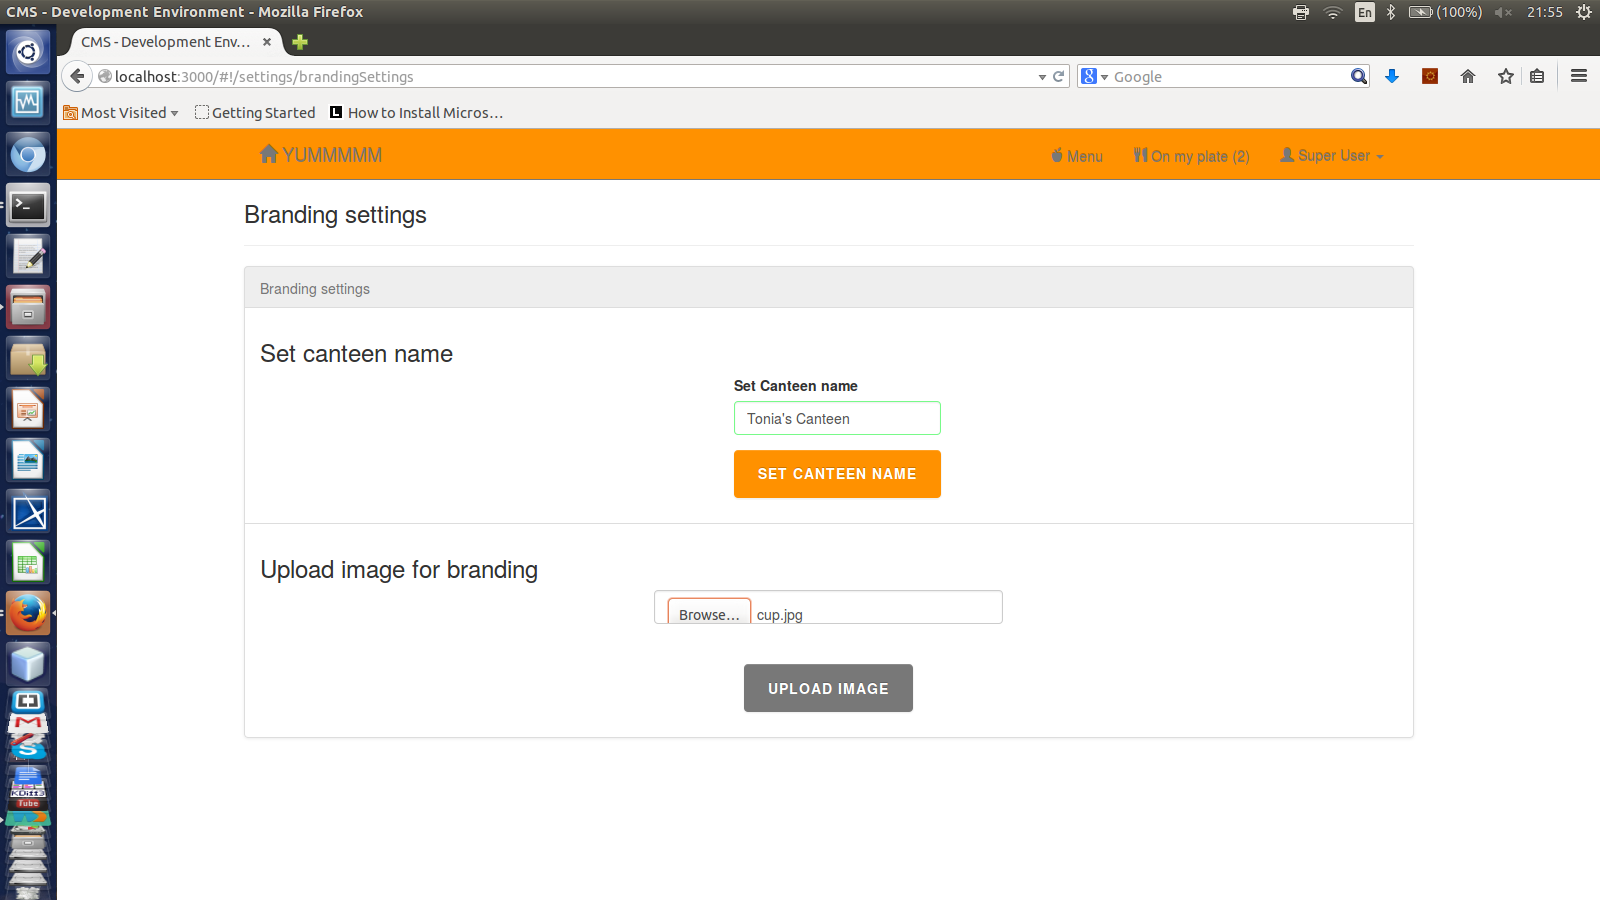
\includegraphics[width=1.0\textwidth]{screenshots/coverImage.png}
    \caption{The page will redirect to the carousel after an image has been added to a carousel slide and the new image will be displayed as follows} 
\end{figure}
%%-----------------------caf man - manage inventory----------------------

\subsection{Cafeteria Manager: The "Manage Inventory" Page}
This page is available to the cafeteria manager under the dropdown menu on the navigation pane. This is where the cafeteria manager adds inventory items to be used when an actual meal is stored in the menu in order to keep track of stock to note when a specific meal item is out of stock. These inventory items can be deleted, updated and searched for. 

\begin{figure}[H]
  \centering
    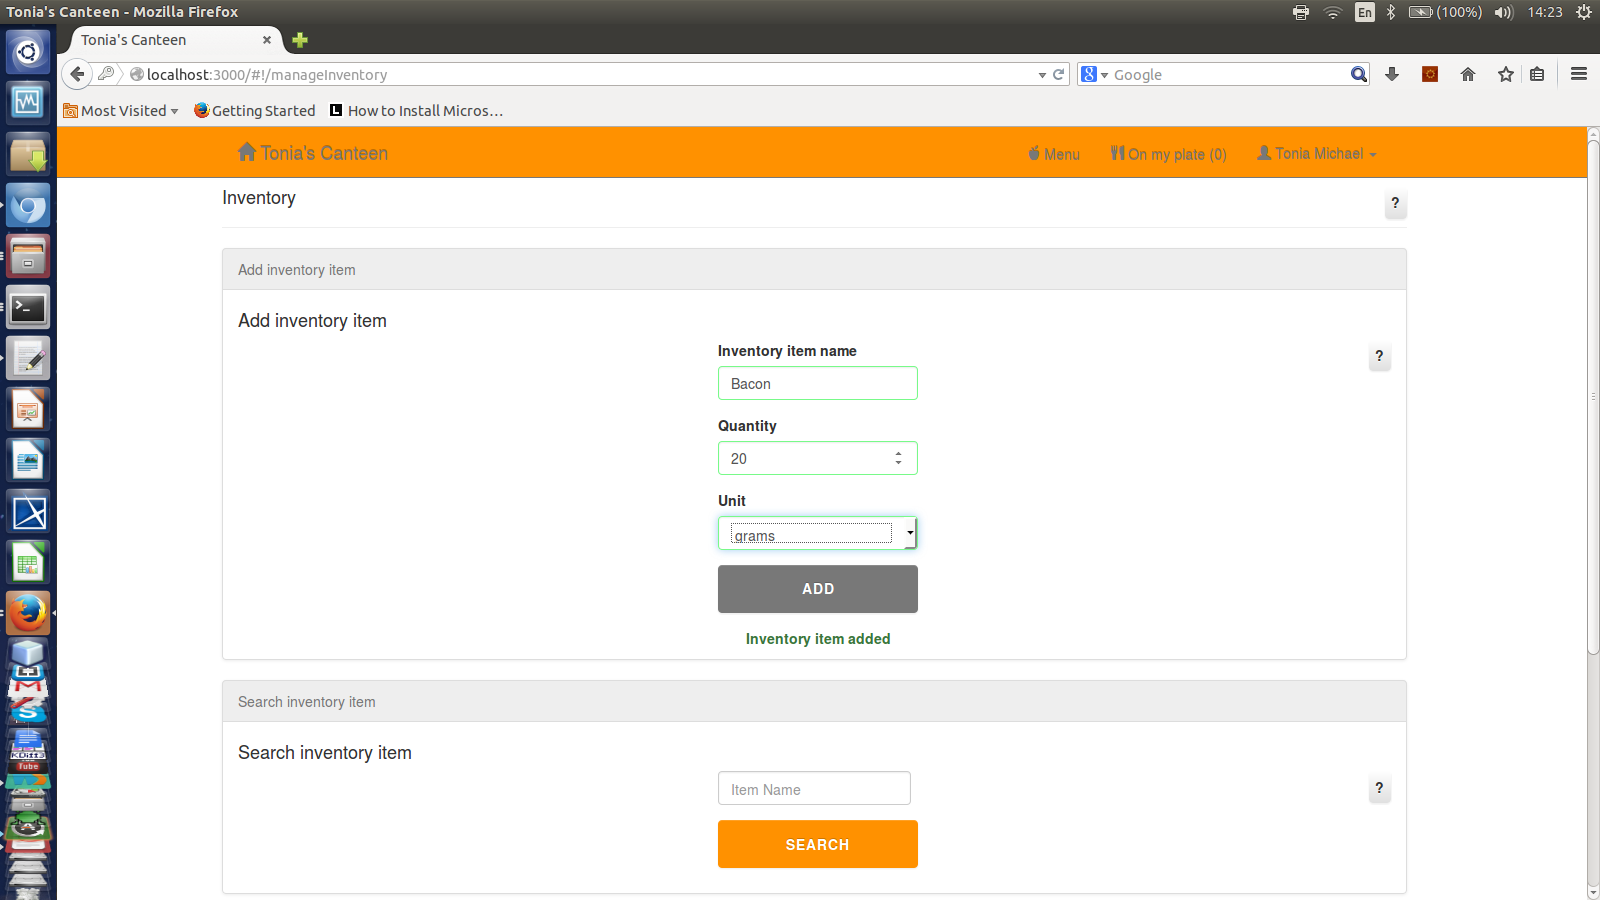
\includegraphics[width=1.0\textwidth]{screenshots/addInv.png}
    \caption{The manage inventory page - Cafeteria Manager can add inventory items}
\end{figure}

\begin{figure}[H]
  \centering
    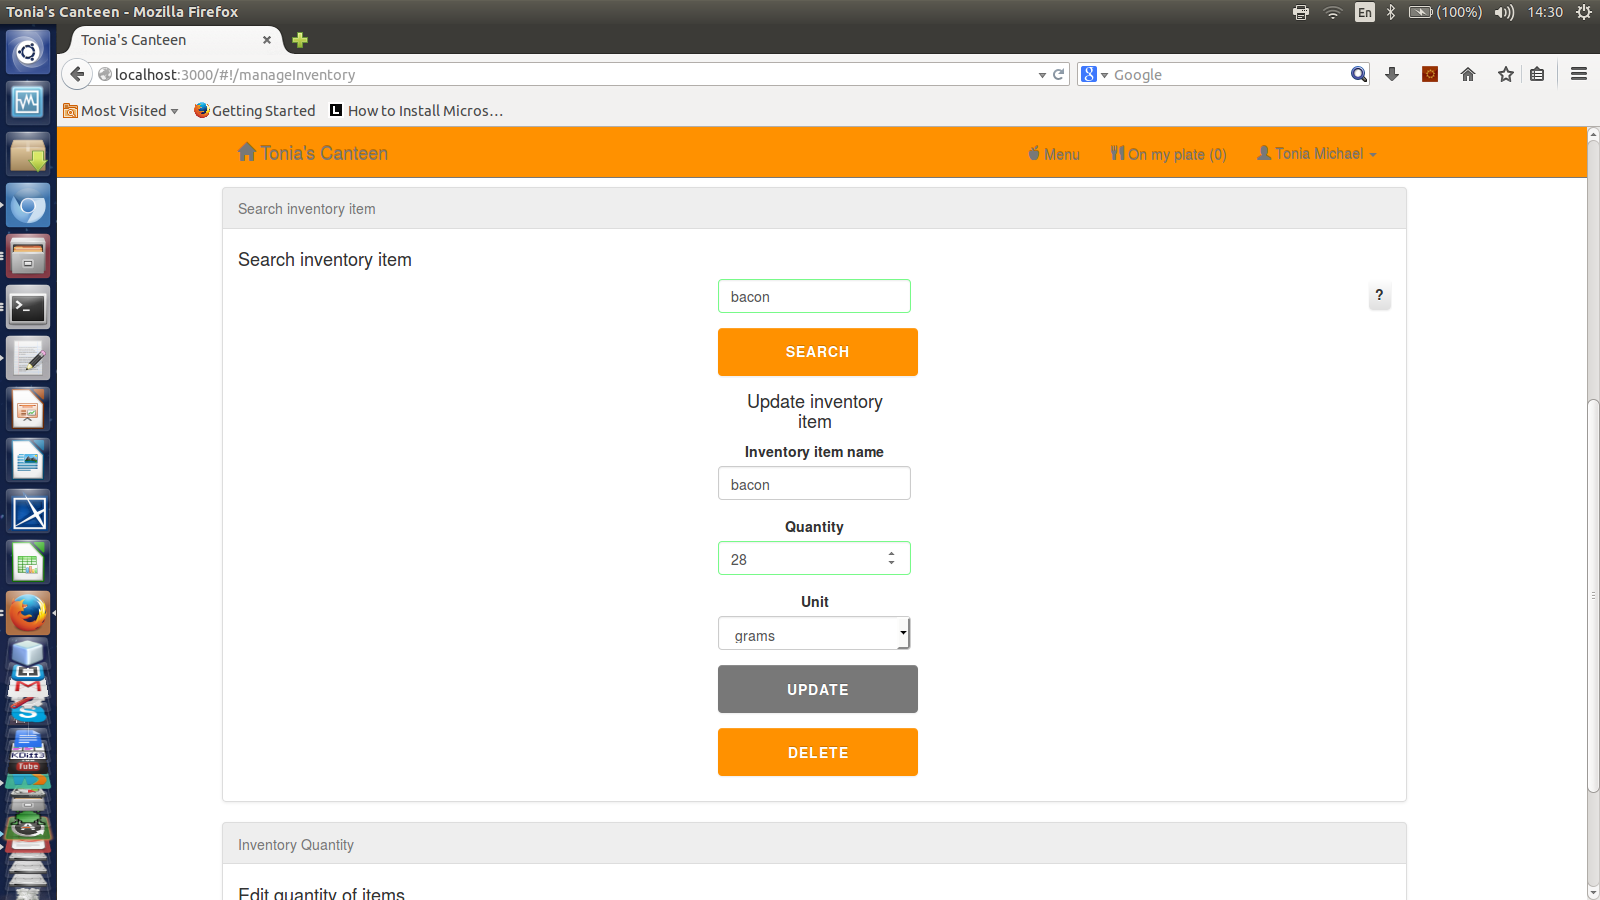
\includegraphics[width=1.0\textwidth]{screenshots/updateInv.png}
    \caption{The manage inventory page - Cafeteria Manager can update and delete inventory items}
\end{figure}
%%-----------------------Caf man manage menu----------------------
\subsection{Cafeteria Manager: The "Manage Menu" Page}
This is the page where the cafeteria manager adds menu items so that these can be displayed on the menu page found under the menu tab. The items can also be updated, deleted and searched for. The cafeteria manager can also add categories to the dynamic menu page. The cafeteria manager can also add images for each menu item to be displayed on the menu page.

\begin{figure}[H]
  \centering
    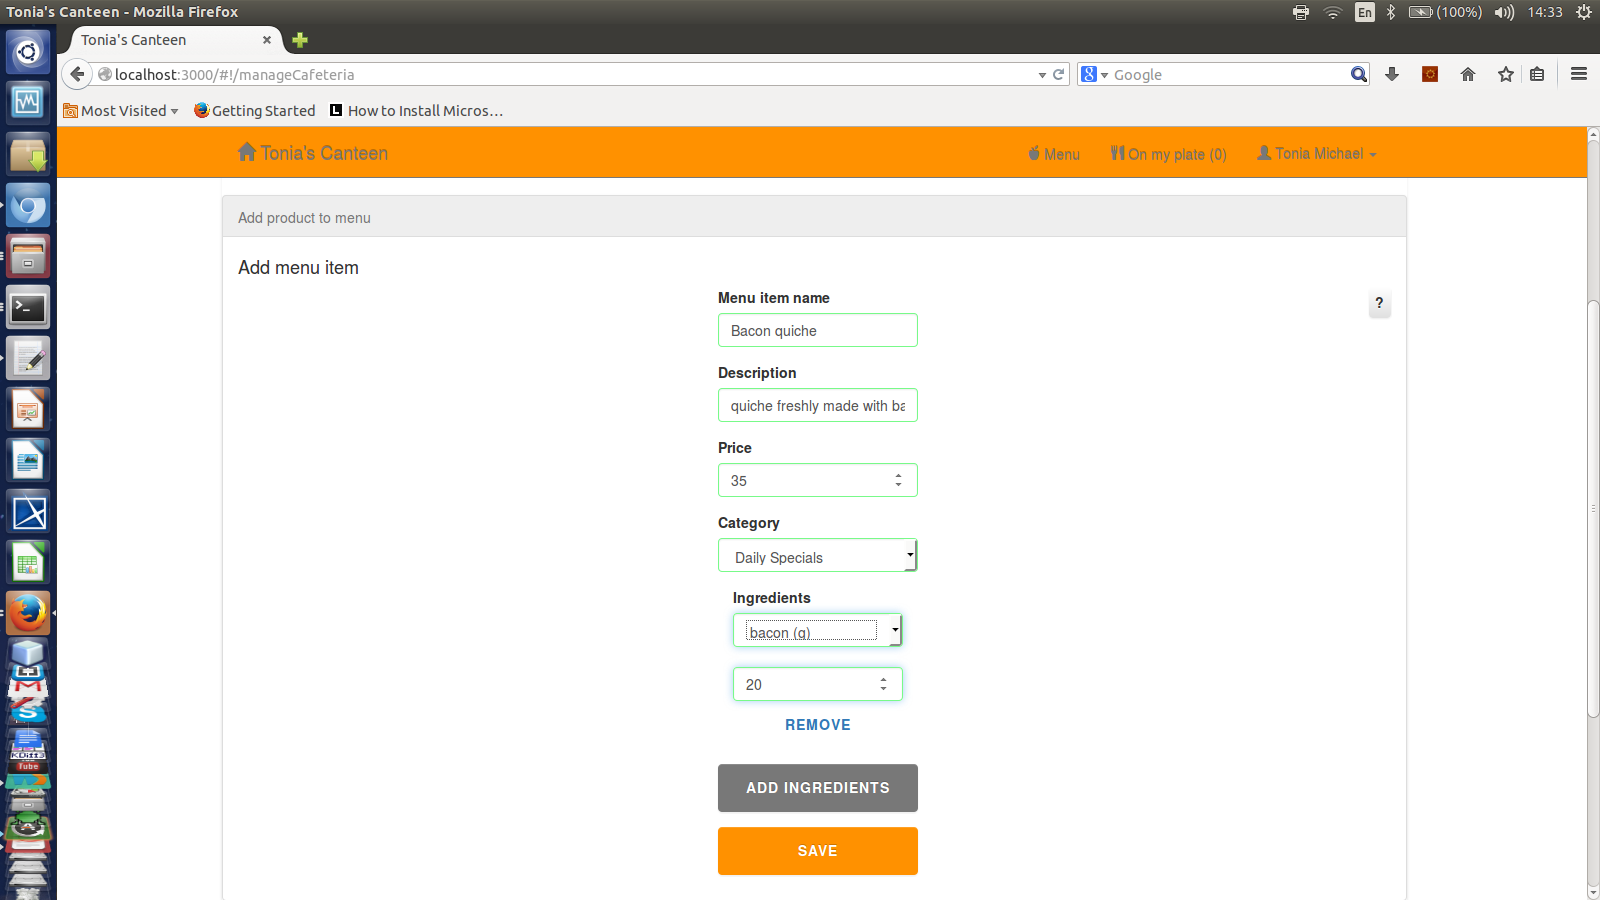
\includegraphics[width=1.0\textwidth]{screenshots/addMenu.png}
    \caption{The manage menu page - Cafeteria Manager can add menu items}
\end{figure}

\begin{figure}[H]
  \centering
    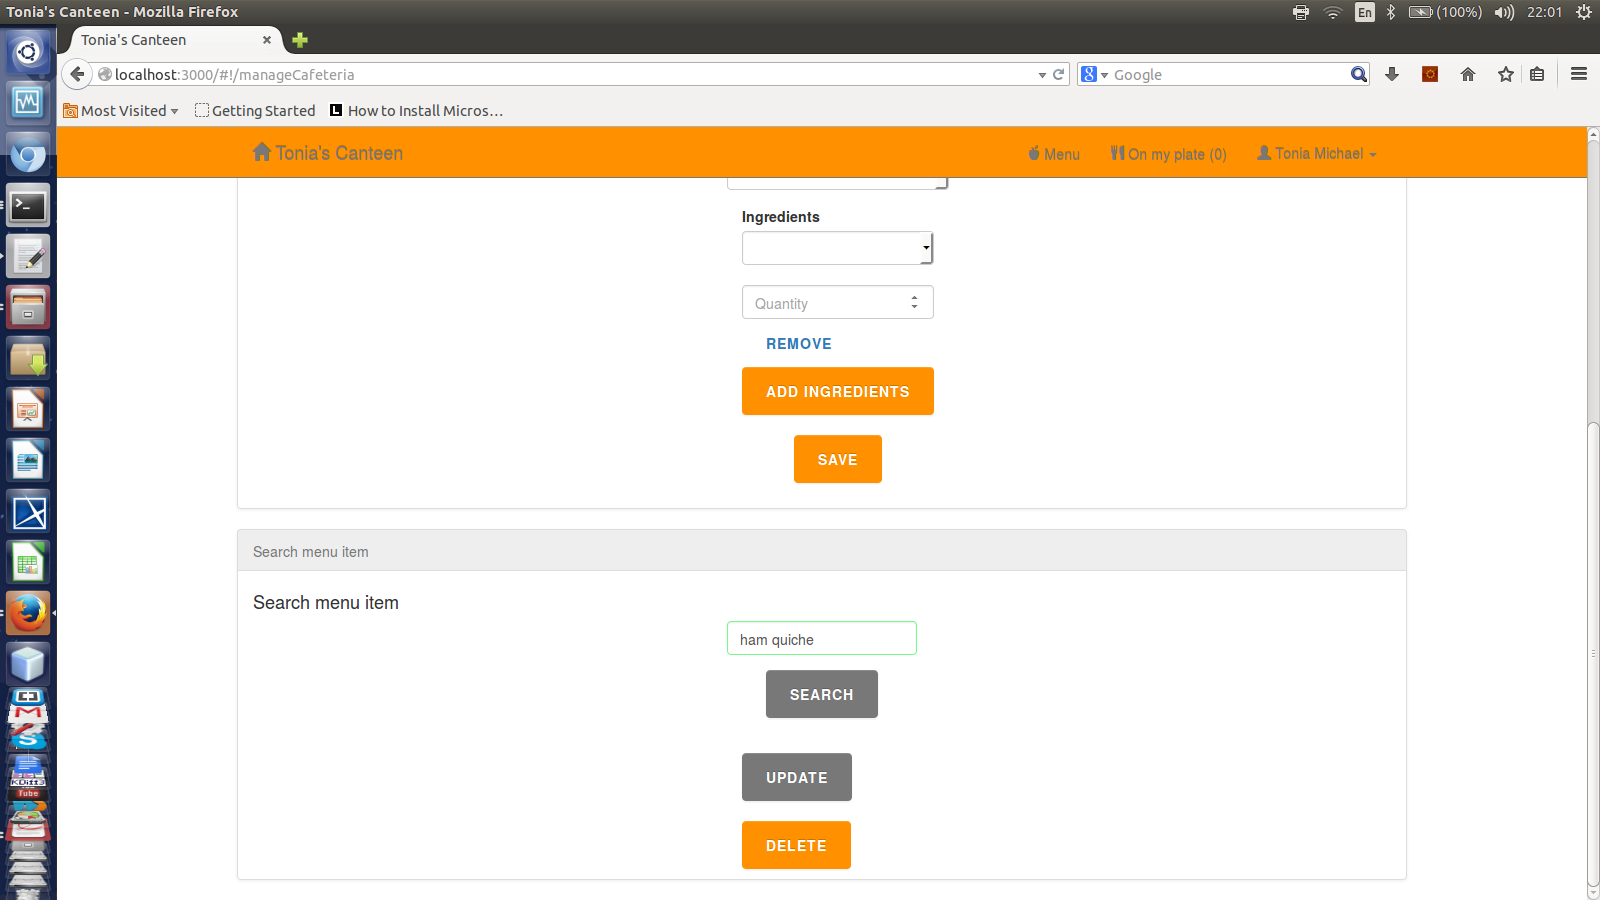
\includegraphics[width=1.0\textwidth]{screenshots/searchMenuItem.png}
    \caption{The manage menu page - Cafeteria Manager can search for menu items and proceed to update, delete or upload an image for the menu item to be displayed on the menu}
\end{figure}

\begin{figure}[H]
  \centering
    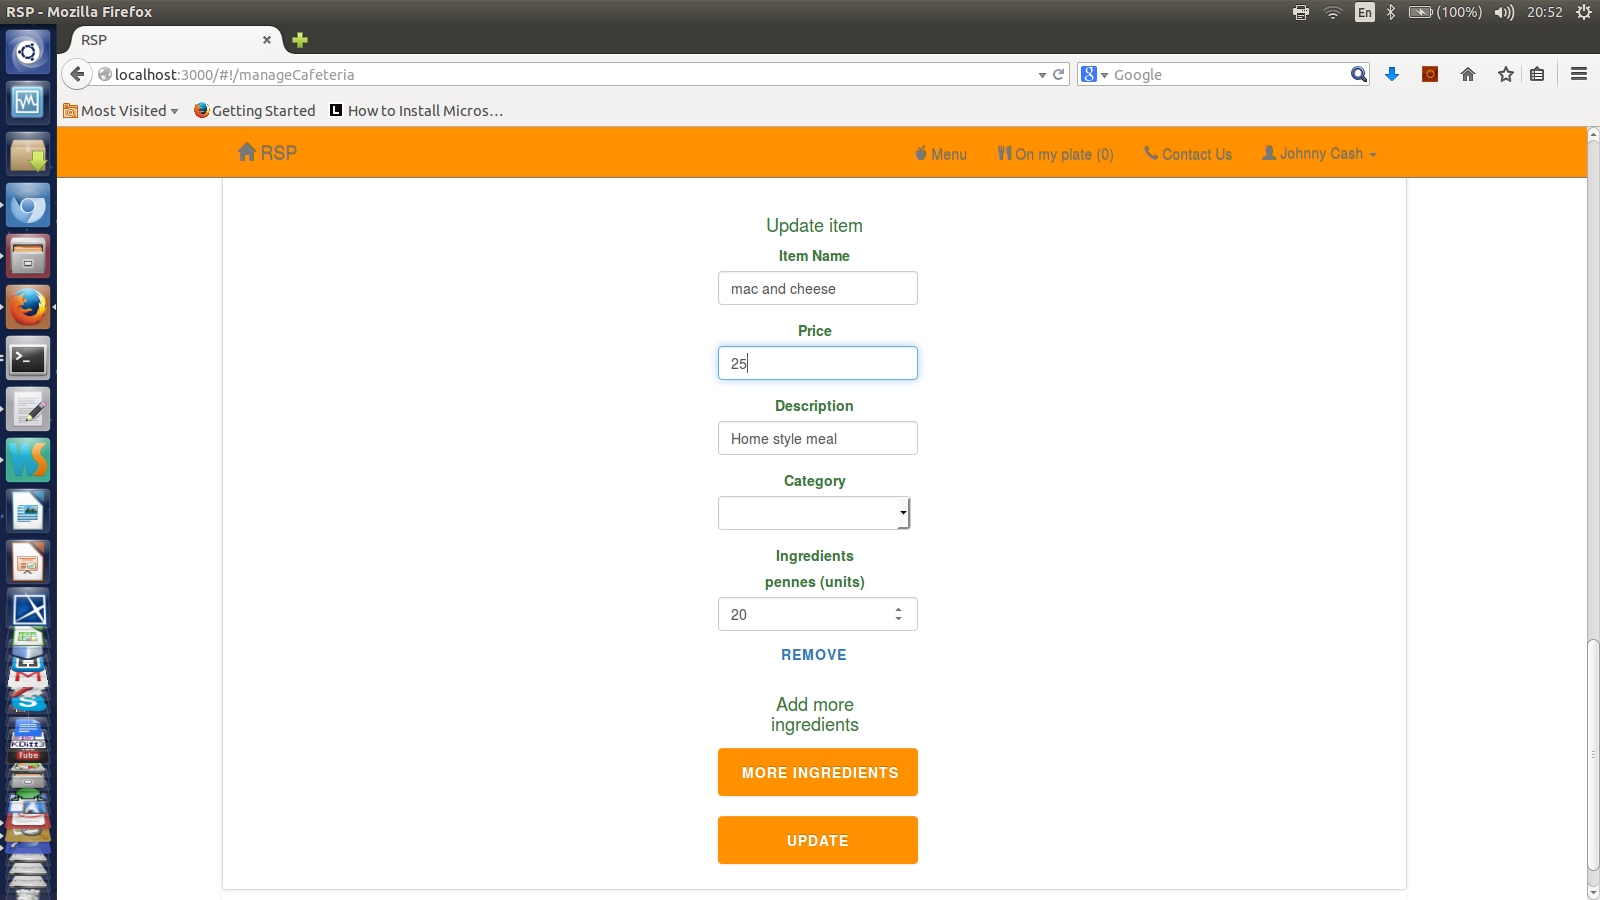
\includegraphics[width=1.0\textwidth]{screenshots/updateMenu.png}
    \caption{The manage menu page - Cafeteria Manager can update menu items}
\end{figure}

\begin{figure}[H]
  \centering
    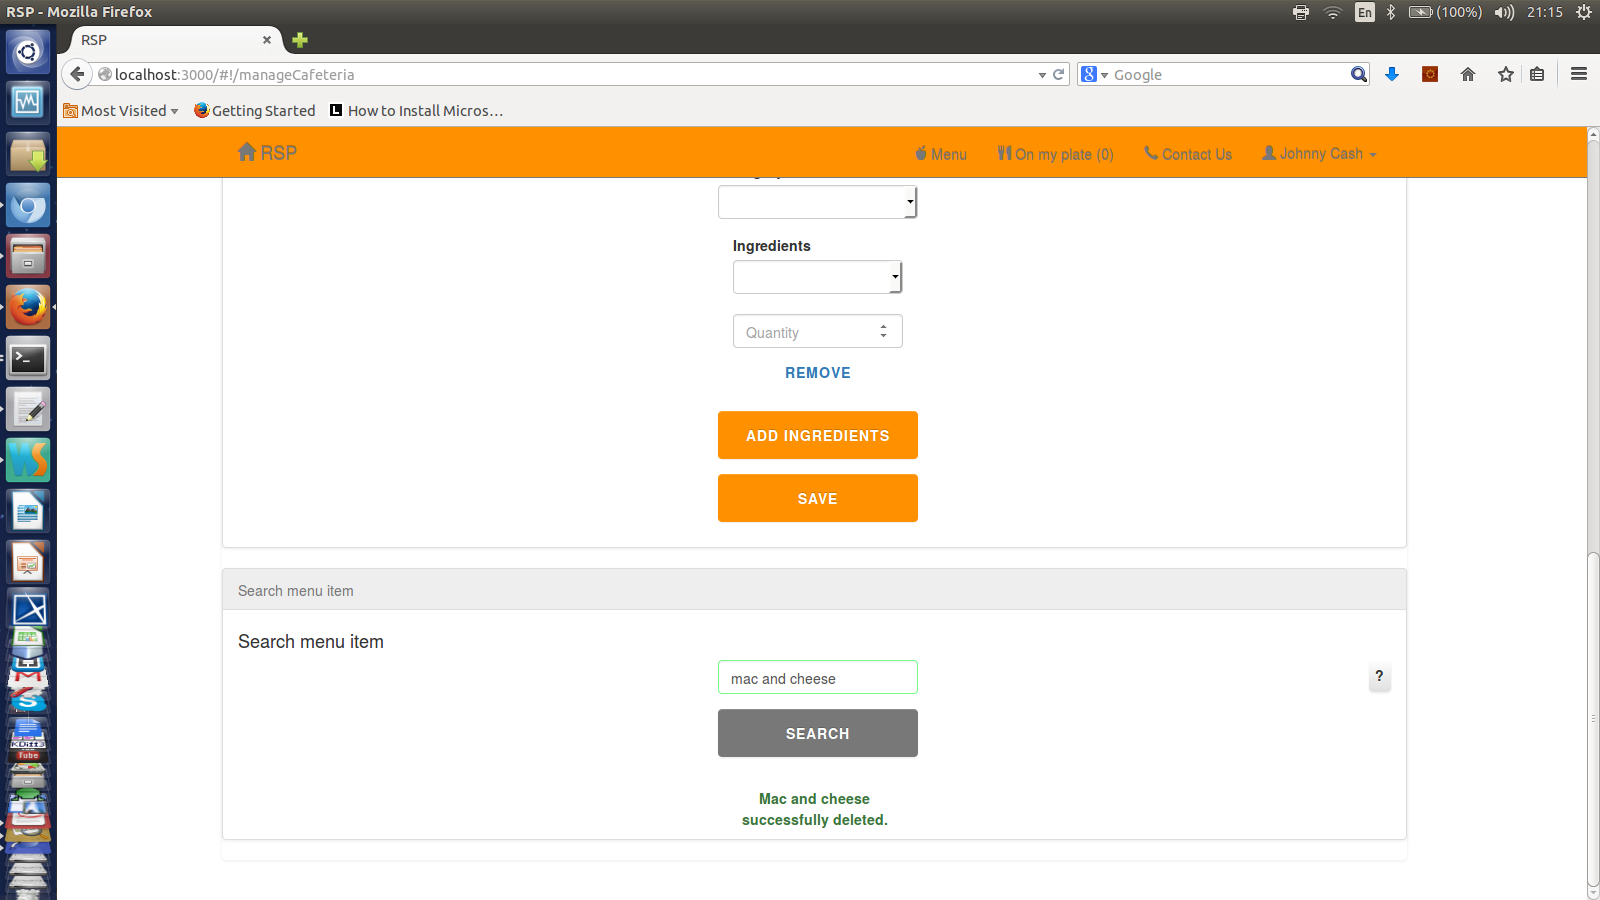
\includegraphics[width=1.0\textwidth]{screenshots/deleteMenu.png}
    \caption{The manage menu page - Cafeteria Manager can delete menu items}
\end{figure}

\begin{figure}[H]
  \centering
    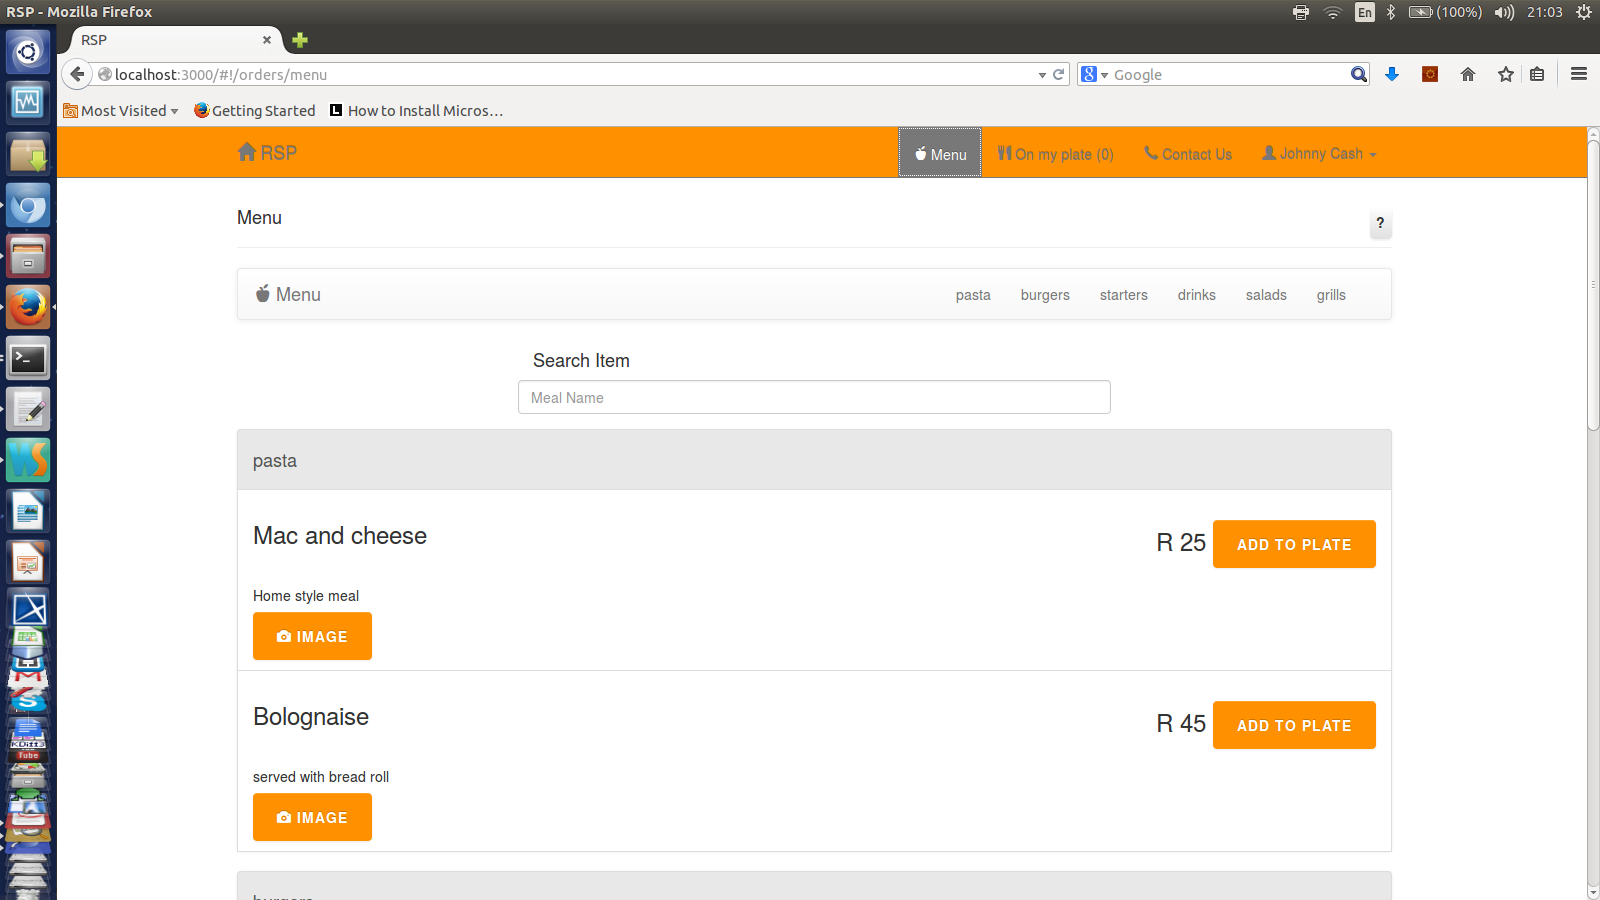
\includegraphics[width=1.0\textwidth]{screenshots/beforePasta.png}
    \caption{The menu page indicating a navigation bar of dynamically added categories. The cafeteria manager can proceed to add more categories as is shown in the successive screenshot }
\end{figure}
\begin{figure}[H]
  \centering
    \includegraphics[width=1.0\textwidth]{screenshots/addPasta.png}
    \caption{The manage menu page - Cafeteria Manager can add new menu categories}
\end{figure}
\begin{figure}[H]
  \centering
    \includegraphics[width=1.0\textwidth]{screenshots/afterPasta.png}
    \caption{The menu page - the added category is now displayed on the navigation pane}
\end{figure}
\subsection{Cafeteria Manager: The "Menu items statistics" Page}
The purpose of this page is to allow the cafeteria manager to keep tabs on which menu items are most popular and to keep track of which menu items are being purchased during specific periods of time. This is to alleviate the problem of the canteen frequently running out stock.

\begin{figure}[H]
  \centering
    \includegraphics[width=1.0\textwidth]{screenshots/menuStats1.png}
    \caption{The Menu Items Statistics page - the cafeteria manager can generate a graph to view menu items sold for a specific period of time}
\end{figure}

\begin{figure}[H]
  \centering
    \includegraphics[width=1.0\textwidth]{screenshots/menuStats2.png}
    \caption{The Menu Items Statistics page - the generated graph will be displayed as follows, grouping menu items by the menu categories}
\end{figure}

\begin{figure}[H]
  \centering
    \includegraphics[width=1.0\textwidth]{screenshots/menuStats25.png}
    \caption{The Menu Items Statistics page - the generated graph will be displayed as follows, grouping menu items by the menu categories}
\end{figure} 
 
\begin{figure}[H]
  \centering
    \includegraphics[width=1.0\textwidth]{screenshots/menuStats3.png}
    \caption{The Menu Items Statistics page - the cafeteria manager can generate a graph to view a specific number of the most popular menu items for a specific period of time}
\end{figure}

\begin{figure}[H]
  \centering
    \includegraphics[width=1.0\textwidth]{screenshots/menuStats4.png}
    \caption{The Menu Items Statistics page -the generated graph will be displayed as follows, grouping the most popular items by category}
\end{figure}

\begin{figure}[H]
  \centering
    \includegraphics[width=1.0\textwidth]{screenshots/menuStats4.png}
    \caption{The Menu Items Statistics page -the generated graph will be displayed as follows, displaying the most popular items in descending order}
\end{figure}

\subsection{Cafeteria Manager: The "Inventory statistics" Page}
The purpose of this page is to allow the cafeteria manager to keep track of which inventory items are being purchased during specific periods of time. This is to alleviate the problem of the canteen frequently running out stock.

\begin{figure}[H]
  \centering
    \includegraphics[width=1.0\textwidth]{screenshots/invStats1.png}
    \caption{The Inventory Statistics page - the cafeteria manager can generate a graph to view the inventory items used for a specific period of time }
\end{figure}

\subsection{Cashier: The "Process Orders" Page}
This page is for use by the cashier. Orders that are "open" will be displayed on the page. Orders can be marked as ready, paid or collected. When the order is marked as ready, the button will disappear and the employee will be sent an email informing them to come collect their order. When the "Employee Paid" button is clicked, the cashier will choose whether it was a cash or credit purchase and the amount will be deducted accordingly from the user's account.

\begin{figure}[H]
  \centering
    \includegraphics[width=1.0\textwidth]{screenshots/cashier.png}
    \caption{The process orders page - The cashier is authorized to facilitate these transactions}
\end{figure}
 %make a graphic for ready button disappearing

\begin{figure}[H]
  \centering
    \includegraphics[width=1.0\textwidth]{screenshots/cashierCredit.png}
    \caption{The process orders page - The cashier can select the appropriate radio button as to whether the employee is paying with cash or credit.}
\end{figure}

\begin{figure}[H]
  \centering
    \includegraphics[width=1.0\textwidth]{screenshots/noPaymentMethSelected.png}
    \caption{The process orders page - If the cashier does not select a payment method, an error message will be alerted}
\end{figure}

\begin{figure}[H]
  \centering
    \includegraphics[width=1.0\textwidth]{screenshots/empPaid.png}
    \caption{The process orders page - The order will be removed from the page when the cashier clicks the "Employee paid" button. Order 7 - The cheese salad is now removed from the page due to this}
\end{figure}

\subsection{Financial Manager: The "View Employee Bills" Page}
There is a field labelled "Employee Id" and it is in here where a user will type in the employee ID of the employee whose bill the finance manager would like to view. The date ranges can also be selected here.

\begin{figure}[H]
  \centering
    \includegraphics[width=1.0\textwidth]{screenshots/bill1.png}
    \caption{The View Employee Bills Page - The employee ID of the employee whose bill would like to be viewed is entered in the box as shown.}
\end{figure}

\begin{figure}[H]
  \centering
    \includegraphics[width=1.0\textwidth]{screenshots/bill2.png}
    \caption{The View Employee Bills Page - The date ranges can be specified by using the drop down calender}
\end{figure}

\begin{figure}[H]
  \centering
    \includegraphics[width=1.0\textwidth]{screenshots/bill3.png}
    \caption{The View Employee Bills Page - Once the "Display Bill" button is clicked, the pdf will be dowloaded and the invoice will look as shown.}
\end{figure}


\section{Troubleshooting}
\subsection{Problems with setting up the system}
If the system does not start up when you run the 'grunt' command, either of the following procedures can be followed:
\begin{itemize}
\item Ensure you have an active internet connection as the system requires an internet connection.
\item Ensure you have MongoDB running in a separate terminal. \\
	The line \begin{verbatim}
		Waiting for connections on port 27017
	\end{verbatim} should be displayed at the end of the Mongo terminal.
\item If the above does not solve the problem, the command npm update should be run from inside the CMS directory:
	\begin{verbatim}
		~/Cafeteria Management System$ npm update
	\end{verbatim}
\item If the problem persists the following commands should be run in order:
	\begin{verbatim}
		~/Cafeteria Management System$ bower install
	\end{verbatim} 
	\begin{verbatim}
		~/Cafeteria Management System$ npm install
	\end{verbatim} 
	\begin{verbatim}
		~/Cafeteria Management System$ npm update
	\end{verbatim}
\end{itemize}
\end{document}
